\input{/Users/daniel/github/config/preamble-por.sty}%available at github.com/danimalabares/config %\input{/Users/daniel/github/config/thms-por.sty}%available at github.com/danimalabares/config
\usepackage{mdframed}

\newcommand{\rightlooparrow}{\mathbin{
    \vbox{\openup-10.25pt\halign{\hss$##$\hss\cr\circ\cr\longrightarrow\cr}}
}}

\begin{document}
\bibliographystyle{alpha}
\begin{minipage}{\textwidth}
	\begin{minipage}{1\textwidth}
		\hfill Daniel González Casanova Azuela
		
		{\small Prof. Luis Florit\hfill\href{https://github.com/danimalabares/rg}{github.com/danimalabares/rg}}
	\end{minipage}
\end{minipage}\vspace{.2cm}\hrule

\vspace{10pt}
{\huge Exercícios de Geometria Riemanniana}
\tableofcontents

\section{Exercícios do do Carmo}

\subsection{Capítulo 0}
\begin{thing4}{Exercise 2}\label{exer:2}\leavevmode
Prove que o fibrado tangente de uma variedade diferenciável \(M\) é orientável (mesmo que \(M\) não seja).
\end{thing4}

\begin{proof}[Solution]\leavevmode
Es porque la diferencial de los cambios de coordenadas está dada por la identidad y una matriz lineal. Sí, porque por definición las trivializaciones locales de \(TM\) preservan la primera coordenada \textbf{y} son isomorfismos lineales en la parte del espacio vectorial. Entonces queda que 
\[d(\varphi_U \circ \varphi_V^{-1})=\left(\begin{array}{@{}c|c@{}}
\operatorname{Id}&0\\
\hline
0&\xi \in \mathsf{GL}(n)\end{array}\right)\]
pero no estoy seguro de por qué \(\xi\) preservaría orientación, i.e. que tenga determinante positivo… a menos de que… 
\end{proof}

\begin{thing4}{Exercise 5}[Mergulho de \(P^2(\mathbb{R})\) em \(\mathbb{R}^4\) ]\label{exer:5}\leavevmode
Seja \(F:\mathbb{R}^3 \to \mathbb{R}^4\) dada por
\[F(x,y,z)=(x^2-y^2,xy,xz,yz),\qquad (x,y,z) = p \in \mathbb{R}^3.\]
Seja \(S^2 \subset \mathbb{R}^3\) a esfera unitária com centro na origem \(0 \in \mathbb{R}^3\). Oberve que a restrição \( \varphi:= F|_{S^2}\) é tal que \(\varphi(p)=\varphi(-p)\), e considere a aplicação \(\tilde{\varphi}:\mathbb{R}P^2 \to \mathbb{R}^4\) dada por
\[\tilde{ \varphi}([p])=\varphi(p),\qquad [p]\text{=clase de equivalência de \(p=\{p,-p\}\)} \]

Prove que
\begin{enumerate}[label=(\alph*)]
\item \(\tilde{\varphi}\) é uma imersão.
\item \(\tilde{\varphi}\) é biunívoca; junto com (a) e a compacidade de  \(\mathbb{R}P^2\), isto implica que \(\tilde{ \varphi}\) é um mergulho.
\end{enumerate}
\end{thing4}

\begin{proof}[Solution]\leavevmode
\begin{enumerate}[label=(\alph*)]
\item Considere a carta \(\{z=1\}\). A representação coordenada de \(\tilde{\varphi}\) vira
	\[(x,y) \longmapsto (x^2-y^2,xy,x,y)\]
cuja derivada como mapa \(\mathbb{R}^2 \to \mathbb{R}^4\) é
\[\begin{pmatrix} 2x& -2y\\y&x\\1&0\\0&1 \end{pmatrix} \]
que é injetiva. Agora pegue a carta \(\{x=1\}\). Então a representão coordenada de \(\tilde{ \varphi}\) vira
\[(y,z) \longmapsto (1-y^2,y,z,yz)\]
e tem derivada
\[\begin{pmatrix} -2y&0\\1&0\\0&1\\z&y \end{pmatrix} \]
que também é injetiva. Seguramente algo análogo acontece na carta \(\{y=1\}\).

\item \(\tilde{\varphi}\) é injetiva. Pegue dois pontos \(p_1:=[x_1:y_1:z_1]\) e \(p_2:=[x_2:y_2:z_2]\) e suponha que \(\tilde{\varphi}(p_1)=\tilde{\varphi}(p_2)\). I.e.,
	\[x_1^2-y_1^2=x_2^2-y_2^2,\qquad x_1y_1=x_2y_2,\qquad x_1z_1=x_2z_2, \qquad y_1z_1=y_2z_2\]
	Suponha primeiro que \(z_1 \neq  0\). Segue que
	\[x_1=\frac{z_2}{z_1}x_2, \qquad y_1=\frac{z_2}{z_1}y_2\]
	logo
	\[x_2^2-y_2^2=x_1^2-y_1^2=\left(\frac{z_2}{z_1}\right)^2(x_2^2-y_2^2)\implies z_2=z_1\implies x_1=x_2,\qquad y_1=y_2\]
	

	Em fim, uma imersão injetiva com domínio compacto é um mergulho porque é fechada: pegue um fechado no domínio, vira compacto, imagem é compacta, que é fechado. Pronto.
.
\end{enumerate}
\end{proof}

\begin{thing4}{Exercício 8}\label{exer:8}\leavevmode
\(\varphi:M_1\to M_2\) difeo local. Se \(M_2\) é orientável, então \(M_1\) é orientável.
\end{thing4}
\begin{proof}[Solução]\leavevmode
Defina: uma base \(\beta \subset T_pM\) é orientada se \(\varphi_*\beta\) é orientada em \(T_{\varphi(p)}M\). Tá bem definida porque \(\varphi\) é um difeomorfismo em \(p\), i.e. \(\varphi_*\) é isomorfismo. Para mostrar que é contínua à la Lee, qualquer vizinhança de um ponto \(p \in M_1\), a correspondente carta coordenada em \(\varphi(p)\), um marco coordenado nela e puxe (pushforward baix \(\varphi^{-1}\)) de volta para \(U\). Difeomorfismo e muito bom: o pushforward the campos vetoriais está bem definido. E por construção está orientado.
\end{proof}
\subsection{Capítulo 1}

\begin{thing4}{Exercise 1}\label{exer:1}\leavevmode
Prove que a aplicação antípoda \(A:S^n \to S^n\) dada por \(A(p)=-p\) é uma isometria de \(S^n\). Use este fato para introduzir uma métrica Riemanniana no espaço projetivo real \(\mathbb{R}P^{n}\) tal que a projeção natural \(\pi: S^n \to \mathbb{R}P^{n}\) seja uma isometria local.
\end{thing4}
\begin{proof}[Solution]\leavevmode
	Lembre que a métrica de \(S^n\) é a induzida pela métrica euclidiana, onde pensamos que \(T_pS^n \hookrightarrow T_p\mathbb{R}^{n+1}\). É claro que \(A\) é uma isometría de \(\mathbb{R}^n\), pois ela é a sua derivada (pois ela é linear), de forma que \(\left<v,w\right>_p=\left<-v,-w\right>_{A(p)}=\left<v,w\right>_{-p}\).

	É um fato geral que se as transformações de coberta preservam a métrica, obtemos uma métrica no quociente de maneira natural, i.e. para dois vetores \(v,w\in T_p\mathbb{R}P^n\) definimos \(\left<v,w\right>_p^{\mathbb{R}P^n}:=\left<\tilde{v},\tilde{w}\right>_{\tilde{p} \in \pi^{-1}(p)}\).

Para ver que a projeção natural é uma isometria local basta ver que a diferencial de \(A\) é um isomorfismo em cada ponto. Mas como ela é \(-A\), isso é claro.
\end{proof}

\begin{thing4}{Exercício 7}\label{exer:7}\leavevmode
Seja \(G\) um grupo de Lie compacto e conexo (\(\dim(G)=n\)). O objetivo do exercício é provar que \(G\) possui uma métrica bi-invariante. Para isto, prove as seguintes etapas:
\begin{enumerate}[label=(\alph*)]
\item Seja \(\omega\) uma \(n\)-forma diferencial em \(G\) invariante à esquerda, isto é, \(L_x^*\omega=\omega\), para todo  \(x\in G\). Prove que \(\omega\) é invariante à direita.

	\textit{Sugestão}: Para cada \(a \in Ga\), \(R_a ^*\omega\) é invariante à esqueda. Decorre daí que \(R_a ^*\omega=f(a)\omega\). Verifique que \(f(ab)=f(a)f(b)\), isto é, \(f:G \to \mathbb{R}\setminus\{0\}\) é um homomorfismo (contínuo) de \(G\) no grupo multiplicativo dos números reais. Como \(f(G)\) é um subgrupo compacto compacto e conexo, conclui-se que \(f(G)=1\). Logo \(R_a ^*\omega=\omega\).
\item Mostre que existe uma \(n\)-forma diferencial invariante à esquerda \(\omega\) em \(G\).
\item Seja \(\left<\cdot,\cdot\right>\) uma métrica invariante à esquerda em \(G\). Seja \(\omega\) uma \(n\)-forma diferencial positiva invariante à esqueda em \(G\), é defina uma nova métrica Riemanniana \(\left<\left<\cdot,\cdot\right>\right>\) em \(G\) por
\begin{align*}\left<\left<u,v\right>\right>_p&=\int_G\left<(d R_x)_yu,(d R_x)_yv\right>_{yx}\omega,\\
	&x,y \in G,\qquad u,v \in T_yG
\end{align*}
Prove que \(\left<\left<\cdot,\cdot\right>\right>\) é bi-invariante.
\end{enumerate}
\end{thing4}
\begin{proof}[Solução]\leavevmode
\begin{enumerate}[label=(\alph*)]
\item 
\item 
\item Vou usar outra notação. Suponha que \(g\) é uma métrica invariante à esquerda em \(G\). Definimos
	\[\tilde{g}:=\int_{x \in G}(R_x^*g)\omega\]
	como operador \(\mathfrak{X}(G)\times \mathfrak{X}(G) \longrightarrow \mathcal{F}(G)\).

	\begin{thing8}{Lance final}\leavevmode
Essa definição tá errada! Para que \(R_x^*g\) seja uma função que acompanhe \(\omega\) em cada ponto, \textbf{também temos que puxar \(\omega\)}. Ou seja, a definição correta é:
	\[\tilde{g}:=\int_{x \in G}R_x^*(g\omega)\]
E ai entra que tem que considerar \(R_x^*\omega\), que por definição é invariante à esquerda, mas tu já provou que também é invariante à direita então beleza: \(R_x^*\omega=\omega\).
	\end{thing8}
A partir daqui contas confusamente mexidas entre a primeira vez que escrevi e depois… mas a definição acima deve ser suficiente para provar em um par de linhas…

Agora vamos ver que \(\tilde{g}\) é invariante à esquerda, i.e. queremos ver que para todo \(a \in G\),
\[\tilde{g}\overset{\text{quero}}{=}L_a^*\tilde{g}\overset{\operatorname{def}}{=}L^*_a \int_G(R_x^*g)\omega.\]
Vamos ver que o pullback \(L^*_a\) pode ``entrar na integral" e trocar de lugar com \(R^*_x\), daí o resultado segue porque \(g\) é \(L_a\)-invariante. As contas acabam sendo que
\begin{align*}
L_a ^*\int_G (R^*_xg)\omega&=\int_GL_a ^*R_x^*g \omega=\int_G (L_a \circ R_x)^*g\omega=\int_G(R_x \circ L_a)^*g\omega\\
&=\int_G R_x ^*L_a ^*g\omega=\int_GR_x^*g \omega=\tilde{g}
\end{align*}
Para ver que \(\tilde{g}\) também  é invariante à direita fazemos:
\begin{align*}
\tilde{g}&\overset{\text{quero}}{=}R_a ^*\tilde{g}\overset{\operatorname{def}}{=}R_a ^*\int_G(R_x^*)g\omega=\int_G R^* _aR_x^* g\omega=\int_G R_{ax}^*g\omega=\int_GR_x^*g\omega=\tilde{g}
\end{align*}
porque estamos integrando em todo \(G\) e \(G \mathbb{y} G\) transitivamente. {\color{2}Catch!} Como é o pullback? \(F^*(f \omega)=F^*f \wedge F^*\omega\) então temos
\[R^*_a (R_x^*g \omega)=R^*_a(R^*_xg)R^*\omega\]
Então beleza só que: para que essa forma ai seja invariante à direita, não é suficiente que \(R^*_a(R^*_xg)\) seja invariante à direita: também o pullback de \(\omega\)! É ai que entra o inciso (a): você provou que \(\omega\) invariante à esquerda é invariante à direita, i.e. \(R^* \omega=\omega\).

Para todo aquele que tem dúvida, aqui estão as contas da invarianza à esquerda super explicitas:

Fixe \(y \in G\) e \(u,v \in T_yG\). Temos que
\begin{align*}
	(L_a ^*\tilde{g})(u,v)&=L^* _a\left(\int_g(R_x^*g)\omega\right)(u,v)\\
	&=\left(\int_G (R_x^*g)\omega\right)\Big((L_a)_{*,a^{-1}y}u,(L_a)_{*,a^{-1}y}v\Big)\\
	&=\int_G(R_x^* g)\Big((L_a)_{*,a^{-1}y}u,(L_a)_{*,a^{-1}y}v\Big)\omega\\
	&=\int_Gg\Big((R_x)_{*,a^{-1}yx^{-1}}(L_a)_{*,a^{-1}y}u,(R_x)_{*,a^{-1}yx^{-1}}(L_a)_{*,a^{-1}y}v\Big)\omega\\
	&=\int_Gg\Big((R_x \circ L_a)_{*,a^{-1}yx^{-1}}u,(R_x\circ L_a)_{*,a^{-1}yx^{-1}}v\Big)\omega\\
	\text{associatividade em \(G\)} \qquad &=\int_Gg\Big((L_a \circ R_x)_{*,a^{-1}y x^{-1}}u,(L_a \circ R_x)_{*,a^{-1}yx^{-1}}v\Big)\omega\\
	&=\int_Gg\Big((L_a)_{*,a^{-1}yx^{-1}}(R_x)_{*,yx^{-1}}u,(L_a)_{*,a^{-1}yx^{-1}}(R_x)_{*,yx^{-1}}v\Big)\omega\\
	&=\int_G\Big((L_a)^* g\Big)\Big((R_x)_{*,yx^{-1}}u,(R_x)_{*,yx^{-1}}v\Big)\omega\\
\text{\(g\) invariante à esquerda} \qquad 	&=\int_Gg\Big((R_x)_{*,yx^{-1}}u,(R_x)_{*,yx^{-1}}v\Big)\omega\\
	&\overset{\operatorname{def}}{=}\tilde{g}(u,v).
\end{align*}
onde \(R_x \circ L_a=L_a \circ R_x\) por associatividade de produto no grupo.

\end{enumerate}
\end{proof}

\subsection{Capítulo III}

\subsubsection{maximum principle!}

\begin{thing7}{Maximum principle}[E. Hopf]\leavevmode
\textbf{(Minimal surface course statement.)} For any \((M,g)\), harmonic functions satisfy \textit{\textbf{maximum principle}}: any harmonic function \(f:U \to \mathbb{R}\) for \(U\) connected and open, if \(\exists p \in U\) that is a local maximum or local minimum, then \(f\) is constant on \(U\).

We shall show Do Carmo's version that \(f\) \textit{\textbf{subharmonic}}, i.e. \(\Delta f\geq 0\), on \(M\) compact connected \(\implies\) \(f\) constant. (This is Exercise 12, Chapter III.)
\end{thing7}

\begin{proof}\leavevmode
\begin{enumerate}[label=\textbf{Step \arabic*}]
	\item \textbf{(Exercise 7, Chapter III of  \cite{doc}.)} Make sure you can pick a \textit{\textbf{referencial geodésico}} about every point of \(M\). This is an orthonormal frame \(\{E_i\} \subset \mathfrak{X}(U)\), where \(p \in U\) such that \(\Big(\nabla_{E_i}E_j\Big)_p=0\). This frame can be obtained by taking geodesic coordinates at the point, an orthonormal base \(\{e_i\}\) of \(T_pM\), and taking parallel transport of the vectors \(e_i\) along radial geodesics emanating from \(p\). This immediately ensures that \(E_i\) is orthonormal since parallel transport preserves angles.

		To check that Christoffel symbols vanish at \(p\) we do as follows. (This is actually a basic fact about geodesic coordinates, see \cite{ler} Prop. 5.24.) Take a random vector \(v \in T_pM\) and its geodesic \(\gamma_v(t)=\operatorname{exp}_p(tv)\). I drop the subindex \(v\) for the next computations for the next computations. Then (this is Florit way of using covariant derivative along a curve; it's the \textit{\textbf{pullback}} or \textit{\textbf{induced connection}} \(\nabla^{\gamma}\)):
		\begin{align*}
			0&=\nabla_{\frac{d}{dt}}^{\gamma}\gamma'=\nabla^{\gamma}_{\frac{d}{dt}}v^i(E_i\circ \gamma)
		\end{align*}
		where the \(v=(v^1,\ldots,v^n)\). Indeed: this is very silly but, since the coordinate chart of geodesic coordinates is \(\operatorname{exp}_p^{-1}\), the coordinate representation of \(\gamma\) in this chart is as simple as
	\[\hat{\gamma}(t)=(\underbrace{\varphi}_{\text{chart}} \circ \gamma)(t)=\operatorname{exp}_p^{-1} \operatorname{exp}_p(tv)=tv.\]
And the composition \(E_i \circ \gamma\) just means that we take our local frame \textit{along \(\gamma\)}. Continue:
		\begin{align*}
		&=v^i\nabla^{\gamma}_{\frac{d}{dt}}E_i\circ\gamma=v^i\nabla_{\gamma_{v,*} \frac{d}{dt}}E_i\\&=v^i\nabla_{v^jE_j}E_i=v^iv^j\nabla_{E_j}E_i\\&=v^iv^j\Gamma_{ji}^kE_k
		\end{align*}
along \(\gamma\). Now choose \(v=e_1\). You get \(\Gamma_{11}^k=0\) for all \(k\) along \(\gamma_{e_1}\). Now choose \(v=e_2\), then \(\Gamma_{22}^k=0\) along \(\gamma_{e_2}\), so at least at \(p\) they both vanish. And now choose \(v=e_1+e_2\). You get
\begin{align*}
	0=(v^1)^2 \cancelto{0}{\Gamma_{1 1}^k}+v^1v^2 \Gamma_{1 2}^k+v^2v^1\Gamma_{2 1}^k+(v^2)^2\cancelto{0}{\Gamma_{2 2}^k}
\end{align*}
So \(\Gamma_{12}^k=0\) since Levi-Civita is torsion-free, i.e. symmetric. And so on. So the all Christoffel symbols vanish at the same time at \(p\).
\item \textbf{(Exercise 11, Chapter III of  \cite{doc}.)} Prove that \[di_X \operatorname{Vol}=\operatorname{div}X \operatorname{Vol}\]
	To do this first recall that \textit{\textbf{divergence}} and \textit{\textbf{trace}} are
	\begin{align*}\operatorname{div}X&:=\operatorname{tr}(v \mapsto \nabla_vX)\\ \\
		\operatorname{tr}(T)&:=\sum_i\left<TE_i,E_i\right>, \qquad T\in \operatorname{End}(V), E_i\text{ orthonormal frame} \end{align*}
	Now pick a Geodesic frame \(E_i\) and its dual coframe \(\varepsilon^i\), i.e. satisfying \(\varepsilon^i(E_j)=\delta_{ij}\). Then \(\operatorname{Vol}=\varepsilon^1 \wedge \ldots \wedge \varepsilon^n\). Then for any \(X=X^iE_i \in \mathfrak{X}(U)\),
	\begin{align*}
	i_X\operatorname{Vol}&=\varepsilon^1\wedge\ldots\wedge\varepsilon^n(X^iE_i,\cdot,\ldots,\cdot)=X^i\varepsilon^1\wedge\ldots\wedge\varepsilon^n(E_i,\cdot,\ldots,\cdot)
	\end{align*}
	How to compute that? Recall that for top-forms we have
	\[\varepsilon^1\wedge\ldots\wedge\varepsilon^n(Z_1,\ldots,Z_n)=\det(\varepsilon^i(Z_j))\]
	so for example if \(n=3\)
	\begin{align*}\varepsilon^1\wedge \varepsilon^2\wedge\varepsilon^3(E_1,Z_2,Z_3)&=\begin{vmatrix} \varepsilon^1(E_1)&\varepsilon^1(Z_2) &\varepsilon^1(Z_3)\\
\varepsilon^2(E_1)&\varepsilon^2(Z_2)&\varepsilon^2(Z_3)\\
\varepsilon^3(E_1)&\varepsilon^3(Z_2)&\varepsilon^3(Z_3)
	\end{vmatrix}=\begin{vmatrix} 1&\varepsilon^1(Z_2) &\varepsilon^1(Z_3)\\
0&\varepsilon^2(Z_2)&\varepsilon^2(Z_3)\\
0&\varepsilon^3(Z_2)&\varepsilon^3(Z_3)
	\end{vmatrix}\\
	&=\varepsilon^2(Z_2)\varepsilon^3(Z_3)-\varepsilon^2(Z_3)\varepsilon^3(Z_2)=\varepsilon^2\wedge\varepsilon^3(Z_2,Z_3),\\
	\varepsilon^1\wedge\varepsilon^2\wedge\varepsilon^3(E_2,Z_2,Z_3)&=\begin{vmatrix} 0&\varepsilon^1(Z_2) &\varepsilon^1(Z_3)\\
1&\varepsilon^2(Z_2)&\varepsilon^2(Z_3)\\
0&\varepsilon^3(Z_2)&\varepsilon^3(Z_3)
	\end{vmatrix}=-\varepsilon^1\wedge\varepsilon^3(Z_2,Z_3)
	\end{align*}
and so on. When we sum over all \(i\), we get
\[X^i\varepsilon^1\wedge\ldots\wedge\varepsilon^n(E_i,\cdot,\ldots,\cdot)=\sum_{i}(-1)^{i+1}X^i\varepsilon^1\wedge\ldots\wedge\widehat{\varepsilon^i}\wedge\ldots\wedge\varepsilon^n.\]
Now take exterior derivative of that, we get
\begin{align*}
d i_X\operatorname{Vol}&=\sum_i(-1)^{i+1}(dX^i)\wedge\varepsilon^1\wedge\ldots\wedge\widehat{\varepsilon^i}\wedge\ldots\wedge\varepsilon^n\\
&+\sum_{i}(-1)^{i+1}X^i\wedge d(\varepsilon^1\wedge\ldots\wedge\widehat{\varepsilon^i}\wedge\ldots\wedge\varepsilon^n)\end{align*}
And then the first term actually is
\begin{align*}
\sum_i(-1)^{i+1}E_jX^i\varepsilon^j\wedge\varepsilon^1\wedge\ldots\wedge\widehat{\varepsilon^i}\wedge\ldots\wedge\varepsilon^n&=E_iX^i\operatorname{Vol}
\end{align*}
while the second term vanishes because look,
\begin{align*}d \varepsilon^i(E_j,E_k)&=E_j\varepsilon^i(E_k)-E_k\varepsilon^i(E_j)-\varepsilon^i([E_j,E_k])\\
&=-\varepsilon^i(\nabla_{E_j}E_k-\nabla_{E_k}E_j)\qquad \text{torsion!} \end{align*}
which vanishes at \(p\) because we said that this geodesic frame would have vanishing Christoffel symbols at \(p\). So we conclude:
\[di_X \operatorname{Vol}=E_iX^i\operatorname{Vol}\]

Now you just have to think what is divergence:
\begin{align*}
\operatorname{div}X&=\sum_{i}\left<\nabla_{E_i}X^jE_j,E_i\right>=\sum_{i}\left<E_iX^jE_j,E_i\right>+X^j\left<\nabla_{E_i}E_j,E_i\right>\\
&=\sum_i \left<E_iX^jE_j,E_i\right>=\sum_iE_iX^j\left<E_j,E_i\right>=E_iX^i
\end{align*}
again using that we are a geodesic frame with vanishing covariant derivative at \(p\).

	\item \textbf{(Exercise 9(b), Chapter III of  \cite{doc}.)} You realise that
	\[\Delta(fg)=f \Delta g + g \Delta f+2\left<\nabla f,\nabla g\right>.\]
	Recall that \textit{\textbf{Laplacian}} is
	\[\Delta f:=\operatorname{div} \nabla f\]
	This is just a computation no problem, I'll say how it starts. For any \(X \in \mathfrak{X}(M)\),
	\begin{align*}
	\left<\nabla(fg),X\right>&=X(fg)=fXg+gXf=f\left<\nabla g,X\right>+g\left<\nabla f,X\right>.
	\end{align*}
	which says that	\begin{align*}\nabla(fg)&=f \nabla g+g \nabla f\end{align*}
	So, for an orthonormal frame \(E_i\)
	\begin{align*}\Delta(fg)=\operatorname{div} \nabla(fg)&=\sum_i\left<\nabla_{E_i}(f \nabla g+g \nabla f),E_i\right>
	\end{align*}
	Then use Leibniz rule and definition of gradient, you get there.
	
\item \textbf{(Exercise 12, Chapter III of  \cite{doc}.)} To prove the theorem for subharmonic functions first we show that in fact they are harmonic via step 2 on \(X:= \nabla f\) and Stokes:
	\[\int_M \Delta f \operatorname{Vol}=\int_M \operatorname{div}X \operatorname{Vol}=\int_M d(i_X \operatorname{Vol})=\int_{\partial M}i_X \operatorname{Vol}=0\]
meaning that the non-negative function \(\Delta f\) is in fact 0, i.e. \(f\) is harmonic. Now we do it again for \(X:=\nabla(f^2/2)\):
	\[\int_M \Delta(f^2/2)\operatorname{Vol}=\int_M d(i_X \operatorname{Vol})=\int_{\partial M}i_X \operatorname{Vol}=0\]
	And then apply step 3:
	\[0=\int_M \Delta(f^2/2)\operatorname{Vol}=\int_M f \Delta f \operatorname{Vol}+\int_M \left<\nabla f,\nabla f\right>\operatorname{Vol}\]
First one vanishes because \(f\) is harmonic, so second one is zero which says \(f\) is constant!
\end{enumerate}
\end{proof}


\section{Exercícios de \texttt{aulas.pdf}}
\iffalse\subsection{Pullback and torsion}
\begin{exercise}\leavevmode
Para \(f: M \to \tilde{M}\) defina
\[T_{\nabla^f}(X,Y)=\nabla_X^f f_*Y-\nabla_Y^f f_*X-f_*[X,Y]\]
que é uma seção do fibrado pullback. Avaliada em \(p\in M\), obtemos um vetor em \(T\tilde{M}\). Agora pegue dois campos \(\tilde{X}\) e \(\tilde{Y}\) que estendem \(f_{*,p}X_p\) e \(f_{*,p}Y_p\). Mostre que \((T_{\nabla^f}(X,Y))(p)\) é o mesmo vetor que o campo
\[(f^* T)(X,Y):=\nabla_{\tilde{X}}\tilde{Y}-\nabla_{\tilde{Y}}\tilde{X}-[\tilde{X},\tilde{Y}]\]
avaliado em \(f(p)\).
\end{exercise}
\begin{proof}[Solution]\leavevmode
Primeiro suponha que \(f\) é uma imersão em \(p\), de modo que \(f_*X\) e \(f_*Y\) são campos vetoriais em algum aberto de \(\tilde{M}\). Então, como sabemos, os colchetes estão \(f\)-relacionados. Os termos com derivada covariante também coincidem por causa da seguinte sutileza:
\[\nabla^f_Xf_*Y\quad \text{na verdade é}\quad \nabla_X^f(f_*Y\circ f) \]
simplesmente porque \(f_*Y\) é um campo de \(\tilde{M}\), então para ter uma seção do fibrado pullback devemos compor. Então fica que
\[\nabla_X^f f_*Y=\nabla_{f_* X}f_*Y\]
como queriamos.

Agora se \(f\) não é imersão em \(p\) faço a conta do Florit. Pegue coordenadas \(\partial_i\) de \(M\) e \(\tilde{\partial_i}\) de \(\tilde{M}\). Primeiro lembre que
\[f_*\partial_i=\partial_if^k\partial_k\circ f\]
onde abusando de notação \(f =(f^1,\ldots,f^{\tilde{n}})\) são as funções coordenadas de \(f\) naquelas cartas.

A conta presentada em aula é:
\begin{align*}
\nabla_{\partial_i}^f f_* \partial_j&=\nabla_{\partial_i}^f\partial_jf^k\tilde{\partial_k}\circ f\\
&=\partial_i\partial_j f^k\tilde{\partial_k}\circ f+\partial_jf^k\nabla^f_{\partial_i}\tilde{\partial_k}\circ f\\
\text{ all I know…}\quad  &=\partial_i\partial_j f^k\tilde{\partial_k}\circ f+\partial_jf^k\nabla_{f_*\partial_i}\tilde{\partial_k} \\
&=\partial_i\partial_j f^k\tilde{\partial_k}\circ f+\partial_jf^k\nabla_{\partial_if^\ell\tilde{\partial}_\ell \circ f}\tilde{\partial_k}\\
&=\partial_i\partial_j f^k\tilde{\partial}\circ f+\partial_j f^k \partial_i f^\ell\nabla_{\tilde{\partial}_\ell \circ f}\tilde{\partial}_k\\
\text{tensorial embaixo}\quad &=\partial_i\partial_j f^k\tilde{\partial}\circ f+\partial_j f^k \partial_i f^\ell\left(\nabla_{\tilde{\partial}_\ell}\tilde{\partial}_k\right)\circ f
\end{align*}
O que faço com isso? Mmm…
\begin{align*}
\nabla_{\partial_j}^f f_* \partial_i&=\partial_j\partial_i f^k\tilde{\partial}\circ f+\partial_i f^k \partial_j f^\ell\left(\nabla_{\tilde{\partial}_\ell}\tilde{\partial}_k\right)\circ f
\end{align*}
Parece que
\[\nabla_{\partial_i}^f f_* \partial_j-\nabla_{\partial_j}^f f_* \partial_i=0\]
porque as parciais comutam mas… é isso o que queremos?
\end{proof}
\fi\subsection{Pullback da torsão (e da curvatura)}
\begin{exercise}\leavevmode
Mostre que \(T_{\nabla^f}=f^*T\).
\end{exercise}

\subsubsection*{Explanation of the notation}
Let \(f:M \to \tilde{M}\) be a map of manifolds and \(p \in \tilde{M}\).  Recall that the differential of \(f\) at \(p\) is a map
\begin{align*}
	f_{*,p}: T_pM &\longrightarrow T_pM \\
	X(p) &\longmapsto f_{*,p}X_p
\end{align*}
defined by
\[(f_{*,p}X_p)g:=X_p(g \circ f)\]
for all \(g \in \mathcal{F}(\tilde{M})\).

Then we have a tensor
\[f_*:\mathfrak{X}(M) \longrightarrow \mathfrak{X}_f\]
that maps a vector field of \(M\) to a section of the pullback bundle \(f^*T\tilde{M}\) that at every point  of \(M\) gives you the vector of \(\tilde{M}\) just defined as \(f_{*,p}X_p\).

There is an exercise that says that the vector fields \(\partial_i\) defined as doing \(\partial_i x^j=\delta_i^j\) are a local basis of sections of \(T\tilde{M}\), so you can write
\[f_* X=X^i(\partial_i \circ f).\]
The question arises:
\[\text{who is } X^i\text{?} \]
The answer reads: on one hand,
\begin{align*}
	(f_*X)_{f(p)}(x^j)&=(X^i \partial_i)_{f(p)}(x^j)=X^i(f(p))(\partial_i)_{f(p)}x^j=X^j(f(p))
\end{align*}
and on the other hand, by definition of differential
\begin{align*}
	(f_*X)_{f(p)}(x^j)&=X_p(x^j\circ f)=X_p(f^j)
\end{align*}
where we denote \(f^j=x^j \circ f\) the coordinate functions of \(f\). So we conclude, for once and for all, that
\[X_{f(p)}(f^j)=X^j(f(p))\]
So we can write
\[f_*X=X(f^i)\partial_i.\]

\subsubsection*{Solução}

\begin{exercise}\leavevmode
Mostre que \(T_{\nabla^f}=f^*T\).
\end{exercise}

\begin{proof}[Solution]

\begin{align*}
	T_{\nabla^f}(X,Y)&=\nabla_X f_*Y-\nabla_Yf_*X-f_*[X,Y]\\
			 &=\nabla_XY(f^i)\partial_i \circ f-\nabla_YX(f^j)\partial_j\circ f-f_*[X,Y]\\
			 &=X(Yf^i)\partial_i \circ f+Y(f^i)\nabla_X\partial_i \circ f-Y(Xf^j)\partial_j-Xf^j \nabla_Y \partial_j-f_*(XY-YX)\\
			 &=\Big(X(Yf^i)-Y(Xf^i)\Big)\partial_i+Yf^i\nabla_X\partial_i-Xf^j\nabla_Y\partial_j-(XY-YX)(f^i)\partial_i\\
			 &=Yf^i \nabla_{f_*X}\partial_i-Xf^j \nabla_{f_*Y}\partial_j\\
&=Yf^iXf^k\nabla_{\partial_k}\partial_i-Xf^jYf^\ell \nabla_{\partial_\ell}\partial_j\\
&=Yf^iXf^k \nabla_{\partial_k}\partial_i-Xf^kYf^i \nabla_{\partial_i}\partial_k\\
&=Yf^iXf^k(\nabla_{\partial_k}\partial_i-\nabla_{\partial_i}\partial_k)\\
&=Yf^iXf^k(\nabla_{\partial_k}\partial_i-\nabla_{\partial_i}\partial_k-[\partial_k,\partial_i]\\
&=Yf^iXf^kT(\partial_k,\partial_i)\\
&=T(f_*X,f_*Y)
\end{align*}
\end{proof}

\clearpage

\section{Dudas}

\begin{thing6}{Exercício}[Para revisión, creo que está bien]\leavevmode
	Sea \(\mathbb{V}\) un espacio vectorial. Suponga que \(R,R':\mathbb{V}^4\to \mathbb{R}\) son dos tensores tipo curvatura. Si \(K=K' \implies R=R'\). \textbf{Sugerencia:} polarizar. 
\end{thing6}
\begin{proof}[Solution]\leavevmode
Polarizamos así:
\begin{equation}\label{eq:sim}\begin{aligned}4R(X,Y,Z,W)=&R(X+Z,Y+W,X+Z,Y+W)\\&\qquad -R(X-Z,Y-W,X-Z,Y-W)\end{aligned}\end{equation}
donde el truco es simplemente que \(\mathbb{V}^4 \cong\mathbb{V}^2\times\mathbb{V}^2\). Entonces la polarización usual para formas bilineales simétricas arbitrarias \(T: \mathbb{W}\times \mathbb{W}\to \mathbb{R}\), que nos dice que
\[4T(X,Y)=T(X+Y,X+Y)-T(X-Y,X-Y),\]
aplica para \(R\) con \(\mathbb{W}=\mathbb{V}^2\). Para llegar de \cref{eq:sim} a la curvatura escalar simplemente aplicamos la antisimetría en las primeras dos o las últimas dos entradas. De ahí podremos sustituir \(K\) por \(K'\) y recuperar \(R'\).
\end{proof}

\begin{thing6}{Exercício}\label{exer:}\leavevmode
Si la curvatura seccional de \((M,g)\) es idénticamente cero, la exponencial \(\operatorname{exp}_p:B_\varepsilon(0)\to B_\varepsilon(p)\) es una isometría.
\end{thing6}

\begin{thing4}{Ideas}\leavevmode
\begin{itemize}
\item \textbf{(Idea 1.)} Considerar dos vectores tangentes \(u,v \in T_pM\) a algún punto de \(M\), y la superficie \(\Sigma\) generada por ellos mediante la exponencial. Es decir, definimos \(V:=\operatorname{span}\{u,v\}\) y \(\Sigma:=\operatorname{exp}_p(V\cap B_{\varepsilon}(0))\) donde \(B_\varepsilon(0)\) es el dominio de definición de la exponencial en \(p\). Trabajar en una superficie nos permite usar el lema de simetría para curvatura, i.e. que
	\[\nabla_{\partial_s} \nabla_{\partial_t}X-\nabla_{\partial_t} \nabla_{\partial_s}X=R(\partial_s,\partial_t)X,\]
donde se trata de la conexión inducida por la exponencial y el tensor de curvatura inducido por la exponencial; \(s\) y \(t\) son los parámetros de la exponencial restringida a \(V \cap B_\varepsilon(0)\) y \(X\) es un campo ao longo de \(\operatorname{exp}_p\). 

Por el ejercicio anterior sabemos el tensor de curvatura \(R\) de \(M\) es idénticamente cero. (Porque también la curvatura seccional del tensor \(R':=0\) es cero.) Como \(R_{\nabla^{\operatorname{exp}}}=\operatorname{exp}_p^*R=0\), tenemos que
	\[\nabla_{\partial_s} \nabla_{\partial_t}X=\nabla_{\partial_t} \nabla_{\partial_s}X\]
{\color{2}¿Esta idea tiene futuro?}
\item \textbf{(Idea 2.)} Sabemos que el pullback de la curvatura de \(M\) coincide con la curvatura de \(T_pM\), que también es cero por ser un espacio euclidiano. Es decir: tenemos dos variedades con el mismo tensor de curvatura, ¿podemos concluir desde aquí que sus métricas también coinciden? (Cf. pregunta de Arthur: curvaturas iguales \(\implies\) métricas iguales?).

\item \textbf{(Idea 3.)} Consultando notas de monitoria, la idea correcta es demostrar que
	\[|d_v \operatorname{exp}_p(w)|=|w|,\qquad v \in T_pM, \quad w\in T_v(T_pM)\]
Para eso consideramos la variación por geodésicas
\[f(s,t):=\operatorname{exp}_p\Big(t(v+sw)\Big)\]
cuyo campo variacional \(J\) es de Jacobi. Como \(R\equiv0\), \(J''=0\). De acuerdo a mis notas: esto significa que
\[\text{``coordenada a coordenada tenemos líneas."} \]
Pero no entiendo esto qué quiere decir. El siguiente paso es aplicar el lema de Gauss.
\end{itemize}
\end{thing4}

\begin{thing6}{Exercício}\label{exer:}\leavevmode
Provar que são equivalentes:
\begin{enumerate}[label=(\alph*)]
\item \(M\) é localmente isométrica a \(\mathbb{R}^n\).
\item A traslação ao longo de curvas é localmente independente das curvas.
\item \(K=0\).
\end{enumerate}

\begin{proof}[Solução]\leavevmode
\textbf{(c)\(\implies\)(a)} Ejercicio anterior.

\textbf{(a)\(\implies\)(b)}  {\color{2}(Para revisión.)} Considere un vector \(X(p) \in T_pM\) y su traslación paralela \(X(q)\) a lo largo de la curva \(\gamma\). Análogamente sea \(\tilde{X}(q)\) la traslación paralela de \(X(p)\) a lo largo de \(\sigma\). Considere una isometría local  \(\varphi: U \subset M \to V \subset \mathbb{R}^n\).

Considere el transporte paralelo de \(\varphi_* X(p)\) a lo largo de \(\varphi \circ \gamma\), y compare con \(\varphi_*X(q)\). Afirmo que el siguiente diagrama conmuta
\[\begin{tikzcd}
	T_pM\arrow[r,"P"]\arrow[d,"\varphi_*",swap]&T_q M\arrow[d,"\varphi_*"]\\
	\mathbb{R}^n\arrow[r,swap,"P"]&\mathbb{R}^n
\end{tikzcd}\]
porque:
\begin{itemize}
\item El transporte paralelo de \(X(p)\) a lo largo de \(\gamma\) es el único campo \(X \in \mathfrak{X}_\gamma\) satisfaciendo que \(X(0)=X(p)\) y  \(\nabla_{\frac{d}{dt}}^\gamma X(t)=0\).
\item El transporte paralelo de \(\varphi_*X(p)\) a lo largo de \(\varphi \circ \gamma\) es el único campo \(\tilde{X} \in \mathfrak{X}_{\varphi \circ \gamma}\) satisfaciendo que \(\tilde{X}(0)=\varphi_*X(p)\) y \(\nabla_{\frac{d}{dt}}^{\varphi \circ \gamma}\tilde{X}(t)=0\).
\item Entonces \(\tilde{X}(t)=\varphi_*X(t)\) porque \(\varphi_*X(t)\) también es un campo paralelo a lo largo de \(\varphi \circ \gamma\):
\[0=\varphi_*\left(\nabla^\gamma_{\frac{d}{dt}}X(t)\right)=\nabla_{\frac{d}{dt}}^{\varphi \circ\gamma} \varphi_*X(t) \]
\end{itemize}
En particular \(\varphi_*X(q)\) es el transporte paralelo de \(\varphi_*X(p)\) a lo largo de \(\varphi \circ \gamma\).

Para concluir note que el transporte paralelo de \(\mathbb{R}^n\) no depende de la curva. De hecho, el transporte paralelo de cualquier vector en \(\mathbb{R}^n\) es el campo constante. Esto es porque la derivada covariante a lo largo de cualquier curva consiste en derivar el campo entrada a entrada. Que esa derivada se anule significa que las coordenadas del campo deben ser constantes. 

Para confirmar que de hecho esa es la derivada covariante en \(\mathbb{R}^n\), recuerde que la derivada covariante de campos vectoriales en \(\mathbb{R}^n\) definida como
\[D_{V_p}W=V_pW^i\partial_i\]
es métrica y simétrica (lo comprobé).

\textbf{(b)\(\implies\)(c)} {\color{2}(Tengo duda.)} Éste es el ejercicio 4 del capítulo IV del libro de Manfredo. La sugerencia Manfredo es parecida a la idea de construir una superfície \(\Sigma\) como en la Idea 1 del ejercicio anterior. De acuerdo a la notación de la Idea 1, sabemos que
	\[\nabla_{\partial_s} \nabla_{\partial_t}X-\nabla_{\partial_t} \nabla_{\partial_s}X=R(\partial_s,\partial_t)X.\]
Queremos demostrar que el lado izquierdo de la ecuación anterior es cero.

La sugerencia de Manfredo  es definir un campo \(X\) como la traslación paralela de un vector cualquiera \(v \in T_pM\), a lo largo de curvas verticales \(t \mapsto (s,t)\); bajo la suposición de que la superficie \(\Sigma\) está parametrizada de tal forma que la recta \((s,0)\) va a dar a un sólo punto de \(\Sigma\). Me parece que para argumentar que \(\nabla_{\partial_t}X=0\) usa el lema 4.1 sobre  cómo las geodésicas tangentes a las esferas geodésicas permanecen fuera de las respectivas bolas geodésicas.

No consigo ver exactamente cómo se usa este lema, y me pregunto si hay otra forma más simple de resolver esta pregunta.

\iffalse
Considere un campo \(X\) que sea la traslación paralela de un vector cualquiera en \(T_pM\) a lo largo de geodésicas radiales. La pregunta es si puedo concluir que
\[\nabla_{\partial_t}X=0.\]
La sugerencia de Manfredo \iffalse
\begin{quotation}
	 {\begin{mdframed}[linewidth=0.5pt]}
{\color{2}¿Cómo me aseguro de esto?} Formalmente, lo que sabemos es que, como \(E_t\) es el transporte paralelo a lo largo de geodésicas radiales, en particular para la curva \(\gamma(\tau)=\operatorname{exp}(\tau (1,0))\)
\[\nabla^\gamma_{\frac{d}{d\tau}}E_t \circ \gamma=0.\]
  {\end{mdframed}}
	\end{quotation}
Concluimos que
\[\nabla_{\partial_t} \nabla_{\partial_s}E_t=R(\partial_s,\partial_t)E_t.\]
Para ver que también \(\nabla_{\partial_s}E_t\), trasladamos paralelamente ao longo de la siguiente curva \(\gamma\):
\begin{figure}[H]
	\centering
	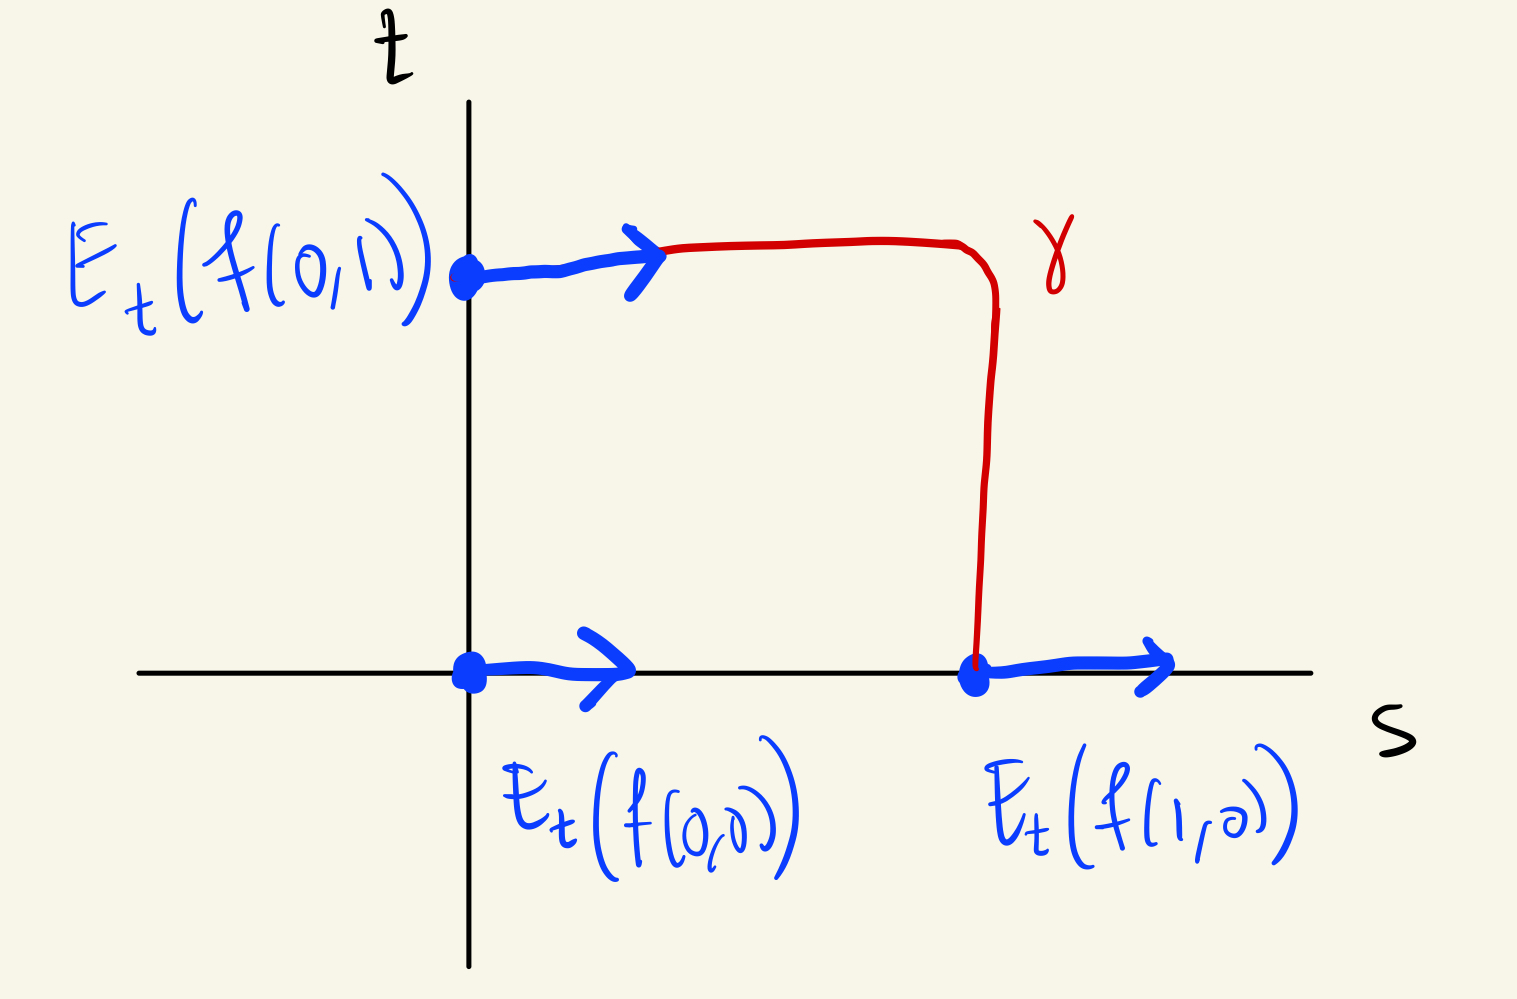
\includegraphics[width=0.5\textwidth]{fig5}
\end{figure}
Esta curva se ve localmente 
\fi\fi\end{proof}
\end{thing6}

\begin{thing6}{Exercício}\label{exer:}\leavevmode
Suponha que \(M\) tem curvatura seccional não-positiva, \(K \leq 0\). Mostre que \(M\) é uma variedade sem pontos conjugados, isto é, para todo \(p \in M\), o conjunto dos pontos conjugados a \(p\) é vazio.
\end{thing6}

\begin{proof}[Solução]\leavevmode
	Suponga que existen dos puntos conjugados \(p\) y \(q\). Es decir, existe una geodésica \(\gamma:(a,b) \to M\) uniendo \(p\) y \(q\), y un campo de Jacobi \(J \in \mathfrak{X}^J_\gamma\) tal que \(J(a)=0\),  \(J(b)=0\).  De acuerdo a las cuentas hechas en aula, sabemos que
\[\|J(t)\|^2=\|w\|^2t^2-\frac{1}{3}K(w,v)t^4+O(t^4)\]
donde \(v=\gamma'(0)\) y \(w=J'(0)\). Evaluando en \(b\) y pasando la curvatura seccional (que es negativa) del lado izquierdo, obtenemos que \(\|w\|^2b^2+O(b^4)\) es un número negativo.

{\color{2}Pregunta:} puedo tener problemas con los términos \(O(b^4)\)? La sugerencia de Manfredo (ex. 5 cap. V) es diferente (también logré seguirla).
\end{proof}
\clearpage
\subsection{Minimizante \(\implies\) geodésica}

\begin{thing4}{Exercício 8}[Curvas minimizantes]\label{exer:8}\leavevmode
\begin{enumerate}[label=(\alph*)]
\item Seja \(\gamma\) uma curva suave por partes parametrizada por comprimento de arco (this is important, velocity is 1) conectando \(p\) a \(q\). Mostre que se \(d(p,q)=\ell(\gamma)\) então \(\gamma\) é uma geodésica.
\end{enumerate}
\end{thing4}

\begin{proof}[Solution]\leavevmode
Imagino que podemos só usar a primeira fórmula da variação:
\[S'(0)=-\int_a^b \left<V,\gamma''\right>dt.\]
(na página que segue anexo uma prova dela, mas isso é extra.)

É claro que se \(\gamma\) é minimizante, estamos num ponto crítico do funcional de distância \(S\), é se cumple a primeira fórmula da variação.

\begin{question}\leavevmode
Para mim parece que daí segue que \(\gamma''=0\), porque a métrica é não degenerada. Porém, \cite{ler}, thm. 6.4 afirma que devemos usar \(V=\gamma''\) para concluir esse exercício. Isso não entendo por que.
\end{question}
\end{proof}

\subsection{First variation formula explained}
\textbf{Explanation of first variation formula.} Não precisa ler :)

Consider a \textit{\textbf{variation}} of \(\gamma\), which is like a homotopy:
\begin{align*}
	\Gamma: (a,b)\times(-\varepsilon,\varepsilon) &\longrightarrow M \\
	\Gamma(t,s) &=\gamma(t)+sV(\gamma(t))
\end{align*}
where \(V \in \mathfrak{X}_\gamma\) is a vector field along \(\gamma\) called the \textit{\textbf{variation field}}, and it has to vanish on the endpoints. Then there's the \textit{\textbf{length functional}} 
\[S(s):=\ell(\Gamma(t,s))=\int_a^b|\nabla_{\frac{d}{dt}}\Gamma(t,s)|dt.\]
Because \(\gamma=\Gamma(t,0)\) is minimizing, we know that \(S'(0)=0\). Then we compute that and hope that it will say \(\gamma''=0\).
\begin{align*}
S'(0)&=\int_a^b\frac{d}{ds}\Big|_{s=0}\left<\nabla_t\Gamma(t,s),\nabla_t\Gamma(t,s)\right>^{1/2}dt\\
&=\int_a^b \frac{\cancel{2}}{\cancel{2}\cancelto{1}{\left|\Gamma(s,t)\right|}}\left<\nabla_s \nabla_t\Gamma(t,s),\nabla_t\Gamma(t,s)\right>dt\\
&\overset{\substack{\text{symmetry}  \\ \text{lemma} }}{=}\int_a^b\left<\nabla_t\underbrace{\nabla_s\Gamma(t,s)}_{=V},\nabla_t\Gamma(t,s)\right>dt\\
&=\int_a^b\frac{d}{dt}\Big|_{t=0}\left<V,\nabla_t\Gamma(t,s)\right>-\int_a^b\left<V,\underbrace{\nabla_t\nabla_t\Gamma(t,s)}_{\gamma''}\right>dt
\end{align*}
and the first one vanished out fundamental theorem of calculus and the fact that \(V\) is zero on the endpoints.

So we get that if \(\gamma\) minimizes distance, this integral is zero for any variation of \(\gamma\).

\begin{thing8}{Remarks}\leavevmode
\begin{itemize}
\item Symmetry lemma basically follows from commutativity of partial derivatives in \(\mathbb{R}^{n}\). Florit used pullback connection (as in the previous exercise!) and \cite{ler} used Christoffel symbols.
\item The true version of the variation formula admits that \(\Gamma\) is only piecewise smooth. The formula becomes less nice and the proof a little more involved, I won't do it, but something nice comes out of that: the fact that you realise that geodesics can't have corners because:
	\begin{figure}[H]
		\centering
		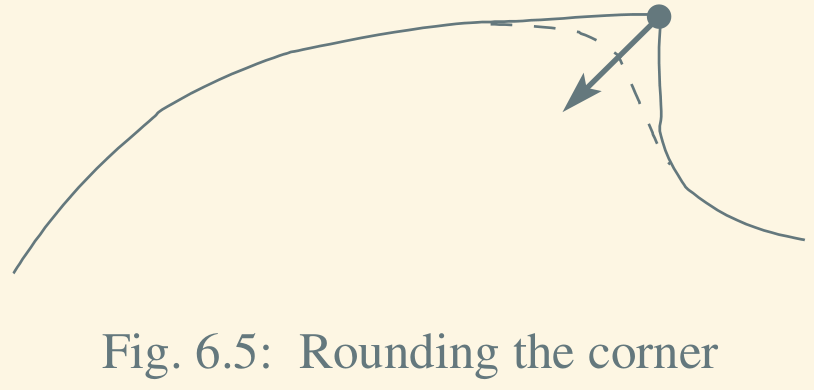
\includegraphics[width=0.3\textwidth]{fig3}
	\end{figure}
	so it would be nice to understand that precisely but \(\mathsf{OK}\).
\end{itemize}
\end{thing8}


\subsection{Duas geodésicas}
Mais um: 

\begin{thing4}{Exercício 8}[Curvas minimizantes]\label{exer:8}\leavevmode
\begin{enumerate}[label=(\alph*)]
	\item[(b)] Suponha que \(\gamma,\sigma:[0,2] \to M\) são geodésicas distintas e satisfazem: \(\gamma(0)=\sigma(0):=p\), \(\gamma(1)=\sigma(1):=q\), \(\gamma\) e \(\sigma\) realizam a distância entre \(p\) e \(q\). Mostre que \(\gamma\) não realiza a distância entre \(p\) e \(\gamma(1+s)\) para nenhum \(s>0\).
\end{enumerate}
\end{thing4}

\begin{proof}\leavevmode
Argumentamos na monitoria que teriamos um problema de diferenciabilidade. Pela explicação dada em  \cite{ler} sobre a suavização de quinas, sabemos que as geodésicas devem ser suaves. Porém, que não poderia acontecer algo assim?
\begin{figure}[H]
	\centering
	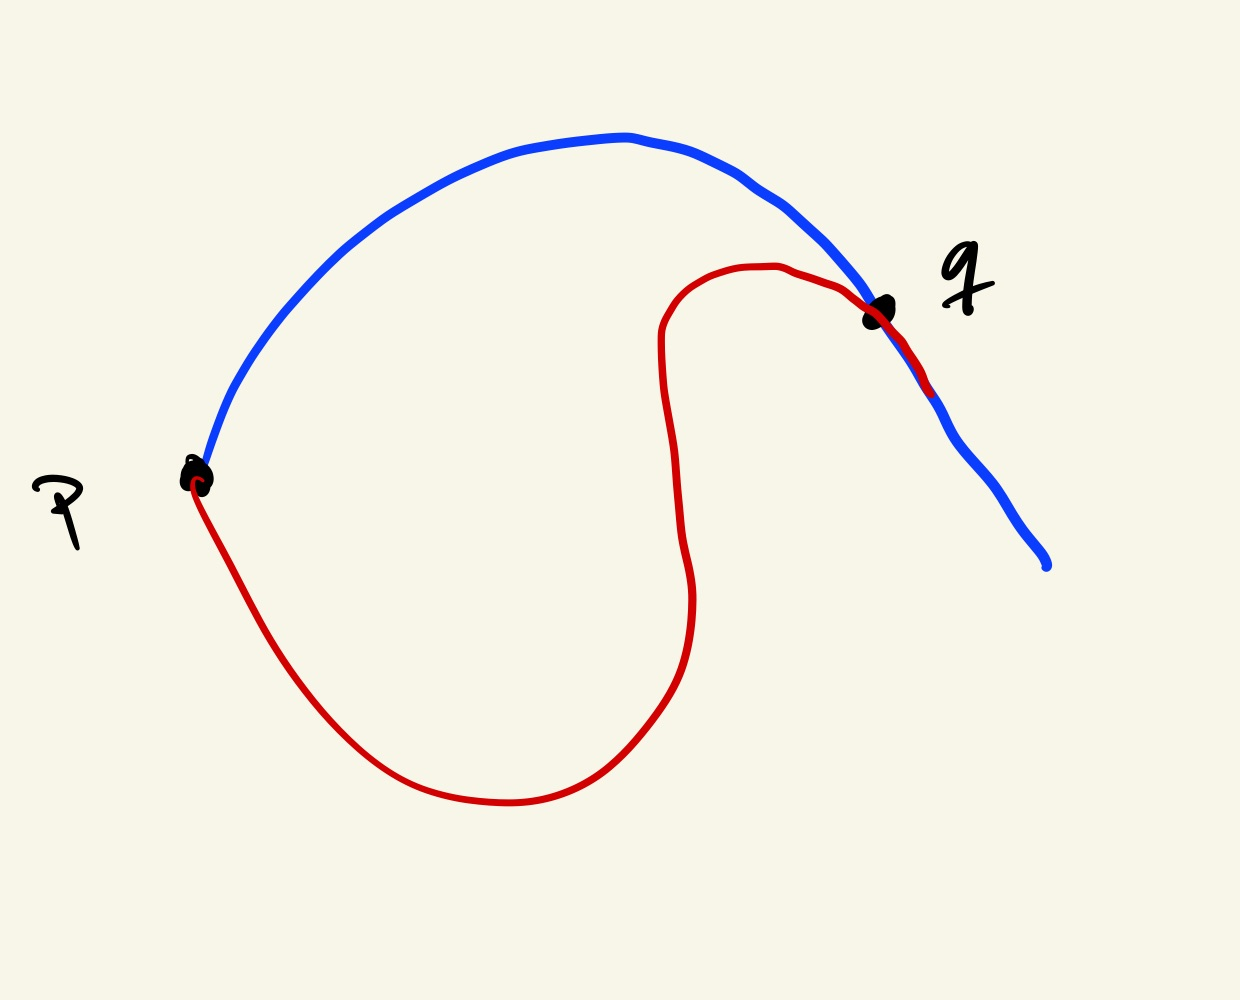
\includegraphics[width=.3\textwidth]{fig2}
\end{figure}
\end{proof}

\begin{exercise}\leavevmode
Show that for a bi-invariant metric on a Lie Group, it holds that \(\operatorname{exp}_e=\operatorname{exp}^G\).
\end{exercise}

\begin{proof}[Solution]\leavevmode
After delving into the abyss of definitions, I think it boils down to showing that \(\nabla_{X_v} X_v=0\), where \(v \in \mathfrak{g}\). So we have to use that the metric is bi-invariant. But it's not necessarily Levi-Civita connection…
\end{proof}

\clearpage

\begin{thing6}{Exercício}\label{exer:}\leavevmode
Seja \(M\) completa, \(S \subset M\) compacta, \(L \subset M\) completa. Mostre que existe uma geodésica minimizante unindo \(S\) e \(L\) (isso é fácil), e que toda geodésica minimizante unindo \(S\) e \(L\) intersecta \(S\) e \(L\) perpendicularmente.

\textbf{Sugestão}
\begin{figure}[H]
	\centering
	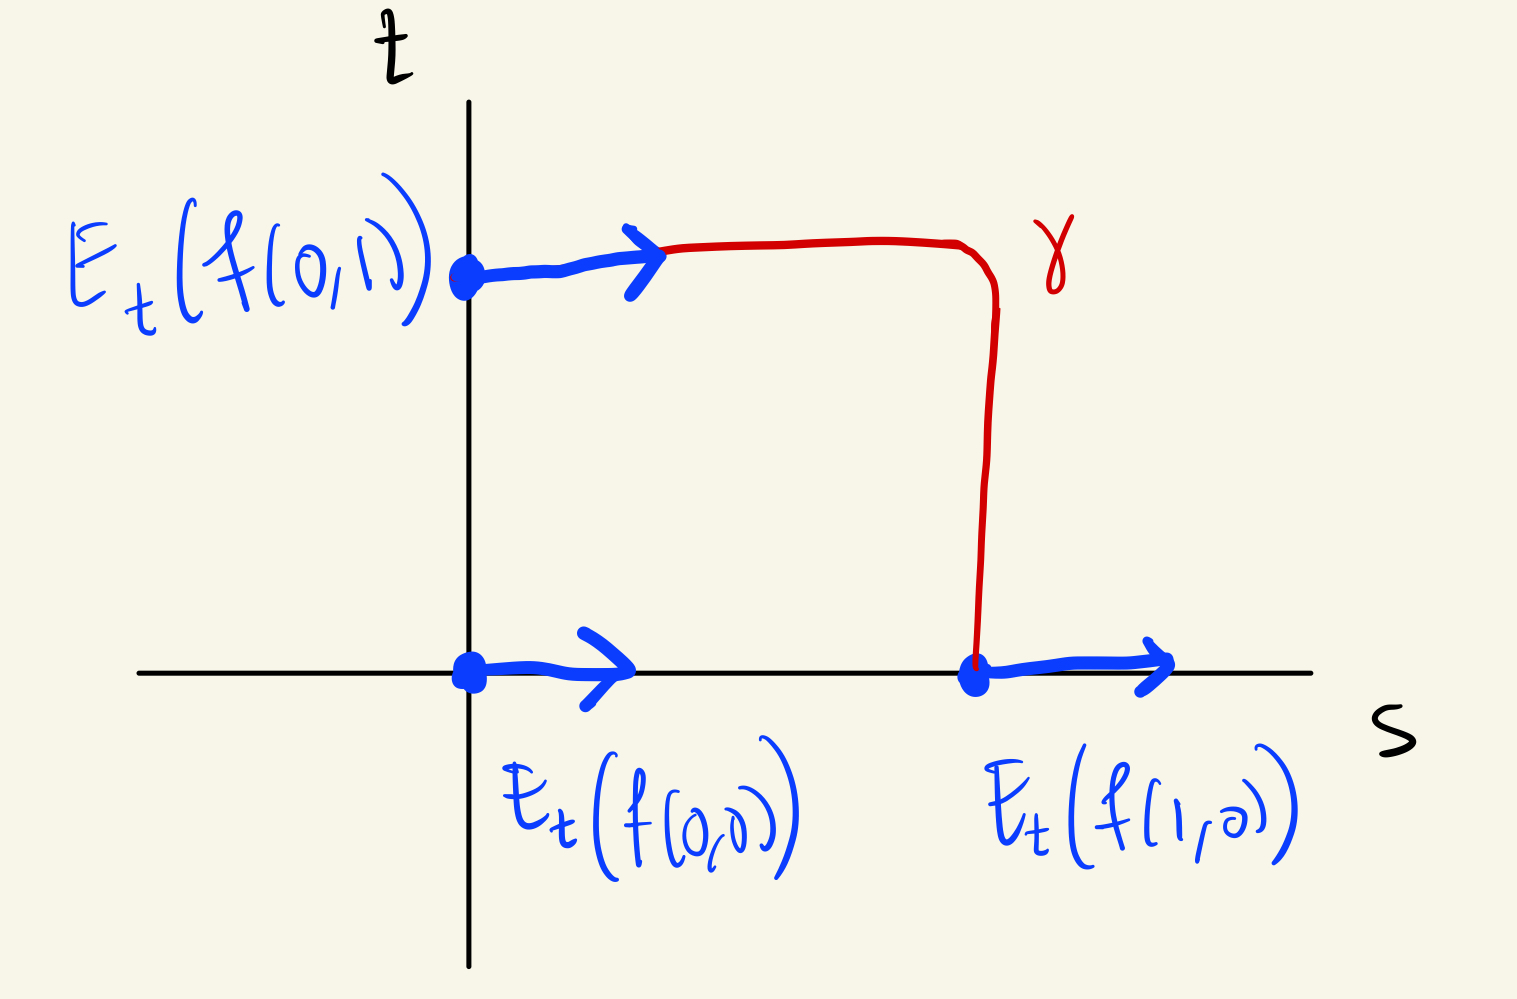
\includegraphics[width=0.5\textwidth]{fig5}
	\caption*{}
\end{figure}
\end{thing6}

\subsection{minimal submanifolds}

Consider an isometric immersion \((M,g) \to(\tilde{M},\tilde{g})\). Let  \(\xi\) be a normal unit vector field---so this only works ``nice" for orientable \(M\); in the nonorientable case you get that the normal section vanishes, and I think the following argument doesn't work. So maybe that's why we'd look for local volume minimizers.

Right so the variation is this:
\begin{align*}
	f: (-\varepsilon,\varepsilon)\times M &\longrightarrow \tilde{M} \\
	f(s,p) &=\operatorname{exp}_{p}(s \xi)
\end{align*}
Then \(f_s:=f(s,\cdot):M \longrightarrow \tilde{M}\) is an immersion (in general not isometric, that's the point) whose image we denote by \(M_s\). Now we define the \textit{\textbf{volume functional}} that simply computes the volume of \(M_s\):
\[S(s):= \int_{M}\operatorname{Vol}_{f_s ^*\tilde{g}}=\int_M f_s^*\operatorname{Vol}_{\tilde{g}}.\]
(\(S\) is physics notation and \(s\) is Florit notation.)

\begin{exercise}\leavevmode
Compute \(S'(0)\).
\end{exercise}
TL;DR. The derivative of the determinant is a trace, that trace is the trace of the shape operator, which is the mean curvature.

\begin{proof}[Solution]\leavevmode
How to express volume in any coordinate system?
\[\sqrt{\det (f^* _sg)_{ij}}dx^1\wedge\ldots\wedge dx^n\]
Let's differentiate:
\begin{align*}
	\frac{d}{ds}S(s)&=\frac{d}{ds}\int_M\operatorname{Vol}_{f^*_s\tilde{g}}=\frac{d}{ds}\int_M \sqrt{\det (f^* _sg)_{ij}}dx^1\wedge\ldots\wedge dx^n\\
&=\int_M \frac{d}{ds}\sqrt{\det (f^* _sg)_{ij}}dx^1\wedge\ldots\wedge dx^n
\end{align*}
And that's as far as normal human beings can get. We ask for help, and find
\iffalse No wait I think I can get farther: what is \(f\)? What is that determinant? Mmm… I think the matrix should be
\[\Big( f^* _s g\Big)_{ij}=\Big(g(f^s_*\partial_i,f^s_* \partial_j\Big)_{ij}\]
\(\mathsf{OK}\) and now yes, what is \(f_s\)? \(f_s(p)=\operatorname{exp}_p(s\xi_p)\)… so it is kind of unclear how to proceed. I think I should take a curve \(\gamma\) that realizes the vector \(\partial_i\) and compose that with the function \(f_s\). gpt claims that this derivative the is
\begin{align*}
f^s_*\partial_i&=\frac{d}{dt}\Big|_{t=0}\operatorname{exp}_{\gamma(t)}(s\xi(\gamma(t))=d_{s\xi(p)}\operatorname{exp}_p\Big(\partial_i + s \nabla_{\gamma'(0)}\xi\Big)
\end{align*}
\(\mathsf{OK}\) moving on. Now I compute the determinant of these things, and realise well, that's nonsense, there should be another way.

So this what normal human beings cannot compute: the square root of the determinant. Actually normal human beings cannot even compute the derivative of the determinant. They use\fi \href{https://en.wikipedia.org/wiki/Jacobi%27s_formula}{wikipedia} article on Jacobi's formula:
	\[\boxed{\frac{d}{dt}\det A(t)=\det A(t) \cdot \operatorname{tr}\left(A(t)^{-1}\cdot \frac{d}{dt}A(t)\right)}\]
and using that we see that
\[\boxed{\frac{d}{dt}\sqrt{\det A(t)} =\frac{1}{2}\sqrt{\det A(t)} \cdot\operatorname{tr}\left(A(t)^{-1}\cdot \frac{d}{dt}A(t)\right) }\]
So we put \(A(s)=(f^*_s\tilde{g})_{ij}\). The good news is that square root of the determinant part is exactly the local coordinate function of \(\operatorname{Vol}_{f_0^*\operatorname{Vol}_{\tilde{g}}}=\operatorname{Vol}_g\) (\(f_0=f\) is an isometric immersion). Then we only have to integrate that other function, which hopefully is related to the mean curvature.

Before computing recall the basic equations of submanifold theory: for \(X,Y \in \mathfrak{X}(M)\), \(\xi \in \Gamma(T^\perp M)\), \(\tilde{\nabla}\) L.C. connection of \(\tilde{M}\) and \(\nabla\) LC connection of \(M\) isometrically immersed in  \(\tilde{M}\), splitting everything into normal and tangent part we get
\[\boxed{\tilde{\nabla}_XY:=\nabla_XY+\alpha(X,Y)}\]
\[\boxed{\tilde{\nabla}_X\xi:=-A_\xi X+\nabla^\perp_X\xi}\]
and call \(\alpha\) the second fundamental form and \(A\) the shape operator. These two equations/definitions together imply
\[\boxed{\left<\xi,\alpha(X,Y)\right>=\left<-A_\xi X,Y\right>}\]


Let's compute
\begin{align*}
\frac{d}{ds}\Big|_{s=0}(f_s^*\tilde{g})_{ij}&=\frac{d}{ds}\Big|_{s=0}f_s^*\tilde{g}\left(\partial_i,\partial_j\right)=\frac{d}{ds}\Big|_{s=0}\tilde{g}(f^s_*\partial_i,f^s_*\partial_j)\\
&=\tilde{g}\left(\nabla_{\partial_s}f^s_*\partial_i,f^s_*\partial_j\right)+\tilde{g}\left(f^s_*\partial_i,\nabla_{\partial_s}f_*^s\partial_j\right)\\
&=\tilde{g}\left(\nabla_{\partial_s}f^0_*\partial_i,f_*^0\partial_j\right)+\tilde{g}\left(f^0_*\partial_i,\nabla_{\partial_s}f_*^0\partial_j\right)\\
&=\tilde{g}\left(f_*\nabla_{\partial_s}\partial_i,\partial_j\right)+\tilde{g}\left(\partial_i,f_* \nabla_{\partial_s}\partial_j\right)\quad \text{\(f=f^0\) isom. imm.}\\
&=\tilde{g}\left(f_*\nabla_{\partial_i}\partial_s,\partial_j\right)+\tilde{g}\left(\partial_i,f_* \nabla_{\partial_j}\partial_s\right)
\end{align*}
Hmmm… the point is that we arrive at the variational field \(\nabla_{\partial_s}f(s,p)=\xi(p)\). If we assume (for now) that \(\xi\) is normal to \(M\) then upon differentiation we get:
\[\nabla_{\partial_i}\xi=-A_{\xi}\partial_i+N\]
where the normal component \(N\) vanishes since it is orthogonal to the basic tangent vectors of \(M\). We conclude that
\begin{align*}
\frac{d}{ds}\Big|_{s=0}(f_s^*\tilde{g})_{ij}&=\tilde{g}\left(-A_{\xi}\partial_i,\partial_j\right)+\tilde{g}\left(\partial_i,-A_{\xi}\partial_j\right)\\
&=\tilde{g}(\xi,\alpha(\partial_i,\partial_j))+\tilde{g}(\alpha(\partial_j,\partial_i),\xi)\\
&=2\tilde{g}(\xi,\alpha(\partial_i,\partial_j))\qquad\qquad \text{\(\alpha\) is symmetric}\\
&=-2\tilde{g}(A_{\xi}\partial_i,\partial_j)
\end{align*}
Now we have to multiply by the inverse matrix, which is just the inverse of the metric in \(M\) because we are at \(s=0\). It turns out that that's how the trace looks like in coordinates, see  \cite{ler} p. 28: if \(h\) is any covariant \(2\)-tensor field,
\[\operatorname{tr}_gh=g^{ij}h_{ij}\]
which is exactly what we are computing! The shape operator, seen as a \((1,1)\)-tensor field has components \(\tilde{g}(A_{\xi}\partial_i,\partial_j)\). So all this time we've been looking at the mean curvature---which is defined as the trace of the shape operator.

But wait a minute didn't you say that the mean curvature is defined as
\[H:=\operatorname{tr}A_{\xi}=\sum_i \tilde{g}(A_{\xi}E_i,E_i)\]
for any orthonormal frame \(E_i\)? And that's the point---\(\partial_i\) need not be orthonormal, and the trace is defined like that in general.

We conclude
\[\frac{d}{ds}\Big|_{s=0}S(s)=-\int_M H \operatorname{Vol}_{g}\]
which says: \textbf{zeroes of the mean curvature function correspond to critical points of the volume functional}.
\end{proof}

\textbf{Addendum.} And the mean curvature vector? The mean curvature vector is \(H\xi\) for unit normal \(\xi\). And \(\tilde{g}(H\xi,\xi)=H\).

\textbf{Questions} 
\begin{itemize}
\item Is the computation of the difficult part correct?
\item What about that part with the inverse and ``the components of the shape operator as a \((1,1)\)-tensor"?
\item \textbf{Why can't we just choose an orthonormal frame and that's it}? 
\end{itemize}

\iffalse
\textbf{Lance:} multiplying by the inverse will give \(\tilde{g}(H,\xi)\) where \(H\) is mean curvature vector:
\[H:=\operatorname{tr}A_{\xi}\cdot\xi=\left(\sum_i \tilde{g}(A_{\xi}\partial_i,\partial_i)\right)\xi\]
for any orthonormal frame \(\partial_i\). So I think I'm aiming to prove that \textit{the trace of the inverse of the pullback metric times the derivative of the pullback metric} gives \[\tilde{g}(H,\xi)=\operatorname{tr}A_\xi \tilde{g}(\xi,\xi)=\operatorname{tr}A_{\xi}\] if \(\xi\) is unit.

Which sounds terribly con



So on the one hand we have the derivative of the pullback metric, whose \((i,j)\)-entry is what we have just computed. On the other hand we have the inverse of the pullback metric, whose \((i,j)\)-entry we may denote by \(g^{ij}_s\). So we have two matrices \(A\) and \(B\)
 \[A_{ij}:=g_s^{ij}\qquad \qquad B_{ij}:=\tilde{g}(\xi,\alpha_{ij})\]
and their product \(C=AB\) has coordinates  \(c_{ij}=\sum_k a_{ik}b_{kj}\).

So first fix \(i,j,k\) and \(\ell\) to simply write
\[(f^* _s\tilde{g})^{k\ell}\tilde{g}\Big(\xi,\alpha(\partial_i,\partial_j)\Big)=(\xi,g^{k \ell}_s\alpha_{ij})\]
Now take trace:
\[\operatorname{tr}=\sum_i \]


… and take trace… But wait who is the mean curvature? It's the trace of \(A\). So
\[H=\sum \tilde{g}(\partial_i,A_{\xi}\partial_i)\]
So if you look at the diagonal over there, you are already computing twice the mean curvature. But you still need to multiply by the inverse… and also what happens with the terms that are not in the diagonal? And also the mean curvature is a number and I think the mean curvature vector is just the unit normal multiplied by the mean curvature.

So \textbf{Question:} after doing my computation of the \textbf{derivative of the pullback metric w.r.t. \(s\)}, I arrive to that formula you had also written. Then what? how do we multiply by the inverse of the pullback metric?
\fi



\subsection{minimal submanifolds good}

Consider an isometric immersion \((M,g) \to(\tilde{M},\tilde{g})\). Let  \(\xi \in\mathfrak{X}(M)\). 

The variation is this:
\begin{align*}
	f: (-\varepsilon,\varepsilon)\times M &\longrightarrow \tilde{M} \\
	f(s,p) &=\operatorname{exp}_{p}(s \xi)
\end{align*}
Then \(f_s:=f(s,\cdot):M \longrightarrow \tilde{M}\) is an immersion (in general not isometric, that's the point) whose image we denote by \(M_s\). Now we define the \textit{\textbf{volume functional}} that simply computes the volume of \(M_s\):
\[S(s):= \int_{M}\operatorname{Vol}_{f_s ^*\tilde{g}}=\int_M f_s^*\operatorname{Vol}_{\tilde{g}}.\]

\begin{exercise}\leavevmode
Compute \(S'(0)\).
\end{exercise}

\begin{proof}[Solution]\leavevmode
How to express volume in any coordinate system?
\[\sqrt{\det (f^* _sg)_{ij}}dx^1\wedge\ldots\wedge dx^n\]
Let's differentiate:
\begin{align*}
	\frac{d}{ds}S(s)&=\frac{d}{ds}\int_M\operatorname{Vol}_{f^*_s\tilde{g}}=\frac{d}{ds}\int_M \sqrt{\det (f^* _sg)_{ij}}dx^1\wedge\ldots\wedge dx^n\\
&=\int_M \frac{d}{ds}\sqrt{\det (f^* _sg)_{ij}}dx^1\wedge\ldots\wedge dx^n
\end{align*}
And that's as far as normal human beings can get. We ask for help, and find
\iffalse No wait I think I can get farther: what is \(f\)? What is that determinant? Mmm… I think the matrix should be
\[\Big( f^* _s g\Big)_{ij}=\Big(g(f^s_*\partial_i,f^s_* \partial_j\Big)_{ij}\]
\(\mathsf{OK}\) and now yes, what is \(f_s\)? \(f_s(p)=\operatorname{exp}_p(s\xi_p)\)… so it is kind of unclear how to proceed. I think I should take a curve \(\gamma\) that realizes the vector \(\partial_i\) and compose that with the function \(f_s\). gpt claims that this derivative the is
\begin{align*}
f^s_*\partial_i&=\frac{d}{dt}\Big|_{t=0}\operatorname{exp}_{\gamma(t)}(s\xi(\gamma(t))=d_{s\xi(p)}\operatorname{exp}_p\Big(\partial_i + s \nabla_{\gamma'(0)}\xi\Big)
\end{align*}
\(\mathsf{OK}\) moving on. Now I compute the determinant of these things, and realise well, that's nonsense, there should be another way.

So this what normal human beings cannot compute: the square root of the determinant. Actually normal human beings cannot even compute the derivative of the determinant. They use\fi \href{https://en.wikipedia.org/wiki/Jacobi%27s_formula}{wikipedia} article on Jacobi's formula:
	\[\boxed{\frac{d}{dt}\det A(t)=\det A(t) \cdot \operatorname{tr}\left(A(t)^{-1}\cdot \frac{d}{dt}A(t)\right)}\]
and using that we see that
\[\boxed{\frac{d}{dt}\sqrt{\det A(t)} =\frac{1}{2}\sqrt{\det A(t)} \cdot\operatorname{tr}\left(A(t)^{-1}\cdot \frac{d}{dt}A(t)\right) }\]
But admittedly that is cheating so here's how to compute the derivative of the determinant. We write
\[A(t)=A+tB+\mathcal{O}(t^2)=A(\operatorname{Id}+tA^{-1}B+\mathcal{O}(t^2))=A(t^{-1}\operatorname{Id}+A^{-1}B+\mathcal{O}(t^2))\]
I think this is the Taylor expansion of the smooth function \(A(t)\), done entry by entry. We did the two other manipulations because we remembered the characteristic polynomial, which I think is the determinant of \(C-t \operatorname{Id}\). Suppose we can diagonalize \(C=A^{-1}B\). Then tj


So we put \(A(s)=(f^*_s\tilde{g})_{ij}\). The good news is that square root of the determinant part is exactly the local coordinate function of \(\operatorname{Vol}_{f_0^*\operatorname{Vol}_{\tilde{g}}}=\operatorname{Vol}_g\) (\(f_0=f\) is an isometric immersion). Then we only have to integrate that other function, which hopefully is related to the mean curvature.

Before computing recall the basic equations of submanifold theory: for \(X,Y \in \mathfrak{X}(M)\), \(\xi \in \Gamma(T^\perp M)\), \(\tilde{\nabla}\) L.C. connection of \(\tilde{M}\) and \(\nabla\) LC connection of \(M\) isometrically immersed in  \(\tilde{M}\), splitting everything into normal and tangent part we get
\[\boxed{\tilde{\nabla}_XY:=\nabla_XY+\alpha(X,Y)}\]
\[\boxed{\tilde{\nabla}_X\xi:=-A_\xi X+\nabla^\perp_X\xi}\]
and call \(\alpha\) the second fundamental form and \(A\) the shape operator. These two equations/definitions together imply
\[\boxed{\left<\xi,\alpha(X,Y)\right>=\left<-A_\xi X,Y\right>}\]


Let's compute
\begin{align*}
\frac{d}{ds}\Big|_{s=0}(f_s^*\tilde{g})_{ij}&=\frac{d}{ds}\Big|_{s=0}f_s^*\tilde{g}\left(\partial_i,\partial_j\right)=\frac{d}{ds}\Big|_{s=0}\tilde{g}(f^s_*\partial_i,f^s_*\partial_j)\\
&=\tilde{g}\left(\nabla_{\partial_s}f^s_*\partial_i,f^s_*\partial_j\right)+\tilde{g}\left(f^s_*\partial_i,\nabla_{\partial_s}f_*^s\partial_j\right)\\
&=\tilde{g}\left(\nabla_{\partial_s}f^0_*\partial_i,f_*^0\partial_j\right)+\tilde{g}\left(f^0_*\partial_i,\nabla_{\partial_s}f_*^0\partial_j\right)\\
&=\tilde{g}\left(f_*\nabla_{\partial_s}\partial_i,\partial_j\right)+\tilde{g}\left(\partial_i,f_* \nabla_{\partial_s}\partial_j\right)\quad \text{\(f=f^0\) isom. imm.}\\
&=\tilde{g}\left(f_*\nabla_{\partial_i}\partial_s,\partial_j\right)+\tilde{g}\left(\partial_i,f_* \nabla_{\partial_j}\partial_s\right)
\end{align*}
Hmmm… the point is that we arrive at the variational field \(\nabla_{\partial_s}f(s,p)=\xi(p)\), which upon differentiation gives:
\[\nabla_{\partial_i}\xi=-A_{\xi}\partial_i+N\]
where the normal component \(N\) vanishes since it is orthogonal to the basic tangent vectors of \(M\). We conclude that
\begin{align*}
\frac{d}{ds}\Big|_{s=0}(f_s^*\tilde{g})_{ij}&=\tilde{g}\left(-A_{\xi}\partial_i,\partial_j\right)+\tilde{g}\left(\partial_i,-A_{\xi}\partial_j\right)\\
&=\tilde{g}(\xi,\alpha(\partial_i,\partial_j))+\tilde{g}(\alpha(\partial_j,\partial_i),\xi)\\
&=2\tilde{g}(\xi,\alpha(\partial_i,\partial_j))\qquad\qquad \text{\(\alpha\) is symmetric}\\
&=-2\tilde{g}(A_{\xi}\partial_i,\partial_j)
\end{align*}
Now we have to multiply by the inverse matrix, which is just the inverse of the metric in \(M\) because we are at \(s=0\). It turns out that that's how the trace looks like in coordinates, see  \cite{ler} p. 28: if \(h\) is any covariant \(2\)-tensor field,
\[\operatorname{tr}_gh=g^{ij}h_{ij}\]
which is exactly what we are computing! The shape operator, seen as a \((1,1)\)-tensor field has components \(\tilde{g}(A_{\xi}\partial_i,\partial_j)\). So all this time we've been looking at the mean curvature---which is defined as the trace of the shape operator.

But wait a minute didn't you say that the mean curvature is defined as
\[H:=\operatorname{tr}A_{\xi}=\sum_i \tilde{g}(A_{\xi}E_i,E_i)\]
for any orthonormal frame \(E_i\)? And that's the point---\(\partial_i\) need not be orthonormal, and the trace is defined like that in general.

We conclude
\[\frac{d}{ds}\Big|_{s=0}S(s)=-\int_M H \operatorname{Vol}_{g}\]
which says: \textbf{zeroes of the mean curvature function correspond to critical points of the volume functional}.
\end{proof}

\textbf{Addendum.} And the mean curvature vector? The mean curvature vector is \(H\xi\) for unit normal \(\xi\). And \(\tilde{g}(H\xi,\xi)=H\).

\textbf{Questions} 
\begin{itemize}
\item Is the computation of the difficult part correct?
\item What about that part with the inverse and ``the components of the shape operator as a \((1,1)\)-tensor"?
\item \textbf{Why can't we just choose an orthonormal frame and that's it}? 
\end{itemize}

\iffalse
\textbf{Lance:} multiplying by the inverse will give \(\tilde{g}(H,\xi)\) where \(H\) is mean curvature vector:
\[H:=\operatorname{tr}A_{\xi}\cdot\xi=\left(\sum_i \tilde{g}(A_{\xi}\partial_i,\partial_i)\right)\xi\]
for any orthonormal frame \(\partial_i\). So I think I'm aiming to prove that \textit{the trace of the inverse of the pullback metric times the derivative of the pullback metric} gives \[\tilde{g}(H,\xi)=\operatorname{tr}A_\xi \tilde{g}(\xi,\xi)=\operatorname{tr}A_{\xi}\] if \(\xi\) is unit.

Which sounds terribly con



So on the one hand we have the derivative of the pullback metric, whose \((i,j)\)-entry is what we have just computed. On the other hand we have the inverse of the pullback metric, whose \((i,j)\)-entry we may denote by \(g^{ij}_s\). So we have two matrices \(A\) and \(B\)
 \[A_{ij}:=g_s^{ij}\qquad \qquad B_{ij}:=\tilde{g}(\xi,\alpha_{ij})\]
and their product \(C=AB\) has coordinates  \(c_{ij}=\sum_k a_{ik}b_{kj}\).

So first fix \(i,j,k\) and \(\ell\) to simply write
\[(f^* _s\tilde{g})^{k\ell}\tilde{g}\Big(\xi,\alpha(\partial_i,\partial_j)\Big)=(\xi,g^{k \ell}_s\alpha_{ij})\]
Now take trace:
\[\operatorname{tr}=\sum_i \]


… and take trace… But wait who is the mean curvature? It's the trace of \(A\). So
\[H=\sum \tilde{g}(\partial_i,A_{\xi}\partial_i)\]
So if you look at the diagonal over there, you are already computing twice the mean curvature. But you still need to multiply by the inverse… and also what happens with the terms that are not in the diagonal? And also the mean curvature is a number and I think the mean curvature vector is just the unit normal multiplied by the mean curvature.

So \textbf{Question:} after doing my computation of the \textbf{derivative of the pullback metric w.r.t. \(s\)}, I arrive to that formula you had also written. Then what? how do we multiply by the inverse of the pullback metric?
\fi

\subsection{ponto focal hipersuperfície}

\(M^n \subset \mathbb{R}^{n+1}\) hipersuperfície. Calcule os pontos focais em função das curvaturas principais de \(M\).

\textit{collect your knowledge}. \(q \in \mathbb{R}^{n+1}\) es el punto focal. \(\gamma\) geodesic joining \(p \in M^n\) and \(q\). So it's a geodesic in \(\mathbb{R}^{n+1}\), it must be \(\gamma(t)=(1-t)p+tq\). \(\gamma'(0) \perp M\). A Jacobi field \(J \in \mathfrak{X}^J_\gamma\). So it's a Jacobi field in \(\mathbb{R}^{n+1}\), it must be of the form \(J(t)=tu+v\) for some \(u,v \in \mathbb{R}^{n+1}\). And finally, for \(q\) to be a \textit{\textbf{focal point}} we require that
\begin{align*}
\boxed{J'(0)+A_{\gamma'(0)}J(0)\in T^{\perp}_pM,\qquad \text{and} \qquad \qquad J(r)=0 }
\end{align*}
for some \(r\).

\subsection{pontos focais da esfera}

Calcule os pontos focais de \(S^n \subset S^{n+1}\)

\subsection{distance and second variation}

\begin{thing6}{Exercício}\label{exer:}\leavevmode
Show that \(d(\gamma_v(t),\gamma_w(t))=\|v-w\|t+O(t^2)\). Suggestion: consider the variation given by minimizing geodesics joining \(\gamma_v(t)\) and \(\gamma_w(t)\) for each small \(t\), differentiate.
\end{thing6}

\subsection{lema do índice}

\begin{thing6}{Exercício }\label{exer:}\leavevmode
reescreva a prova do lema do índice usando o tensor \(\overline{J}\) instead of \(J\).
\end{thing6}

\begin{thing6}{lema do índice}\leavevmode
\[\boxed{I_a(V,V) \geq I_a(J,J)}\]
onde \(J\) é de jacobi e \(V\) é 
\end{thing6}

\begin{proof}\leavevmode
FAZER!
\end{proof}

\subsection{sturm y rauch}

\begin{thing6}{Exercício }\label{exer:}\leavevmode
Prove Sturm usando Rauch.
\end{thing6}

\begin{thing6}{Exercício }\label{exer:}\leavevmode
continua que preserva distancia es diferenciable
\end{thing6}

\begin{thing6}{Exercício brutal}\label{exer:brutal}\leavevmode

\end{thing6}
\section{Monitorias}

\subsection{Abril 25}
\begin{thing6}{Kobayashi theorem}[Also \cite{pet} prop. 5.6.5]\label{exer:}\leavevmode
\(\sigma:M \to M\) isometria.
Prove que cada componente conexa do conjunto dos pontos fixos de \(\sigma\) é uma subvariedade totalmente geodésica.
\end{thing6}

\begin{proof}[Solução]\leavevmode
Primeiro mostramos que os pontos fixos de \(\sigma\), \(M^\sigma\) tem estrutura de subvariedade. Pegue uma bola geodésica \(B_\varepsilon(p)\) e um ponto \(q \in B_\varepsilon(p)\). Existe um vetor \(v \in B_\varepsilon(0) \subset T_pM\) tal que \(\operatorname{exp}_p(v)=q\). Então \(q\) tem coordenadas \(v\) porque
 \[\underbrace{\operatorname{exp}^{-1}_p}_{\text{carta} }(\underbrace{\operatorname{exp}_p(v)}_{q})=v\]
Agora aplique \(d_p\sigma\). Aqui usamos o diagrama de naturalidade da exponencial:
\[\begin{tikzcd}
	B_\varepsilon(0)\subset T_pM\arrow[r,"d_p\sigma"]\arrow[d,"\operatorname{exp}_p",swap]&B_\varepsilon(0) \subset T_pM\arrow[d,"\operatorname{exp}_p"]\\
	B_\varepsilon(p)\subset M\arrow[r,swap,"\sigma"]&B_\varepsilon(p) \subset M
\end{tikzcd}\]
esse diagrama comuta se \(\sigma\) é uma isometria. 

Lembre por que esse diagrama comuta: por um lado, como \(\sigma\) é isometria, \((\sigma \circ \operatorname{exp}_p)(tv)\) é uma geodésica. Por outro lado, por definição da exponencial, \((\operatorname{exp}_p \circ d_p\sigma)(tv)\) também é uma geodésica. Então basta ver que essas duas geodésicas são a solução da mesma EDO (a condição inicial é a mesma: que as curvas começam em \(p\), claro, pois \(p\) é ponto fixo). Então derive cada uma delas em \(t=0\):
\begin{align*}
\frac{d}{dt}\Big|_{t=0}(\sigma \circ& \operatorname{exp}_p)(tv)=d_{\operatorname{exp}_p(0)}\sigma\cdot d_{0}\operatorname{exp}_p(v)=d_p\sigma \operatorname{Id}(v)\\&=\operatorname{Id} d_p\sigma(v)=d_0 \operatorname{exp}_p d_p\sigma(v)=\frac{d}{dt}\Big|_{t=0}(\operatorname{exp}_p \circ d_p\sigma)(tv)
\end{align*}
O fato do diagrama comutar significa que
\begin{align*}
	\operatorname{exp}_p(d_p\sigma(v))&=\sigma(\operatorname{exp}_p(v))=\sigma(q)\end{align*}
Note que se \(d_p\sigma\) fixa \(v\), automáticamente \(\sigma\) fixa \(q\). Mas ainda, se \(q\) é um ponto fixo de \(\sigma\), aplicando \(\operatorname{exp}_p^{-1}\) obtemos que
\begin{align*}
d_p\sigma(v)&=\operatorname{exp}^{-1}_p(\sigma(q))=\operatorname{exp}^{-1}_p(q)=v
\end{align*}
ou seja, \(d_p\sigma\) fixa \(v\). Isso significa que o conjunto de pontos fixos está em bijeção com os vetores que \(d_p\sigma\) fixa. Em particular o conjunto de pontos fixos de \(\sigma\) está localmente parametrizado como o subespaço vetorial de \(T_pM\) dos pontos fixos de \(d_p\sigma\), ou seja, tem cartas de subvariedade.

Mas ainda, considerando a geodésica \(\gamma(t)=\operatorname{exp}_p(tv)\), como
	\begin{align*}d_p\sigma(tv)=td_p\sigma(v)=tv
\end{align*}
o mesmo argumento mostra que \(\sigma(\gamma(t))=\gamma(t)\). Ou seja, \(\sigma\) fixa toda a geodésica que liga \(p\) e \(q\) desde que fixe qualquer ponto nela. Isso conclui a prova: se \(M^\sigma \cap B_\varepsilon(p)=\{p\}\), pronto! \(\{p\}\) já é uma subvariedade totalmente geodésica.
\end{proof}

\begin{thing4}{Exercício 2}[\cite{pet}]\label{exer:}\leavevmode
\(F:(M,g) \to (M,g)\) conexa, \(F\) isometria, \(p \in M\). Prove que
\[DF_p=-\operatorname{Id}|_{T_pM} \iff \begin{cases}
	F^2=\operatorname{Id}_M\qquad & \\
	p\text{ é ponto fixo isolado} \qquad &
\end{cases}\]
\end{thing4}

\begin{thing4}{Exercício 3}[Petersen]\label{exer:3}\leavevmode
\(N_1,N_2 \subset M\) totalmente geodésicas. Prove que cada componente conexa de \(N_1 \cap N_2\) é uma subvariedade totalmente geodésica.
\end{thing4}

\begin{thing4}{Exercício 4}\label{exer:4}\leavevmode
Que se tem uma superfície (dimensão 2 só!) com um plano de simetria no sentido de que pode reflexar nela, então a curva que essa reflexão fixa é geodésica. Ou seja: se tem uma isometria que não é a identidade
\end{thing4}

\begin{thing4}{Exercício 0}\label{exer:0}\leavevmode
Curvatura negativa implica que…?
\end{thing4}


\subsection{21 maio}

\begin{thing6}{Exercício -1}\label{exer:-1}\leavevmode
Para \((M,g_M)\) e \((N,g_N)\) e \(f:M \to \mathbb{R}_+\), definimos o \textit{\textbf{warped product}} como sendo o produto cartesiano \(M\times N\) com a métrica \(g_M+f^2g_N\).

Se os fatores são completos o warped product é completo.
\end{thing6}

\begin{thing6}{Exercício 0}\label{exer:0}\leavevmode
\(M\) completa, \(K \subset M\) compacto, \(\operatorname{Ric}\geq  \varepsilon>0\) em \(M\setminus K\), então \(M\) completa. Estime o diâmetro de \(M\).
\end{thing6}

\begin{thing6}{Exercício 1}\label{exer:1}\leavevmode
Troque \(\operatorname{s c a l}\) por \(K_M\) no statement de teo. Hadamard. Prove que não da. (Também não da trocando por \(\operatorname{Ric}\), isso é mais difícil de ver.)
\end{thing6}

\begin{thing6}{Exercício 2}\label{exer:2}\leavevmode
\((M^n,g)\) completa, \(\operatorname{Ric}_M>0\). \(A,B\) hipersuperfícies mínimas completas (i.e. traço da segunda forma é zero). Então \(A \cap B \neq  \varnothing\). 
\end{thing6}

\subsection{4 junho}

\begin{exercise}\leavevmode
calcule o diâmetro de \(S^2, \mathbb{T}^2,\mathbb{R}P^{2}\).
\end{exercise}

\clearpage
\section{Exercícios das listas (não entregue)}

\subsection{Lista 3}
\subsubsection{Complemento}

\begin{thing6}{Exercício 21}[Geodésicas e conexões afins]\label{exer:21}\leavevmode
\begin{enumerate}[label=(\alph*)]
\item Seja \(\gamma:I \to M\) uma curva regular definida sobre um intervalo aberto \(I \subset \mathbb{R}\). Prove que \(\gamma\) é uma reparametrização deuma geodésica se e somente se existe \(f:I \to \mathbb{R}\) suave tal que
	\[\nabla_{\frac{d}{dt}}^\gamma \gamma'=f(t)\gamma'\]
	para todo \(t \in I\).
\item Seja \(\nabla\) uma conexão afim em \(M\). Prove que existe uma conexão \(\overline{\nabla}\) em \(M\) que é livre de torção e admite as mersmas geodésicas que \(\nabla\). Há unicidade?
\item Sejam \(\nabla\) e \(\overline{\nabla}\) conexões afins em \(M\), livres de torção. Mostre que \(\nabla\) e \(\overline{\nabla}\) possuem as mesmas geodésicas (a menos de reparametrizações) se e somente se existe uma 1-forma \(\omega\) tal que
	\[\nabla_XY-\overline{\nabla}_XY=\omega(X)Y+\omega(Y)X\]
	para todo \(X,Y \in \mathfrak{X}(M)\).
\end{enumerate}
\end{thing6}

\begin{proof}[Solução]\leavevmode
\begin{enumerate}[label=(\alph*)]
\item (\(\implies\)) Suponha que \(\gamma=\tilde{\gamma} \circ u\) para alguma geodésica \(\tilde{\gamma}\) e \(u:J \to I\) onde \(J\) é outro intervalo aberto.
	\begin{align*}
	\nabla_{\frac{d}{dt}}^\gamma \gamma'&=\nabla^\gamma_{\frac{d}{dt}}(\tilde{\gamma}\circ u)'=\nabla^\gamma_{\frac{d}{dt}}(\tilde{\gamma}'\circ u)u'\\
	&=\frac{d}{dt}u' \tilde{\gamma}'\circ u+u'\nabla^\gamma_{\frac{d}{dt}}\tilde{\gamma}' \circ u
	\end{align*}
	Para aplicar tudo que você sabe de conexões respire fundo e escreva:
	\begin{align*}
	\nabla^\gamma_{\frac{d}{dt}}\tilde{\gamma} \circ u&=\nabla^{\tilde{\gamma}\circ u}_{\frac{d}{dt}}\tilde{\gamma}\circ u\qquad \text{porque \(\gamma=\tilde{\gamma}\circ u\)} \\
	&=(\nabla^{\tilde{\gamma}})^u_{\frac{d}{dt}}\tilde{\gamma}\circ u\qquad\qquad  \text{exercício \#475}\\
	&=\nabla^{\tilde{\gamma}}_{u_*\frac{d}{dt}}\tilde{\gamma}\qquad\qquad  \text{tudo que eu sei} \\
	&=\nabla^{\tilde{\gamma}}_{u'\frac{d}{dt}\circ u}\tilde{\gamma}\qquad\qquad  \text{posso explicar}\\
	&=u'\nabla^{\tilde{\gamma}}_{\frac{d}{dt}\circ u}\tilde{\gamma}
	\end{align*}
	Ah, é porque para qualquer função \(g \in \mathcal{F}(M)\),
	\[\left(u_* \frac{d}{dt}\right)_tg=\frac{d}{dt}\Big|_{t}(g \circ u)=g'(u(t))u'(t)=u'(t) \frac{d}{dt}\Big|_{u(t)}g\]
	So you may want to always remember that
\[\boxed{\nabla^{\tilde{\gamma}\circ u}_{\frac{d}{dt}}(\tilde{\gamma}\circ u)'=u''\tilde{\gamma}'\circ u+(u')^2\nabla^{\tilde{\gamma}}_{\frac{d}{dt}\circ u}\tilde{\gamma}'}\]
Clearly if \(\tilde{\gamma}\) is a geodesic we get the desired result.

\item For the converse we do this: suppose there is a function \(f:I \to \mathbb{R}\) such that \(\nabla^\gamma_{\frac{d}{dt}}\gamma'=f(t)\gamma'\). I want to prove \(\gamma\) is of the form \(\gamma=\tilde{\gamma}\circ u\) for some \(\tilde{\gamma}\) and function \(u\). But hey, if they existed (who could tell?) they would satisfy the equation in that box over there.
\end{enumerate}
\end{proof}

\subsection{Lista 4}
\clearpage
\subsubsection{Mean curvature}

\begin{thing4}{Exercício 8}\label{exer:8}\leavevmode
Seja \((M,g)\) uma variedade Riemanniana. Suponha que existe \(f \in C^\infty(M)\) tal que \(0 \in \mathbb{R}\) é um valor regular e seja \(\Sigma:=f^{-1}(0)\).
\begin{enumerate}[label=(\alph*)]
\item Seja \(N=\frac{\nabla f}{|\nabla f|}\in \mathfrak{X}^\perp(\Sigma)\). Mostre que
	\[\left<\alpha_{\Sigma}(X,Y),N\right>=-\frac{\mathsf{Hess}(f)(X,Y)}{|\nabla f|}\]
para todos \(X,Y \in \mathfrak{X}(\Sigma)\). (Aqui \(\alpha\) é a segunda forma fundamental de \(\Sigma\).)
\item Mostre que a curvatura média de \(\Sigma\) (definida como o traço do operador de forma \(A\)) é dada por
	\[H_\Sigma=-\frac{1}{n}\operatorname{div}\left(\frac{\nabla f}{|\nabla f|}\right) \]
\end{enumerate}
\end{thing4}

\begin{proof}[Solução]\leavevmode
\begin{enumerate}[label=(\alph*)]
\item On one hand,
	\[\left<\alpha(X,Y),\nabla f\right>=-\left<Y,A_{\nabla f}X\right>\]
	and on the other, 
\[\mathsf{Hess}(f)(X,Y)=\left<\widetilde{\nabla}_X\nabla f,Y\right>=\left<-A_{\nabla f}X+\nabla^\perp_X \nabla f,Y\right>\]
then multiply by \(\frac{1}{|\nabla f|}\). (\(\tilde{\nabla}\) é a conexão LC da variedade ambiente.)
\item Para calcular a divergência como o traço do gradiente precisamos de uma base ortonormal de \(M\). Pegue uma base ortonormal \(E_i\) de \(\Sigma\) e agregue \(\frac{\nabla}{|\nabla f|}\). Então temos:
	\begin{align*}
	\operatorname{div}\left(\frac{\nabla f}{|\nabla f|}\right)&=\sum \left<\widetilde{\nabla}_{E_i}\frac{\nabla f}{| \nabla f|},E_i\right>+\underbrace{\left<\widetilde{\nabla}_{\frac{\nabla f}{|\nabla f|}}\frac{\nabla f}{| \nabla f|}, \frac{ \nabla f}{| \nabla f|}\right>}_{=\frac{1}{2}\frac{d}{dt}|\nabla f|^2=0 }\\
	&=\sum \left<- A_{\frac{\nabla f}{| \nabla f|}}E_i,E_i\right>\\
	&=-\operatorname{tr}(X \mapsto A_{\frac{\nabla f}{| \nabla f|}}X)=-nH_{\Sigma}(p)
	\end{align*}
\end{enumerate}
\end{proof}

\clearpage
\section{Lista 1}

\subsection{Revisão}

\begin{thing4}{Exercício 1}\label{exer:1}\leavevmode
Dada uma subvariedade \(M \subseteq \tilde{M}\) uma subvariedade mergulhada e \(X \in \mathfrak{X}(M)\). Mostre que existe um aberto \(U \subset \tilde{M}\) contendo \(M\) e um campo \(\tilde{X} \in \mathfrak{X}(U)\) tal que \(\tilde{X}|_{M}=X\). Caso \(M\) seja subconjunto fechado de \(\tilde{M}\), prove que \(U\) pode ser tomado igual a \(\tilde{M}\). Se \(M\) não é subconjunto fechado de \(\tilde{M}\), pode não existir extensão de \(X\) definida em todo \(\tilde{M}\).
\end{thing4}

\begin{proof}[Solução]\leavevmode
Acho que a prova canônica é tomar coordenadas de subvariedade de \(M \subset \tilde{M}\), i.e. onde \(M\) está dada localmente como o lugar onde se anulam as últimas \(n-m\) funções coordenadas. 

Pegamos uma vizinhança rectificante \(U\) de \(X\) em \(p \in M\), i.e. \(X=\partial_1\) em \(U\). Daí pega para cada vetor normal a exponencial, que percorre pela geodésica um pouqinho. Isso da uma vizinhança em \(\tilde{M}\)…
\end{proof}

\begin{thing4}{Exercício 2}\label{exer:2}\leavevmode
	Seja \(f:M^n \to N^m\) um mapa suave. Os campos \(X \in \mathfrak{X}(M)\) e \(\tilde{X} \in \mathfrak{X}(N)\) são ditos \(f\)-relacionados se \(df_pX_p=\tilde{X}_{f(p)}\), \(\forall  p \in M\). Mostre que se os campos \(X,Y \in \mathfrak{X}(M)\) são, respetivamente, \(f\)-relacionados com \(\tilde{X},\tilde{Y} \in \mathfrak{X}(N)\) então \([X,Y]\) é \(f\)-relacionado com \([\tilde{X},\tilde{Y}]\).
\end{thing4}

\begin{proof}[Solução]\leavevmode
	\textbf{Intento 2.} \(s_1 \in \Gamma(\tau_N)\) está \textit{\textbf{\(f\)-relacionado}} com \(s \in \Gamma(\tau_M)\) se \(s=s_1\oplus s^\perp\) para algum \(s^\perp\in\nu\). Queremos ver que se \(s\overset{f}{\sim}s_1\) e \(t \overset{f}{\sim}t_1\), \([s,t]\overset{f}{\sim}[s_1,t_1]\), ou seja \([s,t]=[s_1,t_1]\oplus [s,t]^\perp\) onde \([s,t]^\perp\) é um vetor em \(\nu\) cuja cara não  é muito importante.
	\begin{align*}
		[s,t]&=[s_1\oplus s^\perp,t_1\oplus t^\perp]=[s_1,t_1]+\underbrace{[s_1,t^\perp]}_{=0}+\underbrace{[s^\perp,t_1]}_{=0}+\underbrace{[s^\perp,t^\perp]}_{\in \nu}
	\end{align*}
{\color{4}Falta un argumentín para ver que esos colchetes se anulan…}

\textbf{Intento 1 (incompleto).} Pegue \(p \in M\). Queremos ver que
\[(f_{*}[X,Y])_p\overset{\text{quero}}{=}[\tilde{X},\tilde{Y}]_{f(p)}.\]
Pegue \(g \in \mathcal{F}(N)\).
\begin{align*}
	[\tilde{X},\tilde{Y}]_{f(p)}&\overset{\operatorname{def}}{=}\tilde{X}_{f(p)}(\tilde{Y}g)-\tilde{Y}_{f(p)}(\tilde{X}g)\\
	&\overset{\operatorname{hip}}{=}f_{*,p}(X_p)(\tilde{Y}g)-f_{*,p}(Y_p)(\tilde{X}g)\\
	&=X_{p}\Big((\tilde{Y}g)\circ f\Big)-Y_p\Big((\tilde{X}g)\circ f\Big)\\
	&\overset{\operatorname{hip}}{=}X_p\Big(\big(f_{*,p}(Y)\big)g\circ f)\Big)-Y_p\Big(\big(f_{*,p}(X_p)\big)g \circ f\Big)\\
\end{align*}
\end{proof}

\begin{thing4}{Exercício 3}\label{exer:3}\leavevmode
Seja \(\pi:M \to N\) uma submersão sobrejetiva. Dado \(Y \in \mathfrak{X}(N)\), mostre que existe \(X \in \mathfrak{X}(M)\) tal que \(X\) é \(\pi\)-relacionado com \(Y\).
\end{thing4}
\begin{proof}[Solução]\leavevmode
O resultado segue de que \(\tau_M\cong\pi^*\tau_N\oplus \nu\), tomando \(X:=Y\oplus 0\).
\end{proof}

\begin{thing4}{Exercício 4}[Fibrado pullback]\label{exer:4}\leavevmode
Suponha que \(M^n\), \(N^m\) são variedades suaves, \(\pi:E \to M\) é um fibrado vetorial suave de posto \(k\) e \(f:N \to M\) é um mapa suave. Considere o espaço
\[f^*E=\{(p,e) \in N \times E:f(p)=\pi(e)\},\]
e \(\tilde{\pi}:E \to N\) a projeção na primeira coordenada. Mostre que \(f^*E\) tem uma estrutura de variedade suave de forma que a tripla \(\tilde{\pi}:f^*E\to N\) é um fibrado vetorial suave de posto \(k\).
\end{thing4}

\begin{proof}[Solução]\leavevmode
Para mostrar que \(\tilde{\pi}\) é um fibrado vetorial devemos dar trivializações locais. Pegue um ponto \(p \in M\) e uma vizinhança trivializante de \(E\) perto de \(f(p)\), i.e. um aberto \(U \ni f(p)\) e um difeomorfismo \(h:\pi^{-1}(U)\xrightarrow{\cong}U\times \mathbb{R}^k\). Pegue também um aberto \(V \ni p\) tal que \(f(V) \subset U\). Defina
\begin{align*}
	h_1: \tilde{\pi}^{-1}(V) &\longrightarrow V \times \mathbb{R}^k \\
	(q,v) &\longmapsto (q,\pi_2\circ h(f(q),v))
\end{align*}
Como estamos usando a estrutura de fibrado vetorial de \(E\), segue imediatamente a coleção de funções desse tipo formam um atlas trivializante de \(f^*E\).
\end{proof}

\subsection{Métricas Riemannianas}

\begin{thing4}{Exercício 6}\label{exer:6}\leavevmode
Seja \((N^n,g)\) uma variedade Riemanniana e \(M^m \subset N\) uma subvariedade mergulhada. Mostre que para todo \(p \in M\) existe uma vizinhança aberta \(U \subset N\) de \(p\) e campos vetoriais \(E_1,\ldots,E_n\) em \(U\) tal que \(E_1(q),\ldots,E_n(q)\) é uma base ortonormal de \(T_q N\) para todo \(q \in U\) e \(E_1(r),\ldots,E_m(r)\) são tangentes a \(M\) para todo \(r \in U \cap M\).
\end{thing4}

\begin{proof}[Solução]\leavevmode
\textbf{(Intento 1.)}Pegue \(p \in M\) e uma vizinhança aberta de \(U \subset N\) de \(p\) tal que \(U \cap M\) é suficientemente pequeno como para ter um marco ortonormal \(\{E_i\}_{i=1}^n\). Considere esses campos como campos tangentes a \(N\). Usando o exercício 1 podemos estender esses campos a uma vizinhança de \(U \subset N\). Aplicando Gram-Schmidt obtemos um marco ortonormal de  \(\mathfrak{X}(U)\).

\textbf{(Intento 2, \cite{mc} thm. 3.3, p. 36.)} Take orthonormal frames  \(\{E_i\}_{i=1}^m\subset\mathfrak{X}(U \cap M)\) and \(\{E_i'\}_{i=1}^n \subset \mathfrak{X}(U)\). Notice that the matrix \((E_i\cdot E_j')\) has rank \(m\) at \(p\). (I think that two orthonormal frames are related up to an orthogonal matrix.) Suppose that the first \(m\) columns are linearly independent at \(p\). Then there is an open neighbourhood \(V\) of \(p\) where the first \(m\) columns of this matrix are linearly independent. Then a slightly confusing part arguing that \(E_1,\ldots,E_m,E_{m+1}',\ldots,E_{n}'\) are linearly independent in \(V\). Then apply Gram-Schmidt. And that's it.

Then Milnor shows that this is a vector bundle called the \textit{\textbf{orthogonal bundle}}. The lance is that the orthonormal frame we have found gives the local trivialization. For a subbundle \(\xi \subset \eta\) define the fiber of the orthogonal complement of \(\xi\) by \(F_b(\xi^\perp):=F_b(\xi)^\perp\) with respect to the metric of \(\eta\). Define local trivializations by
\begin{align*}
	\overline{h}: \overline{\pi}^{-1}(U) &\longrightarrow U\times \mathbb{R}^{n-m} \\
	 \Big(q,\sum x_iE_i\Big)&\longmapsto (q,x_{m+1},\ldots,x_m)
\end{align*}

\end{proof}

\begin{thing4}{Definição 1}\label{def:1}\leavevmode
Sejam \((M^m,g_M)\) e \((N^n,g_N)\) variedades Riemannianas. Seja \(F:M \to N\) uma submersão. Dizemos que \(F\) é uma \textit{\textbf{submersão Riemanniana}} quando para todo \(p \in M\), \(DF: \ker (DF)^\perp\to T_{F(p)}N\) é uma isometría linear. Em outras palavras, sempre que \(v, w \in T_pM\) são perpendiculares ao núcleo de \(DF\), vale
\[g_M(v,w)=g_N(DF(v),DF(w)).\]
\end{thing4}

\begin{thing4}{Exercício 7}\label{exer:7}\leavevmode
Seja \((M^n,g)\) uma variedade Riemanniana. Suponha que existe um grupo de Lie \(G\) agindo por isometrias em \((M,g)\) de tal forma que \(M/G\) admite uma estrutura de variedade suave, onde a projeção \(\pi:M \to M/G\) é uma submersão. Mostre que existe uma métrica Riemanniana \(\overline{g}\) em \(M/G\) tal que \(\pi:(M,g) \to (M/G,\overline{g})\) é uma submersão Riemanniana.
\end{thing4}
\begin{proof}[Solução]\leavevmode
	\textbf{(Seguindo notação e ideias de \cite{mc}.)} Fazemos assim para definir a métrica em \(G/M\). Primeiro lembre que \(\tau_{G/M} \cong \pi^*\tau_{M/G}\). Considere o fibrado \(\nu\) normal a \(\pi^*\tau_{M/G}\), que é um fibrado sobre \(M\) satisfazendo \(\pi^*\tau_{G/M}\oplus \nu\cong\tau_M\). Então qualquer vetor tangente a \(M/G\) pode ser pensado como um vetor tangente a \(M\) se anulamos a parte normal dele, mostrando que podemos usar a mesma métrica em \(M\) para introduzir uma métrica em \(G/M\).

	Para resolver o exercício devemos analisar como age \(\pi_*\) em \(\tau_M\) quando este es visto como soma direita \(\pi^*\oplus \nu\): \(\pi_*(v_1 \oplus v^\perp)=v_1\). Daí segue trivialmente que \(\ker \pi:=\kappa\subset\nu\). Conversamente se \(v_1 \oplus v^\perp \in \kappa\), fazemos para \(w \in \pi^*\)
	\begin{align*}
	(v_1 \oplus  v^\perp)\cdot w&=v_1 \cdot w+\cancelto{0}{v^\perp\cdot w}=\pi_*v_1\cdot\pi_*w=0.
\end{align*}
Então \(\kappa=\nu\), então \(\kappa^\perp\cong\pi^*\cong\tau_{M/G}\) isometricamente.

	\textbf{Intento 1 (errado).} Defina a seguinte métrica em \(M/G\):
\[g_{M/G}:=g_M|_{\pi^*\tau_{M/G}}\]
i.e. a restrição da métrica em \(M\) ao fibrado pullback de \(\tau_{M/G}:=T(G/M)\), que sabemos que é isomorfo (como fibrado) a \(\tau_{M/G}\).

Para ver que \(\pi:M\to M/G\) é uma submersão Riemanniana devemos mostrar que o complemento ortogonal de \(\kappa_\pi:=\ker(\pi)\) é isomorfo (como fibrado Riemanniano, i.e. isométrico como fibrado) a \(\tau_{M/G}\).

Como \(M\) é Riemanniana, o fibrado pullback tem um complemento ortogonal \((\pi^*\tau_{M/G})^\perp := \nu\). Basta mostrar que \(\nu \cong\kappa\) isometricamente.



\end{proof}

\section{Lista 2}

\begin{thing4}{Exercício 1}\label{exer:1}\leavevmode
Mostre que todo fibrado vetorial admite uma conexão.
\end{thing4}

\begin{thing4}{Exercício 3}\label{exer:3}\leavevmode
Exercício 2 do Capítulo 2 do livro do professor Manfredo:

Sejam \(X\) e \(Y\) campos de vetores numa variedade Riemanniana \(M\). Sejam \(p \in M\) e \(\gamma: I \to M\) uma curva integral de \(X\) por \(p\), i.e. \(\gamma(t_0)=p\) e \(\frac{d\gamma}{dt}=X(\gamma(t))\). Prove que a conexão Riemanniana de  \(M\) é
\begin{equation}\label{eq:1}(\nabla_XY)(p)= \frac{d}{dt}\Big(P^{-1}_{\gamma,t_0,t}(Y(\gamma(t)))\Big)\Big|_{t=t_0}\end{equation}
onde \(P_{\gamma,t_0,t}:T_{\gamma(t_0)M\to T_{\gamma(t)}M}\) é o transporte paralelo ao longo de \(\gamma\) de \(t_0\) a \(t\).
\end{thing4}

\begin{proof}[Solução]\leavevmode
Primeiro devemos escrever o lado direito da  \cref{eq:1} em termos do fibrado pullback ao longo de \(\gamma\):
\[\frac{d}{dt}\Big(P^{-1}_{\gamma,t_0,t}(Y(\gamma(t)))\Big)\Big|_{t=t_0} \leftrightsquigarrow \nabla^\gamma_{\frac{d}{dt}}\]

\end{proof}


\clearpage
\begin{minipage}{\textwidth}
	\begin{minipage}{1\textwidth}
		{\small Prof. Luis Florit\hfill Daniel González Casanova Azuela}
		
		{\small Monitor. Ivan Miranda\hfill\href{https://github.com/danimalabares/rg}{github.com/danimalabares/rg}}
	\end{minipage}
\end{minipage}\vspace{.2cm}\hrule

\vspace{10pt}
{\huge Lista 3}
\addcontentsline{toc}{section}{Lista 3}

\begin{thing4}{Exercício 4}\label{exer:4}\leavevmode
Exemplo: esfera.
\begin{enumerate}[label=(\alph*)]
\item Determine as geodésicas da esfera \(\mathbb{S}^n\) com sua métrica canônica.
\item Determine o grupo de isometrias da esfera \(\mathbb{S}^n\) com sua métrica canônica.
\end{enumerate}
\end{thing4}

\begin{proof}[Solution]\leavevmode
\begin{enumerate}[label=(\alph*)]
\item \textbf{Ideia essencial.} Suponha que \(\gamma:I \to \mathbb{S}^n \subset \mathbb{R}^{n+1}\) é uma geodésica. Podemos pensar que \(\gamma':I \to T\mathbb{S}^n \subset T\mathbb{R}^{n+1}=\mathbb{R}^{n+1}\) e analogamente \(\gamma'':I \to \mathbb{R}^{n+1}\). Espaço tangente à esfera é perpendicular ao vetor posição, i.e. \(\gamma \perp \gamma'\). Também \(\gamma'' \perp \gamma'\); isso é porque \(\gamma''=(\gamma'')^{\top}+(\gamma'')^{\perp}\), e como \(\gamma\) é geodésica sabemos que \((\gamma'')^{\top}=0\). Por fim, \(\gamma''=\lambda \gamma\), então concluímos que \(\gamma\) está dada por senos e cosenos.
\vspace{1em}

	Para escrever isso formalmente precisamos de uma expressão experta para \(\gamma\).  Em \cite{ler} Prop. 5.27 achamos inspiração: damos a volta ao problema e começamos propondo uma curva que vai acabar sendo geodésica. Pegue um ponto \(p \in \mathbb{S}^n\) e um vetor unitário \(v \in T_p\mathbb{S}^n\). Considere
	\[\gamma(t)=\cos t p+\sin t v\]
Derivando como uma simples curva em \(\mathbb{R}^{n+1}\), vemos que \(\gamma''=-\gamma\), o que significa que \((\gamma'')^{\top}=0\), i.e. \(\gamma\) é uma geodésica de \(\mathbb{S}^n\). Mais precisamente,
\[\gamma''(t)=\Big(\nabla_{\frac{d}{dt}}^{i \circ \gamma}\gamma'\Big)_t \in (i \circ \gamma)^*T\mathbb{R}^{n+1}\cong \gamma ^* (T\mathbb{S}^n \oplus N)\]
não tem componente tangente, e portanto
 \[0=\nabla_{\frac{d}{dt}}^{\gamma}\gamma' \in \gamma^* T\mathbb{S}^n.\]
Sendo essa uma geodésica partindo de um ponto arbitrário numa direção arbitrária, concluimos por unicidade das geodésicas e \textit{rescaling lemma} que todas as geodésicas de \(\mathbb{S}^n\) são como \(\gamma\).

Note que a geodésica \(\gamma\) é uma parametrização do círculo unitário no plano gerado pelos vetores \(p\) e \(v\), i.e. um círculo máximo. Em conclusão, as geodésicas são os círculos máximos de \(\mathbb{S}^n\).

\item Afirmo que \(\operatorname{Isom}\mathbb{S}^n=\mathsf{O}(n+1)\overset{\operatorname{def}}{=}\{A \in \mathsf{GL}(n+1):A A^{\mathbf{T}}=\operatorname{Id}\}\). É claro que \(\mathsf{O}(n+1)\subset \operatorname{Isom}\mathbb{S}^{n}\), pois as transformações \(A \in \mathsf{O}(n+1)\) preservam o produto interno euclideano:
\begin{align*}
&A A^{\mathbf{T}}=\operatorname{Id}\iff \sum_k A_{ik}A_{jk}=\delta_{ij} \iff Ae_i\cdot Ae_j=\delta_{ij}\\ &\iff Av\cdot Aw=A\left( v^ie_i\right) \cdot A\left( w^je_j\right) =v^iw^j e_i\cdot e_j=v\cdot w.
\end{align*}
	Para ver que \(\operatorname{Isom}\mathbb{S}^n \subset\mathsf{O}(n+1)\) suponha que \(A:\mathbb{S}^n \to \mathbb{S}^n\) é uma isometria. Vamos mostrar que \(A\) é a restrição de uma função \(\tilde{A} \in \mathsf{O}(n+1)\). Defina
	\begin{align*}
		\tilde{A}: \mathbb{R}^{n+1} &\longrightarrow \mathbb{R}^{n+1} \\
		(r,\theta) &\longmapsto rA(1,\theta)\\
		0&\longmapsto 0
	\end{align*}
	Se mostramos que \(\tilde{A}\) é uma isometria linear, é claro que ela é um elemento de \(\mathsf{O}(n+1)\) pela conta anterior. De fato, basta mostrar que \(\tilde{A}\) é uma isometria, pois toda isometria de espaços de Banach que fixa a origem é linear (\cite{braga} Teo. 7.11).

	Para ver que \(\tilde{A}\) é uma isometria de \(\mathbb{R}^{n+1}\), \textbf{afirmo}  que a distância de \(p\) a \(q\) está totalmente determinada pelas normas  \(\|p\|\) e \(\|q\|\), e pela distancia esférica entre  \(\frac{p}{\|p\|}\) e \(\frac{q}{\|q\|}\). Note que essa afirmação é na verdade um problema de geometria plana, pois todas essas quantidades podem ser descritas dentro do único plano que contém \(0\), \(p\) e \(q\).
\begin{figure}[H]
	\centering
	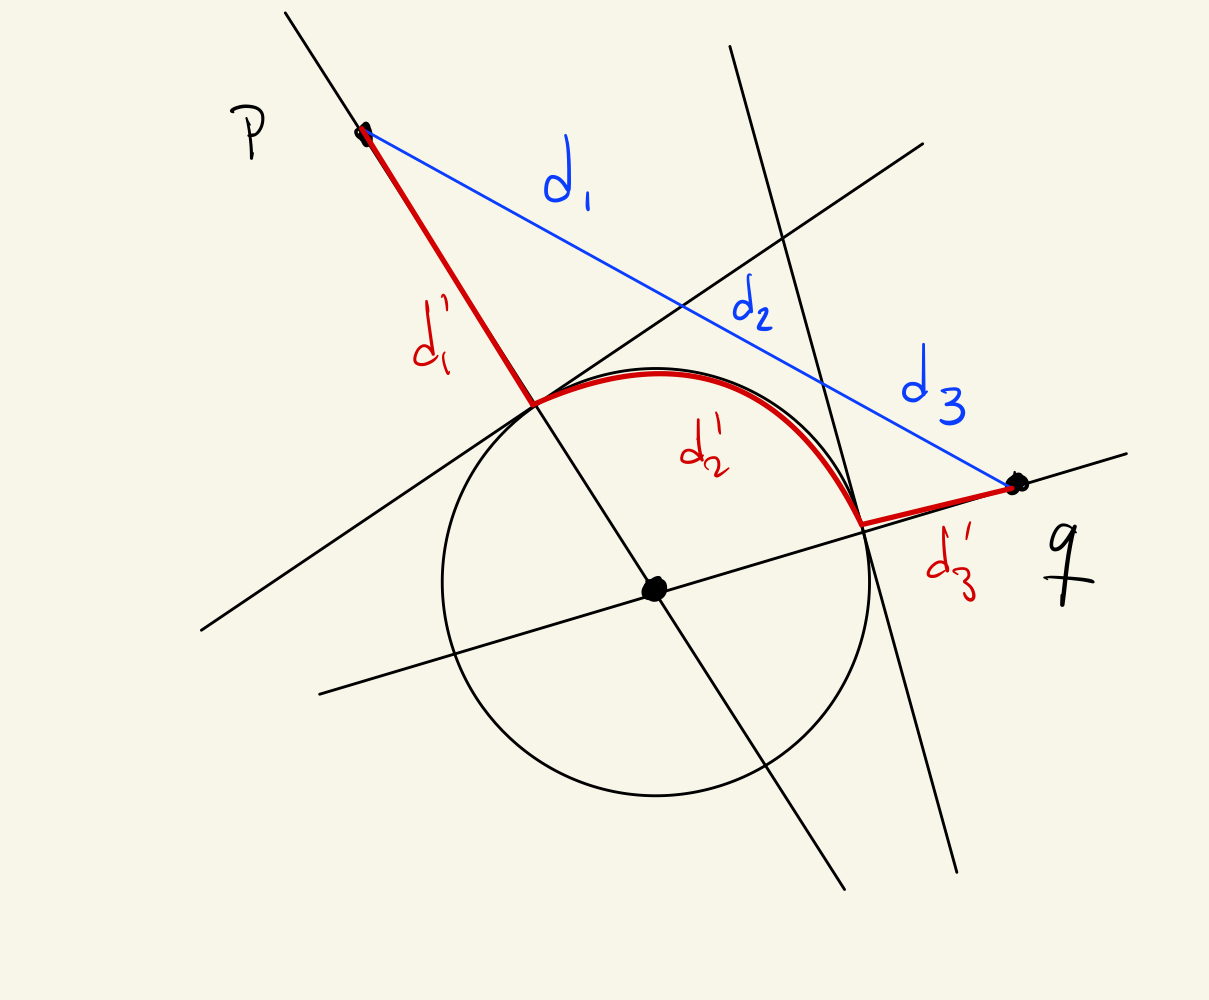
\includegraphics[width=0.6\textwidth]{fig1}
	\caption{Intento de prova}
\end{figure}

	Acabou que essa afirmação é simplesmente a lei dos cosenos, já que a distância esférica entre \(\frac{p}{\|p\|}\) e \(\frac{q}{\|q\|}\) é exatamente o angulo entre \(p\) e \(q\) (poque essa distância é um segmento de círculo máximo!):
	\[\text{lei dos cosenos:} \qquad d(p,q)^2=\|p\|^2+\|q\|^2-2\|p\|\|q\| \cos \angle(p,q) \]

Em fim, \(\tilde{A}\) é uma isometria porque \(d_{\mathbb{R}^{n+1}}(p,q)=d_{\mathbb{R}^{n+1}}(\tilde{A}p,\tilde{A}q)\) pelo argumento anterior. 
\end{enumerate}
\end{proof}

\begin{thing4}{Exercício 12}\label{exer:12}\leavevmode
Seja \((G,g)\) um grupo de Lie munido de uma métrica bi-invatiante e \(\nabla\) sua conexão de Levi-Civita.
\begin{enumerate}[label=(\alph*)]
\item Mostre que
	\[\nabla_uv=\frac{1}{2}[u,v],\]
	para cada \(u,v \in \mathfrak{g} \subset \mathfrak{X}(G)\).
\item Seja \(\overline{\nabla}\) uma conexão agim simétrica em \(G\). Mostre que \(\overline{\nabla}=\nabla\) se e somente se \(\overline{\nabla}_uu=0\) para todo \(u \in \mathfrak{g}\).
\end{enumerate}
\end{thing4}


\begin{proof}[Solution]\leavevmode
\begin{enumerate}[label=(\alph*)]
\item Como \(\nabla\) é Levi-Civita, temos Koszul, i.e. \(\forall  u,v,w \in \mathfrak{g}\),
	\begin{align*}
	2\left<\nabla_uv,w\right>&=u\left<v,w\right>+v\left<u,w\right>-w\left<u,v\right>\\
				 & -\left<u,[v,w]\right>+\left<v,[w,u]\right>+\left<w,[u,v]\right>
	\end{align*}
	Como \(\left<\cdot,\cdot\right>\) é invariante à esquerda, é constante quando avaliamos em elementos de \(\mathfrak{g}\), e portanto os primeiros três termos se anulam. Então o exercício acaba quando mostramos que
	\[\left<v,[w,u]\right>=\left<u,[v,w]\right>=-\left<u,[w,v]\right>.\]
	Seguindo \cite{doc}, p. 45., a ideia é usar o fluxo \(\varphi:\mathbb{R} \times G\to G\) de \(w\) para expressar o colchete de Lie. Primeiro precisamos de

	\begin{claim}\leavevmode
	O fluxo \(\varphi\) de um campo invariante à esquerda \(w\) comuta com a traslação à esquerda, i.e.,
	\[\varphi_t(e)\circ L_h = L_h \circ \varphi_t(e)\qquad \forall t\in \mathbb{R} \forall h \in G.\]
	\end{claim}
	\begin{proof}[Prova da afirmação]\leavevmode
Derivamos de ambos lados. Por um lado,
\begin{align*}
\frac{d}{dt}\Big|_{t=0}\varphi_t(e) \circ L_h=\frac{d}{dt}\Big|_{t=0}\varphi_t(h)&=v_h\end{align*}
Por outro lado,
\[\frac{d}{dt}\Big|_{t=0}L_h \circ \varphi_t(e)=(L_h)_{*,\varphi_t(e)}\frac{d}{dt}\Big|_{t=0}\varphi_t(e)=(L_h)_{*,e}v_e=v_h.\]
Por unicidade das soluções de EDOs, acabou.
	\end{proof}
Então repare:
\[\varphi_t(h)=(\varphi_t\circ L_h)(e)=(L_h \circ \varphi_t)(e)=h\varphi_t(e)=R_{\varphi_t(e)}h,\]
ou seja, qualquer curva integral de \(w\) é simplesmente a curva integral que passa por \(e\) trasladada.

Agora lembre que o colchete de Lie pode ser expressado como
\[[w,v]_e=\frac{d}{dt}\Big|_{t=0}\Big(\varphi_{-t}\Big)_{*,\varphi_t(e)}v_{\varphi_t(e)}.\]
(Onde fixamos o parámetro \(-t\) e deixamos livre o outro para ver \(\varphi_{-t}\) como um difeomorfismo de \(G\).)

Juntando com a discussão anterior obtemos
\[[w,v]_e=\frac{d}{dt}\Big|_{t=0}\Big(R_{\varphi_{-t}(e)}\Big)_{*,\varphi_t(e)}v_{\varphi_t(e)}.\]
Agora repare: como a métrica é bi-invariante,
\begin{align*}
\left<u,v\right>&=\left<\Big(R_{\varphi_{-t}(e)}\Big)_{*,\varphi_t(e)}\Big(L_{\varphi_{t}(e)}\Big)_{*,e}u_{e},\Big(R_{\varphi_{-t}(e)}\Big)_{*,\varphi_t(e)}\Big(L_{\varphi_{t}(e)}\Big)_{*,e}v_{e}\right>\\
&=\left<\Big(R_{\varphi_{-t}(e)}\Big)_{*,\varphi_t(e)}u_{\varphi_t(e)},\Big(R_{\varphi_{-t}(e)}\Big)_{*,\varphi_t(e)}v_{\varphi_t(e)}\right>
\end{align*}
Agora derivemos como funções de \(t\) (dentro de \(T_eG\), i.e. não precisamos derivada covariante), e avaliemos em  \(t=0\). (Note que quando avaliamos em  \(t=0\) o factor que não derivamos não muda---estamos trasladando à direita e à esquerda por \(\varphi_0(e)\)!) Obtemos:
\begin{align*}
0&=\frac{d}{dt}\Big|_{t=0}\left<\Big(R_{\varphi_{-t}(e)}\Big)_{*,\varphi_t(e)}u_{\varphi_t(e)},\Big(R_{\varphi_{-t}(e)}\Big)_{*,\varphi_t(e)}v_{\varphi_t(e)}\right>\\
 &=\left<\frac{d}{dt}\Big|_{t=0}\Big(R_{\varphi_{-t}(e)}\Big)_{*,\varphi_t(e)}u_{\varphi_t(e)},\left[\Big(R_{\varphi_{-t}(e)}\Big)_{*,\varphi_t(e)}v_{\varphi_t(e)}\right]_{t=0}\right>\\
&+\left<\left[\Big(R_{\varphi_{-t}(e)}\Big)_{*,\varphi_t(e)}u_{\varphi_t(e)}\right]_{t=0},\frac{d}{dt}\Big|_{t=0}\Big(R_{\varphi_{-t}(e)}\Big)_{*,\varphi_t(e)}v_{\varphi_t(e)}\right>\\
&=\left<[w,u]_e,v_e\right>+\left<u_e,[w,v]_e\right>.
\end{align*}
\end{enumerate}

\item Pelo inciso (a), é claro que se  \(\overline{\nabla}=\nabla\), \(\overline{\nabla}_u u=0\). Para a implicação contrária, vejamos que
	\[\overline{\nabla}_uv=\frac{1}{2}[u,v],\qquad u,v \in \mathfrak{g}\]
	que é conveniente porque sabemos que isso é igual a \(\nabla_uv\) pelo inciso (a). É só fazer:
	\[0=\overline{\nabla}_{u+v}u+v=\cancelto{0}{\overline{\nabla}_u u}+\overline{\nabla}_uv+\overline{\nabla}_vu+\cancelto{0}{\overline{\nabla}_vv}\]
Lembre que \(\overline{\nabla}\) é simétrica, i.e. \(\overline{\nabla}_uv-\overline{\nabla}_vu=[u,v]\). Somando com a equação anterior:
\begin{align*}
	\overline{\nabla}_uv-\overline{\nabla}_vu+\overline{\nabla}_uv+\overline{\nabla}_vu=[u,v]
\end{align*}
como queríamos. Para concluir é só ver que \(\nabla\) e \(\overline{\nabla}\) também coincidem em campos vetoriais que não são invariantes à esquerda. Então pegue uma base \(\{u_i\}\subset \mathfrak{g}\) e dois campos \(X=X^iu_i\),\(Y=Y^ju_j\) quaisquer. Então:
\begin{align*}
\overline{\nabla}_XY&=\overline{\nabla}_{X^iu_i}Y^ju_j=X^iu_iY_ju_j+Y^j\overline{\nabla}_{u_i}u_j=X^iu_iY_ju_j+Y^j\nabla_{u_i}u_j=\nabla_XY.
\end{align*}
\begin{question}\leavevmode
Tem algum argumento super simples para argumentar essa última parte sem pegar uma base de \(\mathfrak{g}\)?
\end{question}
\end{proof}

\begin{thing4}{Exercício 13}[Exercício 3, Cap. III, \cite{doc}]\label{exer:13}\leavevmode
Sejam \(G\) um grupo de Lie,  \(\mathfrak{g}\) sua álgebra de Lie, e \(X \in \mathfrak{g}\). As trajetórias de \(X\) determinam uma aplicação \(\varphi:(-\varepsilon,\varepsilon)\to G\) com \(\varphi(0)=e\), \(\varphi'(t)=X(\varphi(t))\).
\begin{enumerate}[label=(\alph*)]
\item Prove que \(\varphi(t)\) está definida para todo \(t \in \mathbb{R}\) e que \(\varphi(t+s)=\varphi(t)\cdot\varphi(s)\), (\(\varphi:\mathbb{R} \to G\) é então chamado um \textit{\textbf{subgrupo a 1-parâmetro de \(G\)}}.
\item Prove que se \(G\) tem uma métrica bi-invariante \(\left<\cdot,\cdot\right>\) então as geodésicas de \(G\) que partem de \(e\) são os subgrupos a 1-parâmetro de \(G\).
\end{enumerate}
\end{thing4}

\begin{proof}[Solution]\leavevmode
\begin{enumerate}[label=(\alph*)]
\item Lembre que no exercício anterior mostramos que
	\[\varphi_t(h)=R_{\varphi_t(e)}(h)=h\cdot \varphi_t(e),\qquad \forall t \in (-\varepsilon,\varepsilon),\;\forall h \in G.\]
	Fixe um \(t_0 \in (-\varepsilon,\varepsilon)\) e pegue \(h=\varphi_{t_0}(e)^{-1}\). Obtemos que
	\[\varphi_t(\varphi_{t_0}(e)^{-1})=\varphi_{t_0}(e)^{-1}\varphi_t(e).\]
Ou seja,  \(\varphi_{t_0}(e)^{-1}\varphi_t(e)\) é uma curva integral de \(X\) que passa por \(e\) no tempo \(t=t_0\). Como também \(\varphi_{t-t_0}(e)\) é uma curva integral de \(X\) que passa por \(e\) no tempo \(t=t_0\), por unicidade de EDOs obtemos
\begin{equation}\label{eq:2}
\varphi_{t_0}(e)^{-1}\varphi_t(e)=\varphi_{t-t_0}(e)
\end{equation}
Avaliando o lado esquerdo em \(t'=t-t_0\), do lado direito chegamos até \(\varphi_{t-2t_0}(e)\). Repetindo esse processo cobrimos todo \(\mathbb{R}\).

Para confirmar a segunda propriedade avaliamos \cref{eq:2} em \(t=0\) para obter \(\varphi_{t_0}(e)^{-1}=\varphi_{-t_0}(e)\). Para concluir pegue  \(t,s \in \mathbb{R}\) quaisquer e escreva:
\[\varphi_{t+s}(e)=\varphi_{t-(-s)}(e)=\varphi_{-s}^{-1}\varphi_t(e)=\varphi_s(e)\varphi_t(e).\]

\item Pegue \(X \in \mathfrak{g}\) e considere a curva integral que passa por \(e\), \(\varphi\). Pelo exercício anterior,
\[0=\nabla_X X=\nabla_{\varphi_*\frac{d}{dt}}X=\nabla_{\frac{d}{dt}}^\varphi X \circ \varphi=\nabla_{\varphi'}\varphi'\]
Então as curvas integrais de \(X\) que passam por \(e\) são geodésicas. Como isso é para qualquer vetor em \(\mathfrak{g}\), por unicidade das soluções a EDOs, acabou.
\end{enumerate}
\end{proof}

\clearpage
\begin{thing4}{Exercício 14}\label{exer:14}\leavevmode
Dada uma variedade Riemanniana \((M^n,g)\) denotamos por \(d_g\) a distância induzida por \(g\).
\begin{enumerate}[label=(\alph*)]
\item Sejam \(g,h\) duas métricas Riemannianas em \(M^n\). Mostre que se \(d_g=d_h\) então \(g=h\).
\item Seja \((M,g)\) uma variedade Riemanniana e \(F:M \to M\) um difeomorfismo. Mostre que \(F\) é uma isometria se e somente se \(d_g(F(\cdot),F(\cdot))=d_g(\cdot,\cdot)\).
\end{enumerate}
\end{thing4}

\begin{proof}\leavevmode
\begin{enumerate}[label=(\alph*)]
\item  Prova por contrapositiva.
	\begin{claim}\leavevmode
	Se \(g \neq h\), existem um aberto \(U\subset M\) e um marco \(\{E_i\}\subset \mathfrak{X}(U)\) tais que
	\[g(E_{i_0},E_{i_0}) \neq  h(E_{i_0},E_{i_0})\qquad \text{para algum } i_0\in \{1,\ldots,n\}.\]
	\end{claim}
	\begin{proof}[Prova da afirmação.]\leavevmode
	Se \(g(E_i,E_i)=h(E_i,E_i)\) para todo marco em todo aberto de \(M\), é claro que \[g(X,Y)=g(X^iE_i,Y^jE_j)=X^iY^jg(E_i,E_j)=h(X,Y)\]
para quaisquer \(X,Y \in \mathfrak{X}(M)\).
	\end{proof}
	Então pegue um marco \(\{E_i\} \in \mathfrak{X}(U)\) tal que \(g(E_{i_0},E_{i_0})\neq h(E_{i_0},E_{i_0})\) em \(U\). Sendo a diferença dessas quantidades uma função distinta da constante zero, podemos supô-la estritamente positiva dentro de \(U\). Pegue \(p \in U\) e uma vizinhança geodésica contendo \(p\), que renomeamos \(U\) por simplicidade. Dentro de uma vizinhança geodésica, a distância de \(p\) aos outros pontos dentro de \(U\) está realizada por geodésicas, então podemos pegar \(q \in U\) e \(\gamma\) geodésica ligando \(p\) e \(q\).

	Considere uma extensão de \(\gamma'\in \mathfrak{X}_\gamma\) dentro de \(U\), digamos \(G=G^iE_i\). Então:
	\begin{align*}
	d_g(p,q)&=\int_a^b g(G^iE_i,G^iE_i) \circ \gamma dt=\int_a^b (G^i \circ \gamma)^2g(E_i,E_i) \circ \gamma dt\\&\neq \int_a^b(G^i \circ \gamma)^2 h(E_i,E_i)\circ \gamma dt = d_h(p,q).
	\end{align*}

\item Primeiro suponha que \(F^*d_g=d_g\). Para mostrar que \(F\) é uma isometria usamos o inciso anterior: consideramos as métricas \(g\) e \(F^*g\) em \(M\). Basta mostrar que \(d_g=d_{F^*g}\). Por um tempo pensei que era para usar um câmbio de variáveis, mas acabei pensando assim: Pegue uma curva \(\gamma\) ligando \(p\) e \(q\). Note que
	\[\underbrace{\int_a^bF^* g(\gamma'(t),\gamma'(t))dt}_{\ell(\text{curva de \(p\) a \(q\)} )}=\underbrace{\int_a^bg(F_{*,\gamma(t)}\gamma'(t),F_{*,\gamma(t)}\gamma'(t))dt}_{\ell(\text{curva de \(F(p)\) a \(F(q)\)} )}\]
Ou seja, do lado esquerdo estamos medindo o comprimento (respeito à métrica \(F^*g\)) de uma curva ligando \(p\) a \(q\), enquanto que do lado direito estamos medindo o comprimento (respeito à métrica \(g\)) da curva \(F\circ \gamma\), que liga \(F(p)\) a \(F(q)\).

Pegando o ínfimo de ambas quantidades, concluímos que a distância \(d_{F^*g}\) coincide com a distância \(F^*d_g\), que por hipótese é igual a \(d_g\). A implicação contrária também fica clara: supondo que \(F^*g=g\), levando em conta a igualdade das integrais acima e pegando o ínfimo, concluímos que \(F^*d_g=d_g\).
\end{enumerate}
\end{proof}

\begin{thing4}{Exercício 15}\label{exer:15}\leavevmode
Suponha que \((M^n,g)\) é uma variedade Riemanniana conexa.
\begin{enumerate}[label=(\alph*)]
\item \((M,g)\) simétrica \(\implies\) \((M,g)\) homogênea.
\item \((M,g)\) 2-homogênea \(\implies\) \((M,g)\) isotrópica.
\end{enumerate}
\end{thing4}

\begin{proof}[Solution]\leavevmode
\begin{enumerate}[label=(\alph*)]
	\item \textbf{Ideia.} Pegamos dois pontos \(q, q' \in M\). Para usar que \(M\) é simétrica buscamos o ``ponto meio". Esse deve ser \(p\in M\) que esteja no meio do caminho de uma curva minimizante \(\gamma\) ligando \(q\) e \(q'\). Daí, pegamos \(F \in \operatorname{Iso}_p:=\{\text{ isometrias de \(M\) que fixam \(p\)}\}\) com a propriedade de que \(d_pF=-\operatorname{Id}\). Daí devemos provar que \(F\) preserva \(\gamma\) e não fixa \(q\). Daí, só existem dois pontos em \(\gamma\) que guardam a mesma distância com \(p\): \(q\) e \(q'\). Como  \(F(q)\neq  q\) também guarda essa distância, concluímos que \(F(q)=q'\).

Infelizmente fui incapaz de levar minha ideia até uma prova sem ajuda externa. Primeiramente me pareceu improvável a possibilidade de construir a geodésica minimizante (pode não existir para variedades não completas; mostrar que a propriedade de simetria implica a existência de curvas minimizantes parecia muito forte).

\begin{conjecture}
	 Para quaisquer \(q,q' \in M\) existe uma curva minimizante \(\gamma\) ligando \(q\) e \(q'\).
\end{conjecture}
	Supondo que existe \(\gamma\), podemos pegar \(F \in \operatorname{Iso}_p\) tal que \(d_pF=-\operatorname{Id}\) onde \(p\) é ponto meio sobre \(\gamma\) respeito \(q\) e \(q'\).

	Tentei mostrar que \(F\) preserva \(\gamma\) perto de \(p\) usando um marco geodésico, onde a geodésicas são curvas integrais de linhas, mas depois descobri que minha prova estava errada (pois \(dF\) só age como \(-\operatorname{Id}\) em \(p\)):
	\begin{thing8}{Afirmação}\leavevmode
	Perto de \(p\), \(F(\gamma(t)) \in \operatorname{img} \gamma\).
	\end{thing8}
	\begin{proof}[Prova da afirmação]\leavevmode
	Pegue coordenadas geodésicas centradas em \(p\), de modo que as curvas minimizantes como \(\gamma\) são imagens de retas em \(T_pM\) baixo a exponencial. Agora derivamos: \(F \circ \gamma\):
	\[\frac{d}{dt}\Big|_{t}F \circ \gamma=F_{*,\gamma(t)}\gamma'(t)=-\gamma'(t).\]
	Portanto, a derivada da curva \(F \circ \gamma\) coincide com a derivada de \(\gamma\). Por unicidade de soluções de EDOs, concluímos que \(F \circ \gamma(t) \in \operatorname{img} \gamma\) dentro desta bola geodésica.
	\end{proof}
Depois desse ponto comecei a buscar ajuda em livros, internet e ChatGPT. Rapidamente reparei que minhas ideias eram boas, e consegui:
	\begin{proof}[Prova da afirmação reforçada]\leavevmode
	Pegue coordenadas geodésicas centradas em \(p\), de modo que as curvas minimizantes como \(\gamma\) são imagens de retas em \(T_pM\) baixo a exponencial. Agora derivamos: \(F \circ \gamma\) em \(t=0\) (supondo que \(\gamma(0)=p\)):
	\[\frac{d}{dt}\Big|_{t=0}F \circ \gamma=F_{*,p}\gamma'(0)=-\gamma'(0).\]
	Portanto, a derivada da curva \((F \circ \gamma)(t)\) coincide com a derivada de \(\gamma(-t)\). Por unicidade de soluções de EDOs, concluímos que \(F \circ \gamma(t) \in \operatorname{img} \gamma\) dentro desta bola geodésica.
	\end{proof}
Seguindo com esse raciocínio, \(F \circ \gamma\) é uma curva definida em todo o domínio de \(\gamma\), e portanto deve coincidir com \(\gamma(-t)\) ao longo desse domínio. Ou seja, \(F \circ \gamma\) é \(\gamma\) percorrida em sentido oposto. Isso significa, por definição de \(p\) como ponto meio, e desde que supomos que \(\gamma(0)=p\), que, se \(\gamma(t_0)=q\), necessariamente \(q'=\gamma(-t_0)=(F \circ \gamma)(t_0)=F(q)\), como queríamos. (Note que meu desejo inicial de mostrar que \(F(q)\neq q'\) não foi necessário.)

Então tudo fica resolvido se mostramos a conjetura. O motivo inicial para conjeturar isso foi notar que \(\mathbb{R}^2\setminus\{0\}\), onde os pontos antípodas (entre outros) não podem ser ligados por curvas minimizantes, parece perder a propriedade de ser um espaço simétrico (que \(\mathbb{R}^{2}\) tem). Com efeito, a intuição mostra que \(\operatorname{Iso}(\mathbb{R}^2\setminus\{0\})=\mathsf{O}(2)\), de modo que o grupo de isotropia \(\operatorname{Iso}_p\) é trivial para todo ponto.

A inspiração final chega de \href{https://mathoverflow.net/questions/31009/action-of-the-group-of-isometries-on-a-manifold}{MathOverflow}: parece que, com efeito, toda variedade simétrica é completa:
\begin{quotation}
	``Consider a local geodesic and use the symmetry to flip it, effectively doubling the length of the geodesic, ad infinitum"
\end{quotation}
A ideia nos lembra do exercício que fizemos com grupos de Lie. Pegamos uma geodésica definida perto de \(p\). Pegamos \(q\neq p\) dentro da bola geodésica centrada em \(p\). Agora considere \(F \in \operatorname{Iso}_q\) tal que \(F_q = =\operatorname{Id}\). Sabemos que \(\gamma\) está definida entre \(p\) e \(q\), e, pela afirmação mostrada acima, compondo com \(F\) obtemos \(\gamma\) reparametrizada em sentido oposto. Isso permite chegar a um ponto sobre a curva original que fica à mesma distância de \(q\) que \(p\), só que no sentido oposto. Repetindo esse processo, vemos que a geodésica pode ser estendida infinitamente.

De fato, isso parece mostrar a conjetura via teorema de Hopf-Rinow, por exemplo em \cite{ler}, Lemma 6.18 e Coro. 6.20. Tem uma prova sem usar esse teorema?

\item Queremos ver que \(\forall p \in M\) e \(\forall v,w \in T^1_pM\) existe \(F \in \operatorname{Iso}_p(M)\) tal que \(F_{*,p}v=w\). Para usar a propriedade de ser 2-homogênea, defina  \(p_1:=q_1:=p\), e \(p_2:=\operatorname{exp}_p(v)\), \(q_2:=\operatorname{exp}_p(w)\). (Isto é, supondo por enquanto que \(\operatorname{exp}_p\) está definida em vetores de norma 1.) Então existe \(F \in \operatorname{Iso}(M)\) tal que \(F(p_1)=F(q_1)\), i.e. \(F \in \operatorname{Iso}_p(M)\), e tal que \(F(p_2)=F(q_2)\).

Para ver que \(F_{*,p}v=w\), note que \((F \circ \gamma_v)(1)=F(\gamma_v(1))=F(p_2)=q_2\). Então \(F \circ \gamma_v\) é uma curva ligando \(p\) e \(q\). Pelo exercício 14(b) dessa lista, como \(F\) é uma isometria, sabemos que preserva a distância, de modo a \(F \circ \gamma_v\) é minimizimante e portanto uma geodésica. Daí \(F \circ \gamma_v\) é uma reparametrização de \(\gamma_w\); mas como \(F\) é isometria, preserva a norma dos vetores velocidade e portanto as curvas coincidem. Isso significa que \(w=\gamma'_w(0)=(F \circ \gamma_v)'(0)=F_{*,p}\gamma_v'(0)=F_{*,p}v\).

Por último só note que se \(\operatorname{exp}_p\) não está definida em vetores de norma \(1\), podemos fazer a mesma construção em vetores que estejam dentro do domínio dela, obtendo uma função cuja diferencial envia um múltiplo pequeno de \(v\) em um múltiplo de igual proporção respeito a \(w\). A diferencial dessa função também envia \(v\) em \(w\), pois é uma isometria linear.
\end{enumerate}
\end{proof}

\clearpage
\begin{minipage}{\textwidth}
	\begin{minipage}{1\textwidth}
		{\small Prof. Luis Florit\hfill Daniel González Casanova Azuela}
		
		{\small Monitor. Ivan Miranda\hfill\href{https://github.com/danimalabares/rg}{github.com/danimalabares/rg}}
	\end{minipage}
\end{minipage}\vspace{.2cm}\hrule

\vspace{10pt}
{\huge Lista 4}
\addcontentsline{toc}{section}{Lista 4}

\begin{thing4}{Exercício 1}[Cap. IV Exer. 1, \cite{doc}]\label{exer:1}\leavevmode
Seja \(G\) um grupo de Lie com uma métrica \(\left<\cdot,\cdot\right>\) bi-invariante. Seja \(X,Y,Z\in\mathfrak{X}(G) \) campos unitários e invariantes à esquerda em \(G\).
\begin{enumerate}[label=(\alph*)]
	\item Mostre que \(\nabla_XY=\frac{1}{2}[X,Y]\). (Feito na lista 3.)
	\item Conclua de (a) que \(R(X,Y)Z=\frac{1}{4}[[X,Y],Z]\).
	\item Prove que, se \(X\) e \(Y\) são ortonormais, a curvatura seccional \(K(\sigma)\) de \(G\) segundo o plano \(\sigma\) gerado por \(X\) e \(Y\) é dada por
		\[K(\sigma)=\frac{1}{4}\|[X,Y]\|^.\]
		Portanto, \textit{a curvatura seccional \(K(\sigma)\) de um grupo de Lie com métrica bi-invariante é não negativa e é zero se e só se \(\sigma\) é gerado por vetores \(X,Y\) tais que \([X,Y]=0\).} 
		
\end{enumerate}
\end{thing4}

\begin{proof}[Solution]\leavevmode
\begin{enumerate}[label=(\alph*)]
	\item[(b)] 
		\begin{align*}
			R(X,Y)Z&=\nabla_X\nabla_YZ-\nabla_y\nabla_XZ-\nabla_{[X,Y]}Z\\
			       &=\frac{1}{2}\nabla_X[Y,Z]-\frac{1}{2}\nabla_Y[X,Z]-\frac{1}{2}[[X,Y],Z]\\
			       &=\frac{1}{4}[X,[Y,Z]-\frac{1}{4}[Y,[X,Z]]-\frac{1}{2}[[X,Y],Z]\\
			       &=\frac{1}{4}\Big([X,[Y,Z]]+[Y,[Z,X]+[Z,[X,Y]]\Big)+\frac{1}{4}[Z,[X,Y]]\\
			\text{identidade de Jacobi} \qquad &=\frac{1}{4}[Z,[X,Y]]
		\end{align*}
		que é exatamente o que queríamos a menos de um signo que muda com a convenção de \cite{doc} para \(R\).

	\item[(c)]
		\begin{align*}
		K(X,Y)&=\frac{R(X,Y,Y,X)}{\left<X,X\right>\left<Y,Y\right>-\left<X,Y\right>^2}\\
	&=R(X,Y,Y,X)=\left<R(X,Y)Y,X\right>\qquad 	\text{\(X\),\(Y\) ortonormais}\\
	&=\frac{1}{4}\left<[[X,Y],Y],X\right>\qquad \qquad \qquad 	\text{inciso (b) (convenção \cite{doc})}\\
		\end{align*}
		Agora lembre que na lista 3 provei que
		\[\left<[w,u],v\right>=-\left<u,[w,v]\right>\qquad \forall u,v,w \in \mathfrak{g}\]
		Pegue \(u=[X,Y]\), \(v=X\) e \(w=Y\) para obter
	\begin{align*}
		\left<[Y,[X,Y]],X\right>&=-\left<[X,Y],[Y,X]\right>=\left<[X,Y],[X,Y]\right>
	\end{align*}
	a por outra parte
	\[\left<[Y,[X,Y]],X\right>=-\left<[[X,Y],Y],X\right>\]
Então parece de novo que tá errado por um signo mas resulta que a definição de \(K\) também é outra em \cite{doc}, então por antisimetria de \(R\) nas últimas duas entradas o signo vira e tudo tá certo.
\end{enumerate}

\end{proof}

\begin{thing4}{Exercício 2}\label{exer:2}\leavevmode
Seja \((M,g)\) uma variedade Riemanniana.
\begin{enumerate}[label=(\alph*)]
\item Se \((M,g)\) é homogênea, então \(M\) possui curvatura escalar constante.
\item  Se \((M,g)\) é 2-homogênea, então \(M\) é Einstein.
\item Se \((M,g)\) é 3-homogênea, então \(M\) possui curvatura seccional constante.
\end{enumerate}
\end{thing4}

\begin{proof}[Solução]\leavevmode
\begin{enumerate}[label=(\alph*)]
\item (Começarei com o inciso (b), pois foi o que consegui fazer melhor.)
\item \textbf{(Intento sem ajuda externa. Com pouco de pena mas da para mostrar, pode poular.)} Queremos ver que existe \(\lambda\in \mathbb{R}\) tal que \(\lambda\operatorname{Ric}=g\). Como tanto \(\operatorname{Ric}\) quanto \(g\) são tensores, basta mostrar o resultado numa base do espaço tangente a qualquer ponto. Usamos o exercício 15(b) da lista 3 para obter que \(M\) é isotrópica, i.e. \(\forall u,v \in T^1_pM\) existe \(f \in \operatorname{Iso}(M)\) tal que \(f_{*,p}u=v\).

	Para uma base ortonormal \(E_i\) de \(T_pM\) temos que
	\begin{align*}
	\operatorname{Ric}(E_i,E_j)&=\sum_{k}\left<R(E_k,E_i)E_j,E_k\right>\\
	&=\sum_{k}\left<R(E_i,E_k)E_k,E_j\right>\\
	&=\sum_{k}\left<R(E_i,E_k)E_k,f_{*}E_i\right>
	\end{align*}
onde existe \(f\in \operatorname{Iso}\)	tal que \(f_*E_i=E_j\) porque \(M\) é isotrópica. Daí (aqui começo a ter dúvida) usamos que \(f^*R=R\), ou seja
\[R(f_*E_i,f_*E_k)f_*E_k=R(E_i,E_k)E_k\]
isso é porque \(f\) é uma isometria e \(R\) depende da métrica e suas derivadas. Então a equação acima vira
\begin{align*}\operatorname{Ric}(E_i,E_j)&=\sum_{k}\left<R(f_*E_i,f_*E_k)f_*E_k,f_*E_i\right>\\&=\sum_{k}\left<R(E_i,E_k)E_k,E_i\right>\\
&=\sum_{k}K(E_i,E_k)\end{align*}
que não faz sentido.

\textbf{(Solução depois de consultar o professor + ChatGPT.)} A observação central feita pelo professor é considerar o endomorfismo associado a \(\operatorname{Ric}\), que definimos como \(\widehat{\operatorname{Ric}}\) satisfazendo
\[\left<\widehat{\operatorname{Ric}}(v),w\right>=\operatorname{Ric}(v,w)\]
A observação central feita pelo ChatGPT é que para uma isometria \(f\) temos que
\[f^*\operatorname{Ric}=\operatorname{Ric} \implies f_*\circ\widehat{\operatorname{Ric}}=\widehat{\operatorname{Ric}}\circ f_*\]
De fato, para \(v,w \in T_pM\),
\begin{align*}
\left<\widehat{\operatorname{Ric}}(f_*v),w\right>&=\operatorname{Ric}(f_*v,w)=f^*\operatorname{Ric}(v,f_*^{-1}w)=\operatorname{Ric}(v,f_*^{-1}w)\\
&=\left<\widehat{\operatorname{Ric}}v,f_*^{-1}w\right>=\left<f_*\widehat{\operatorname{Ric}}v,w\right>
\end{align*}
Agora mostramos que \(\widehat{\operatorname{Ric}}=\lambda \operatorname{Id}\). Então como \(\operatorname{Ric}\) é simétrico, \(\widehat{\operatorname{Ric}}\) é diagonalizável e da para calcular o seus eigenvalores. Vamos ver todos eles coincidem. Pegue \(v,w\) eigenvetores de norma 1. Como \(M\) é 2-homogênea, sabemos que é isotrópica e existe \(f\) isometria tal que \(f_*w=v\).
\begin{align*}
\lambda_v v=\widehat{\operatorname{Ric}}v=\widehat{\operatorname{Ric}}(f_*w)=f_*\widehat{\operatorname{Ric}}(w)=f_* \lambda_w w=\lambda_w f_* w=\lambda_w v
\end{align*}
então \(\lambda_v=\lambda_w\) como queríamos. E isso mostra que em cada ponto,
\[\operatorname{Ric}(v,w)=\left<\widehat{\operatorname{Ric}}v,w\right>=\left<\lambda v,w\right>=\lambda\left<v,w\right>\]
ou seja, \(\lambda\) é na verdade uma função em \(M\). Para ver que ela é constante, note que a condição de 2-homogeneidade implica homogeneidade, então \(\operatorname{Iso}\) age transitivamente em \(M\). Ou seja para \(p\neq q\) pontos em \(M\) existe \(f\) isometria tal que \(f(p)=q\). Como essa isometria preserva tanto o tensor de Ricci quanto a métrica, obtemos que
\begin{align*}\lambda(q)g_q&=\operatorname{Ric}_q=\operatorname{Ric}_{f(p)}=(f^* \operatorname{Ric})_{p}=\operatorname{Ric}_p\\&=\lambda(p)g_p=\lambda(p) (f^* g)_p=\lambda(p)g_{f(p)}=\lambda(p)g_{q}.
\end{align*}

\item \textbf{(Sem ajuda externa nem muito tempo para aprofundar!)} Minha ideia é assim: para controlar a curvatura seccional a partir da 3-homogeneidade realizamos dois vetores arbitrários \(v,w \in T_pM\) como sendo as derivadas de duas curvas: uma ligando \(p\) a \(q\), e outra ligando \(p\) a \(q'\). Agora nos perguntamos como é a curvatura em outro ponto  \(\hat{p}\). Transportamos a terna \((p,q,q')\) com uma isometria a alguma terna \((\hat{p},\hat{q},\hat{q'})\). Essa segunda terna pode ser escolhida de maneira que as correspondentes derivadas sejam quaisquer outros vetores \(\hat{v}\) e \(\hat{w}\) tangentes a \(\hat{p}\). As curvaturas seccionais coincidem porque \(f\) é uma isometria.
\item[(a)] \textbf{(Sem ajuda externa nem muito tempo para aprofundar!)} Uma isometria preserva a curvatura escalar. Como para todo \(p \neq q\) em \(M\) existe isometria \(f\) tal que \(f(p)=q\), obtemos que
	\[\operatorname{Scal}(q)=\operatorname{Scal}(f(p))=(f^*\operatorname{Scal})(p)=\operatorname{Scal}(p).\]
\end{enumerate}
\end{proof}

\begin{thing4}{Exercício 5}[Exer. 4, Cap IV, \cite{doc}]\label{exer:5}\leavevmode
Seja \(M\) uma variedade Riemanniana com a seguinte propriedade: dados dois pontos quaisquer \(p,q \in M\), o transporte paralelo de \(p\) a \(q\) não depende da curva que liga \(p\) a \(q\). Prove que a curvatura de \(M\) é identicamente nula, isto é, para todo \(X,Y,Z \in \mathfrak{X}(M)\), \(R(X,Y)Z=0\).
\end{thing4}

\begin{proof}\leavevmode
Parece que a sugestão é a prova quase por completo. Começarei explicando os pontos que achei que era necessário destrinchar para chegar a uma prova formal, e depois escrevo o argumento completo (que é basicamente uma copia da sugestão).

Concluir o exercício só depende de duas coisas:
\begin{enumerate}
	\item \textbf{(Mostrar que \(f\) sempre existe.)} A prova formalmente começa pegando três vetores \(X(p),Y(p),Z(p)\) no espaço tangente a um ponto arbitrário \(p \in M\). Primeiro devemos mostrar que existe \(f:U \to M\) tal que \(\partial_s|_{(0,1)} = X(p)\), \(\partial_t|_{(0,1)}=Y(p)\), e que \(f(s,0)=f(0,0)\).

	Primeiro usamos a exponencial \(\operatorname{exp}_p\) de \(M\) para definir a superfície como a imagem do subespaço vetorial gerado por \(X(p)\) e \(Y(p)\). A exponencial fica determinada numa bola aberta \(B_\varepsilon(0)\subset T_pM\). Note \(X(p)\) e \(Y(p)\) podem não estar contidos em \(B_\varepsilon(0)\), mas podemos consertar isso redefinindo a exponencial avaliando as geodésicas em valores menores do que 1. Agora compomos com uma função suave \(g:U \to B_{\varepsilon}(0)\) tal que
\begin{itemize}
\item \(g(0,1)=(0,0)\), de modo que  \(p=(\widetilde{\operatorname{exp}}_p^{-1} \circ g)(0,1)\).
\item \(g(s,0)=g(0,0)\).
\item \(g_{*,(0,1)}e_1=X(p)\).
\item \(g_{*,(0,1)}e_2=Y(p)\).
\end{itemize}
Então \(f=\widetilde{\operatorname{exp}}^{-1}_p\circ g\). \textbf{(Faltou: por que sempre existe \(g\)?)}

\item \textbf{(Mostrar que \(Z(p)\) pode ser atingido como o transporte paralelo de \(V(0,0)\).)} Isso é simples: definimos \(V(0,0)\) como o transporte paralelo de \(Z(p)\) a \(f(0,0)\). Por unicidade do transporte paralelo, acabou.
\end{enumerate}

Agora escrevo a prova completa. Como \(R\) é um tensor, basta mostrar o resultado num ponto só. \(R\) depende de três vetores. 

Para escolher os primeiros dois consideramos a superfície dada como a imagem do mapa \(f:U \subset \mathbb{R}^2 \to M\) construído acima, cujo domínio \(U\) é um quadrado aberto contendo o quadrado unitário:
\[U:=\{(s,t)\in \mathbb{R}^2;-\varepsilon<t<1+\varepsilon,-\varepsilon<s<1+\varepsilon,\varepsilon>0\}\]
Definimos um campo vetorial pegando um vetor arbitrário \(V_0 \in T_{f(0,0)}M\) e transportamos paralelamente ao longo das curvas verticais \(t \mapsto  (s,t)\). Isso significa que \(\nabla_{\partial_t}V=0\), e concluimos que
	\[\nabla_{\partial_s}\nabla_{\partial_t}=0=\nabla_{\partial_t}\nabla_{\partial_s}V+R(\partial_t,\partial_s)V\]
onde todos os campos são seções ao longo de \(f\) e \(R\) realmente é \(R_{\nabla^f}=f^*R\).

Agora notamos que \(V(1,0)\) deve ser, além do transporte paralelo de \(V(0,0)\) ao longo de \(t \mapsto (0,t)\), o transporte paralelo de \(V(0,0)\) ao longo de \(t \mapsto (s,t)\) seguido de \(s \mapsto (s,1)\) para  qualquer \(s\). Concluímos que \(\nabla_{\partial_s}V(s,1)=0\). Isso significa que \(R_{f(0,1)}=0\).

\begin{figure}[H]
	\centering
	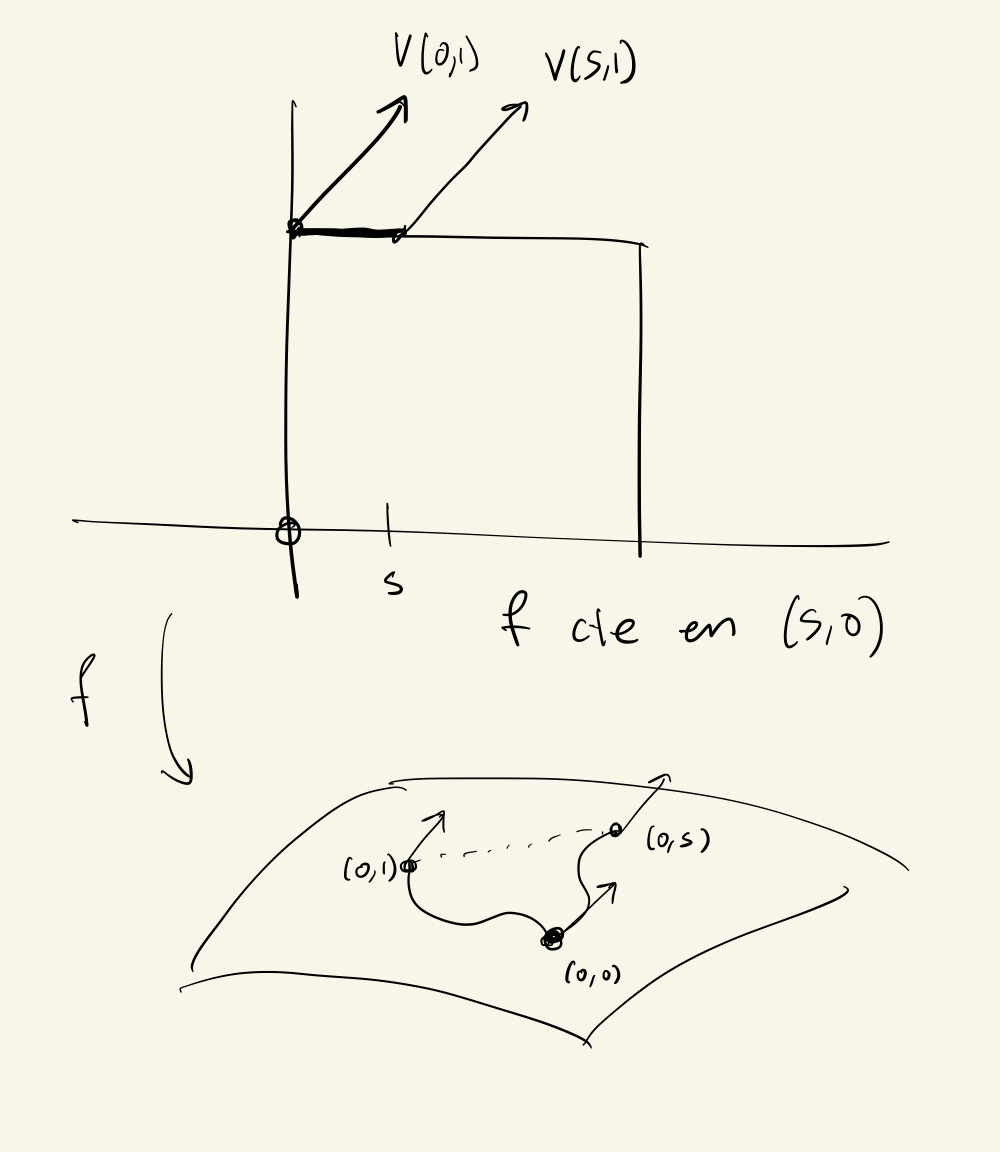
\includegraphics[width=0.5\textwidth]{fig4}
\end{figure}
\end{proof}

\clearpage

\addcontentsline{toc}{subsection}{Campos de Killing}
\section*{Campos de Killing}

\begin{thing4}{Exercício 11}[Exer. 5, Cap. III, \cite{doc}]\label{exer:11}\leavevmode
Sejam \(M\) uma variedade Riemanniana e \(X \in \mathfrak{X}(M)\). Seja \(p \in M\) e sejam \(U \subset M\) uma vizinhança de \(p\), e \(\varphi:(-\varepsilon,\varepsilon-)\times U \to M\) uma aplicação diferenciável tais que para todo \(q \in U\) a curva \(t \mapsto  \varphi(t,q)\) é a trajetória de \(X\) passando por \(q\) em \(t=0\). \(X\) é chamado um \textit{\textbf{campo de Killing}} (ou uma \textit{\textbf{isometria infinitesimal}}) se, para todo \(t_0\in (-\varepsilon,\varepsilon)\) a aplicação \(\varphi(t_0):U \subset M \to M\) é uma isometria. Prove que
\begin{enumerate}[label=(\alph*)]
\item Um campo linear em \(\mathbb{R}^n\), definido por uma matriz \(A\) é um campo de Killing se e só se \(A\) é anti-simétrica.
\item Seja \(X\) um campo de Killing em \(M\), \(p \in M\) e \(U\) uma vizinhança normal de \(p\) em \(M\). Admita que \(p\) é o único ponto de \(U\) que satisfaz \(X(p)=0\). Então, em \(U\), \(X\) é tangente às esferas geodésicas centradas em \(p\).
\item  Sejam \(X\) um campo diferenciável de vetores em \(M\) e \(f:M \to N\) uma isometria. Seja \(Y\) o campo de vetores em \(N\) definido por \(Y(f(p))=df_p(X(p))\), \(p \in M\). Então \(Y\) é um campo de Killing se e somente se \(X\) também o for.
\item \(X\) é de Killing \(\iff\) \(\left<\nabla_YX,Z\right>+\left<\nabla_ZX,Y\right>=0\) para todo \(Y,Z \in \mathfrak{X}(M)\) (a equaçao acima é chamada \textit{\textbf{equação de Killing}}).
\item Seja \(X\) um campo de Killing em \(M\) com \(X(q)\neq 0\), \(q \in M\). Então existe um sistema de coordenadas \((x_1,\ldots,x_n)\) em uma vizinhança de \(q\), de modo que os coeficientes \(g_{ij}\) da métrica neste sistema de coordenadas não dependem de \(x_n\).
\end{enumerate}
\end{thing4}

\begin{proof}[Solução]\leavevmode
\begin{enumerate}[label=(\alph*)]
	\item[(d)] Seguimos a sugestão usando \cite{les}.

	\begin{remark}\leavevmode
	Note que \(X\) é de Killing \(\iff\) \(\mathcal{L}_Xg=0\). A ida da para escrever com a definição de derivada de Lie de campos tensoriales covariantes:
	\[(\mathcal{L}_Xg)_p(Y,Z)=\frac{d}{dt}\Big|_{t=0}g_{\varphi_t(p)}(\varphi^t_{*,p}Y_p,\varphi^t_{*,p}Z_p)=\frac{d}{dt}\Big|_{t=0}g_p(Y_p,Z_p)=0\]
onde escrevo o fluxo como \(\varphi_t\) ou \(\varphi^t\) a vontade para facilitar notação. A volta também é simples usando Thm 12.37 \cite{les}: \((\varphi_t^*g)_p=g_p \iff L_Xg=0\).
	\end{remark}
	Usando essa observação o inciso (d)  pode ser resolvido assim: \(X\) killing \(\iff\) \(L_Xg=0\). Desenrolamos essa definição usando Prop. 12.32(d) \cite{les}:
	\begin{align*}
		0=(L_Xg)(Y,Z)&=L_X(g(Y,Z))-g(L_XY,Z)-g(Y,L_XZ)\\
			     &=X\left<Y,Z\right>-\left<[X,Y],Z\right>-\left<Y,[X,Y]\right>
	\end{align*}
	Como \(\left<\cdot,\cdot\right>\) é simétrica,
	\begin{align*}
	X\left<Y,Z\right>&=\left<\nabla_XY,Z\right>-\left<\nabla_YX,Z\right>\\
	&+\left<\nabla_XZ,Y\right>-\left<\nabla_ZX,Y\right>
	\end{align*}
	Como \(\left<\cdot,\cdot\right>\) é métrica, acabou.

\item Noto que para todo \(p=(p^1,\ldots,p^n) \in \mathbb{R}^n\),
	\[\frac{d}{dt}\Big|_{t=0}\varphi(t,p)=X_p=A(p).\]
	Consegui escrever
	\[\frac{d}{dt}\Big|_{t=0}\varphi(t,p)^i=a_{ij}p^j\]
pensando nas funções coordenadas de \(\varphi(t,p)\). Porém, não vi que isso é um sistema de equações diferenciais! Divaguei um tempo sem chegar a nada. Consultando ChatGPT, da para escrever
\[\begin{cases}
	\dot \varphi(t,p)=A \varphi(t,p) \\
	\varphi(0,p)=p\qquad
\end{cases}\]
que tem solução
\[\varphi(t,p)=e^{tA}\varphi(0,p).\]
Isso faz sentido pelas propriedades da exponencial de matrizes, en particular o fato que que
\[\frac{d}{dt}e^{tA}=Ae^{tA}\qquad \text{\cite{hall}, Prop. 2.4} \]
que implica que efetivamente a função \(e^{tA}\varphi(0,t)\) é solução do sistema dado acima. (Explorei outras formas de resolver o sistema, mas achei essa explicação mais familiar.)

Então concluímos que o fluxo é um mapa linear (a exponencial de matrizes é uma matriz). Como além disso é uma isometria, segue que é um elemento de \(\mathsf{O}(n)\). Agora lembre que a exponencial de grupos de Lie, que coincide com a exponencial de matrizes nesse caso, é um mapa da álgebra de Lie ao grupo. Como \(\operatorname{exp}(tA)\in\mathsf{O}(n)\), concluímos que \(A \in \mathfrak{o}(n)\). Para concluir só devemos confirmar que \(\mathfrak{o}(n)\) consta das matrizes antisimetricas. Note que
\begin{align*}
0=\frac{d}{dt}\Big|_{t=0}\left<\operatorname{exp}(tA)x,\operatorname{exp}(tA)y\right>&=\left<Ax,y\right>+\left<x,Ay\right>
\end{align*}
onde \(\left<\cdot,\cdot\right>\) é o produto ponto euclidiano. De fato, podemos reescrever as parcelas como
\[\left<Ax,y\right>=(Ax)^{\mathbf{T}}y=x^{\mathbf{T}}A^{\mathbf{T}}y,\qquad \qquad \left<x,Ax\right>=x ^{\mathbf{T}}(Ay)\]
obtendo que
\[0=x ^{\mathbf{T}}(A^{\mathbf{T}}+A)y\]
ou seja, \(A^{\mathbf{T}}+A=0\). (Argumento do Misha; também era natural pegar uma curva em \(\mathsf{O}(n)\) e derivar.)
\item Note que \(\varphi_t\) é uma isometria de \(B_\varepsilon(p)\). Isso segue de que \(\varphi_t(p)=p\) para todo \(t\). Isso segue de que a curva constante \(p\) satisfaz a equação do fluxo \(0=X_p=\frac{d}{dt}\Big|_{t=0}\varphi_t(p)\) e a mesma condição inicial. Daí segue que, como \(\varphi\) preserva a métrica riemanniana e portanto a distância riemanniana, ele manda esferas geodésicas em esferas geodésicas. Segue que as derivadas do fluxo, i.e. vetores de \(X\) são tangentes às esferas geodésicas.
	
\item Parece que segue da ``Propriedade de naturalidade dos fluxos", uma proposição em \cite{les}. Vejamos se posso escrever o essencial: basta mostrar que o fluxo de  \(\tilde{X}:=f_*X\) é dado por \(f \circ \varphi\) onde \(\varphi\) é o fluxo de \(X\). Basta diferenciar \(f \circ \varphi\) e comprovar que sua derivada coincide com \(\tilde{X}\) em cada ponto. Por unicidade de EDOs, acabou. E sim: \((f \circ \varphi_p)'(0)\) é, por definição de vetores como velocidades de  curvas, \(f_*(\varphi_p'(0))=f_* X\).

	Seja \(\tilde{\varphi}\) o fluxo de \(\tilde{X}\). Para ver que \(\tilde{\varphi}_t\) é uma isometria para todo \(t\), note que para todo \(\tilde{p}=f(p)\in \tilde{M}\) temos que
	\[\tilde{\varphi}_t(\tilde{p})=\tilde{\varphi}_{\tilde{p}}(t)=(f \circ \varphi_{p})(t)=f(\varphi_t(p))\]
é isometria porque \(f\) e \(\varphi_t\) são isometrias. (A troca do subíndice no fluxo me serve para pensar o fluxo como curva ou como isometria.)

\item[(e)] Queremos mostrar que \(\frac{\partial }{\partial x^n}g_{ij}=0\) para todo \(i,j\) naquele sistema coordenado. A escolha natural é o sistema coordenado onde \(X=\partial_n\). Como \(X\) é Killing vemos que:
	\[0=L_{\partial_n}(g_{ij}dx^idx^j)=(\partial_ng_{ij})dx^idx^j+g_{ij}L_{\partial_n}dx^idx^j\]
de novo pelas propriedades da derivada de Lie para campos tensoriais em \cite{les}. Lembre que \(dx^i dx^j\) denota a simetrização de \(dx^i \otimes dx^j \in \Gamma(T^*M \otimes T^*M)\), que  é igual a \(\frac{1}{2}(dx^i \otimes dx^j+dx^j\otimes dx^i)\) (quase) por definição---é uma conta pequena com a definição de simetrização de tensores. Basta argumentar que a segunda parcela da equação anterior se anula. Então temos que
\begin{align*}2L_{\partial_n}(dx^i dx^j)&=(L_{\partial_n}dx^i)\otimes dx^i+ dx^i \otimes (L_{\partial_n}dx^j)\\&+(L_{\partial_n}dx^j) \otimes dx^i+dx^j \otimes (L_X dx^i)\end{align*}

Lembremos a definição da derivada de Lie de campos tensoriais:
\[L_{\partial_n}dx^i:=\frac{d}{dt}\Big|_{t=0}\varphi^*_t dx^i\]
onde para \(V \in \mathfrak{X}(M)\) o pullback de campos tensoriais é definido por 
\[(\varphi^*_tdx_i)_p:=(dx^i)_{\varphi(t,p)}(\varphi^t_{*,p}V_p)\]
Minha intuição é que o fluxo de \(\partial_n\) não modifica as coordenadas de \(V\) distintas de \(V^n\), mas talvez essa última sim. No caminho para comprovar isso descobri que de fato o pushforward é a identidade. Vamos calcular o fluxo de \(X=\partial_n\) (aqui usei ChatGPT):
\[x \circ \varphi_p(t)=\Big((x^1 \circ \varphi_p)(t),\ldots,(x^n \circ \varphi_p)(t)\Big):=(\varphi^1(t),\ldots,\varphi^n(t))\]
obtemos o sistema
\[\dot \varphi^i(t)\begin{cases}
	0\qquad & i\neq  n\\
	1\qquad & i=n
\end{cases}\]
que implica que
\[\varphi^i(t)=\begin{cases}
	x(p)\qquad & i\neq n\\
	x(p)+t\qquad i=n&
\end{cases}\]
dada a condição inicial \(x \circ\varphi(0)=x(p)\). Então aqui, para minha surpresa, acaba que, dado \(t\) fixo, a derivada do fluxo \(\varphi_t\) é a identidade. E sim, porque como difeomorfismo de  \(M\) vemos em coordenadas que trata-se do mapa
\[(x^1(p),\ldots,x^n(p))\longmapsto (x^1(p),\ldots,x^n(p)+t),\]
e quando derivamos, como \(t\) é fixo, obtemos a matrix identidade. Concluimos que \(\varphi^*_{t}V\) é constante respeito a \(t\), de modo que a derivada de Lie é zero. Note que o fato de que a derivada do fluxo é a identidade não significa que \(L_{\partial_n}\omega=0\) para outros campos tensoriais, pois embora o pushforward dos campos vetoriais não é modificado por \(\varphi\), outros campos tensoriais podem variar de ponto a ponto, de modo que o pullback não é constante.
\end{enumerate}
\end{proof}

\begin{thing4}{Exercício 14}[Exer. 12, Cap. VI, \cite{doc}, Singularidades de um campo de Killing]\label{exer:14}\leavevmode
Seja \(X\) um campo de Killing em uma variedade Riemanniana \(M\). Seja \(N=\{p \in M; X(p)=0\}\). Prove que
\begin{enumerate}[label=(\alph*)]
\item Se \(p \in N\), \(V \subset M\) é uma vizinhança normal de \(p\), e \(q \in N \cap V\), então o segmento de geodésica radial \(\gamma\) ligando \(p\) a \(q\) está contido em \(N\). Conclua que \(\gamma \cap V \subset N\).
\item Se \(p \in N\), existe uma vizinhança \(V \subset M\) de \(p\) tal que \(V \cap N\) é uma subvariedade de \(M\) (Isto implica que toda componente conexa de \(N\) é uma subvariedade de \(M\)).
\item A codimensão, como subvariedade de \(M\), de uma componente conexa \(N_k\) de \(N\) é par. Admita o seguinte fato: se uma esfera possui um campo diferenciável não nulo então sua dimensão é ímpar.
\end{enumerate}
\end{thing4}

\begin{proof}[Solução]\leavevmode
\begin{enumerate}[label=(\alph*)]
\item Suponha que existe um ponto \(\gamma(t_0)\) sobre \(\gamma\) onde \(X\) não é nulo.  Como \(X\) é de Killing, o fluxo preserva a distância, i.e. sabemos que para qualquer \(s\),
	\begin{align*}
	\varepsilon_1:=d(\gamma(t_0),p)&=d(\varphi_s(\gamma(t_0)),\varphi_s(p))=d(\varphi_s(\gamma(t_0)),p)
	\end{align*}
	de modo que \(\varphi_s(\gamma(t_0))\) está na esfera de raio \(\varepsilon_1\) centrada em \(p\). Porém, o mesmo acontece com \(q\), i.e. \(\varphi_s(\gamma(t_0))\) está na esfera de raio \(\varepsilon_2:=d(\gamma(t_0),q)\) centrada em \(q\). Essas duas esferas se intersectam tangencialmente em \(\gamma(t_0)\) pelo lema de Gauss, e portanto o ponto de interseção é único numa vizinhança dele. Isso significa que o fluxo é constante em \(\gamma(t_0)\) e portanto \(X(\gamma(t_0))=0\).

	\item \textbf{(Solução seguindo a sugestão.)} Devemos mostrar que para todo \(t \in \mathbb{R}\), a restrição da diferencial do fluxo \(\varphi^t_*\) a  \(Q:=\operatorname{span}(\operatorname{exp}_p^{-1}(q_1),\operatorname{exp}_p^{-1}(q_2))\) é a identidade. Isso resulta claro pelo exercício 3 da lista 3: como \(\varphi^t\) é uma isometria,
		\[\varphi^t \circ \operatorname{exp}_p=\varphi^t_* \circ \operatorname{exp}_p\]
Defina \(v_1=\operatorname{exp}^{-1}(q_1)\). Como \(q_1\) é um ponto fixo de \(\varphi_t\),
\begin{align*}\varphi^t(\operatorname{exp}_p(v_1))=\operatorname{exp}_p(v_1)
\end{align*}
Pela observação da lista 3, esse ponto também é
\begin{align*}
\operatorname{exp}_p(\varphi_*^t(v_1))=\operatorname{exp}_p(v_1)
\end{align*}
Então, como \(\operatorname{exp}_p\) é bijetiva,
\begin{align*}
\varphi_*^t(v_1)&=v_1
\end{align*}
Agora defina \(v_2=\operatorname{exp}^{-1}(q_2)\); o mesmo argumento funciona. E mesmo para qualquer \(v:=av_1+b v_2 \in \operatorname{span}(v_1,v_2)\). Segue que em qualquer ponto de \(N_2:=\operatorname{exp}\Big(\operatorname{span}(v_1,v_2)\Big)\) o fluxo tem derivada zero e portanto \(X\) se anula. O procedimento funciona igual em dimensões maiores.

\item \textbf{(Seguindo a sugestão.)} A ideia é construir um campo vetorial diferenciável não nulo em alguma esfera contida no espaço \(N^\perp\). Isso significa que a dimensão da esfera é ímpar, e portanto a dimensão de \(N^\perp\) deve ser par.

	A prova acaba sendo bem parecida ao argumento que eu dei para o inciso (a), onde mostrei que os vetores não nulos de um campo de Killing num ponto \(q\) perto de \(p \in N\) devem ser tangentes a alguma esfera centrada em \(p\). Além disso, o campo  \(X\) não pode se anular em pontos dessa esfera \textbf{(por que? :( )}. Portanto, a restrição de \(X\) a essa esfera é um campo que não se anula.

	Além disso, como \(\varphi^t\) é uma isometria, notamos que preserva o espaço normal \(E_p:= (T_pN)^\perp\). Isso implica \textbf{(por que?)} que todo vetor de um campo de Killing que não seja zero deve ser tangente a \(N^\perp\).
\end{enumerate}
\end{proof}

\begin{thing4}{Exercício 15}[Fórmula de Bochner para campos de Killing]\label{exer:15}\leavevmode
	Seja \((M,g)\) uma variedade Riemanniana, \(X \in \operatorname{Kil}(M,g)\) e \(f:=\frac{1}{2}|X|^2\in C^\infty(M)\). Mostre que
	\[\Delta f= |\nabla X|^2-\operatorname{Ric}(X,X)\]
onde \(|\nabla X|(p)\) denota a norma do operador \(T_pM \ni v \mapsto \nabla_vX \in T_p M\).	
\end{thing4}

\textit{Ideias.} \hspace{.5em} Certamente não consegui resolver esse exercício. Aqui vão algumas ideias e perguntas:
\begin{enumerate}
	\item[0.] A ``norma do operador \(T_pM \ni v \mapsto \nabla_vX \in T_p M\)" é
		\[|X|:=\operatorname{sup}_{|v|=1}\nabla_vX\qquad ?\]
		
	\item Tentei fazer algumas contas:
		\begin{align*}
\Delta f&=\Delta \left(\frac{1}{2}|X|^2\right) =\frac{1}{2}\nabla \left<X,X\right>
\end{align*}
Onde, para \(Y \in \mathfrak{X}(M)\), sabemos que
\begin{align*}
\left<\nabla \left<X,X\right>,Y\right>&=Y\left<X,X\right>=2\left<\nabla_YX,X\right>.
\end{align*}
Agora pegue um marco ortonormal \(E_i\), de modo que
\begin{align*}
\Delta f&=\sum_{i} \left<\nabla_{E_i}\nabla f,E_i\right>
\end{align*}
Agora tendo em mente a conta anterior, estou motivado a calcular
\begin{align*}
E_i\left<\nabla f,E_i\right>&=\left<\nabla_{E_i}\nabla f,E_i\right>+\left<\nabla f,\nabla_{E_i}E_i\right>
\end{align*}
Ou seja, podemos expressar o Laplaciano de \(f\) como
\[\Delta f = \sum_{i}\Big(E_i\left<\nabla f,E_i\right>-\left<\nabla f,\nabla_{E_i}E_i\right>\Big).\]
\textbf{Em que momento aparece uma segunda derivada do tipo \(\nabla \nabla\) i.e. \(\nabla^2\)?} 

\item Outra ideia foi usar a notação de índices para os tensores em coordenadas. Consultando \cite{ler},
\begin{align*}
	\nabla f&=g^{ij}E_ifE_j\qquad \substack{\text{(quase consegui escrever }\\\text{sem consultar o livro)}}\\
\operatorname{div}X&=\frac{1}{\sqrt{\det g}} \partial_i(X^i \sqrt{\det g})\\
\Delta f&=\frac{1}{\sqrt{\det g} }\partial_i\left(g^{ij}\sqrt{\det g}\partial_j f\right)
\end{align*}
De modo que estou interessado em calcular as derivadas parciais de \(f\):
\begin{align*}
\partial_if&=\partial_i\left(\frac{1}{2}g(X,X)\right)\\
&=\frac{1}{2}\partial_i (g_{jk}X^jX^k)\\
&=\frac{1}{2}\left(X^jX^k\partial_i g_{j k}+g_{j k}\partial_i X^jX^k\right) \\
&=\frac{1}{2}\big(X^iX^k \partial_i g_{j k}+g_{j k}(X^i \partial_i X^k+X^k \partial_i X_j)\big) 
\end{align*}
Depois teria que calcular os as derivadas disso multiplicado com \(g^{ij}\sqrt{\det g}\). A dificuldade maior seria identificar onde aparecem os coeficientes do tensor de Ricci.

\item Finalmente consultei \cite{doc} e \cite{ler} em busca de alguma ajuda. Em \cite{doc} não encontrei nada, quanto em \cite{ler} aparece uma fórmula extremamente parecida na questão 7-7: para \(u \in C^\infty(M)\),
	\[\Delta\left(\frac{1}{2}|\nabla u|^2\right) =|\nabla^2 u|^2+\left<\nabla \Delta u,\Delta u\right>+ \operatorname{Ric}(\nabla u,\nabla u).\]
que a principio não tem a ver com campos de Killing. Então uma expetativa obvia é que no caso de \(\nabla u\) ser um campo de Killing,
\[\left< \nabla \Delta u, \nabla u\right>=0\]
mas não é claro o que \(\Delta u\) nesse caso. Consultando os resultados indicados para resolver o problema em \cite{ler}, reparei nas fórmulas que parecem generalizar o resultado de que
\[\nabla_{\partial_t}\nabla_{\partial_s}V-\nabla_{\partial_s}\nabla_{\partial_t}V=R(f_*\partial_t,f_*\partial_s)V\]
para tensores em geral: são as \textit{\textbf{Ricci identities}}, Thm. 7.14. Em particular, a fórmula para 1-formas é a sugestão para provar a fórmula de Bochner.

\end{enumerate}

\clearpage\bibliography{bib.bib}

\iffalse
\clearpage
\begin{minipage}{\textwidth}
	\begin{minipage}{1\textwidth}
		{\small Prof. Luis Florit\hfill Daniel González Casanova Azuela}
		
		{\small Monitor. Ivan Miranda\hfill\href{https://github.com/danimalabares/rg}{github.com/danimalabares/rg}}
	\end{minipage}
\end{minipage}\vspace{.2cm}\hrule

\vspace{10pt}
{\huge Lista 6: antes de pedir ajuda}
\addcontentsline{toc}{section}{Lista 6}

\begin{thing6}{Exercício 1}[Curvatura do espaço projetivo complexo, \cite{doc} VIII.12]\label{exer:1}\leavevmode
Defina uma métrica Riemanniana  em \(\mathbb{C}^{n+1}\setminus\{0\}\) do seguinte modo. Se \(Z \in \mathbb{C}^{n+1}\setminus\{0\}\) e \(V,W \in T_Z (\mathbb{C}^{n+1}\setminus\{0\})\),
\[\left<V,W\right>_Z=\frac{\operatorname{Re}(V,W)}{(Z,Z)}\]
onde 
\[(Z,W)=z_0\overline{w}_0+\ldots+z_n\overline{w}_n\]
é o produto hermitiano em \(\mathbb{C}^{n+1}\). Observe que a métrica \(\left<\cdot,\cdot\right>\) restrita a \(S^{2n+1}\subset \mathbb{C}^{n+1}\setminus\{0\}\) coincide com a métrica induzida por \(\mathbb{R}^{2n+2}\).
\begin{enumerate}[label=(\alph*)]
\item Mostre que, para todo \(0\leq \theta \leq 2\pi\), \(e^{i\theta}:S^{2n+1}\to S^{2n+1}\) é uma isometria, e que, portanto, é possível definir uma métrica Riemanniana em \(\mathbb{P}^n(\mathbb{C})\) de modo que a submersão \(f\) seja Riemanniana.

\item Mostre que, nesta métrica, a curvatura seccional de \(\mathbb{P}^n(\mathbb{C})\) é dada por
	\[K(\sigma)=1+3\cos^2\varphi,\]
onde \(\sigma\) é gerado pelo par ortonormal \(X\), \(Y\), \(\cos \varphi=\left<\overline{X},i\overline{Y}\right>\), e \(\overline{X}\), \(\overline{Y}\) são os levantamentos horizontais de \(X\) e \(Y\), respetivamente. Em particular, \(1 \leq  K(\sigma) \leq  4\).
\end{enumerate}
\end{thing6}

\begin{proof}[Solução]\leavevmode
	Começo notando que a métrica \(\left<\cdot,\cdot\right>\) restrita a \(S^{2n+1}\) coincide com a métrica induzida por \(\mathbb{R}^{2n+2}\): pegue \(Z \in S^{2n+1}\) e \(V,W \in T_Z(\mathbb{C}^{n+1}\setminus\{0\}\). Então
	\begin{align*}
\left<V,W\right>_Z&=\operatorname{Re}( V,W)\\ &= \operatorname{Re}\sum v^i\overline{w}^i \\
&= \operatorname{Re}\sum \left(\operatorname{Re} v^i + \sqrt{-1}\operatorname{Im} v^i\right)\left(\operatorname{Re} w^i - \sqrt{-1} \operatorname{Im} w^i\right) \\
&= \operatorname{Re}\sum\left(\operatorname{Re} v^i\operatorname{Re} w^i + \sqrt{-1}(\operatorname{Im} v^i\operatorname{Re} w^i-\operatorname{Re} v^i\operatorname{Im} w^i ) + \operatorname{Im} v^i\operatorname{Im} w^i\right) \\
&= \operatorname{Re}\sum\left(\operatorname{Re} v^i\operatorname{Re} w^i + \operatorname{Im} v^i\operatorname{Im} w^i\right) + \operatorname{Re}\left(\sqrt{-1}(\dots)\right) \\
&= \sum \operatorname{Re} v^i\operatorname{Re} w^i + \operatorname{Im} v^i\operatorname{Im} w^i \\
&= \langle V,W\rangle_{\mathbb{R}^{2n+2}}
\end{align*}
\begin{enumerate}[label=(\alph*)]
\item Pela observação anterior, basta mostrar que \(e^{2\theta}\) é uma isometria de \(S^{2n+1}\) com a métrica esférica usual. Sabemos que o grupo de isometrias dessa esfera é \(\mathsf{O}(2n+2)\).

	De fato, o mapa \(e^{i\theta} \in \mathsf{O}(n+1,\mathbb{C})\subset\mathsf{O}(2n+2)\) onde o primeiro grupo são as isometrias da forma Hermitiana. Para ver por que, defina \(h\) como a forma hermitiana canônica de \(\mathbb{C}^{n+1}\). Das contas feitas acima fica claro que podemos escrever \(h=g+\sqrt{-1}\omega\), onde \(g\) é a métrica Riemanniana (produto ponto) canônica de \(\mathbb{R}^{2n+2}\) e \(\omega\) é uma outra forma bilinear.

Primeiro note que \(e^{i\theta}\) é uma isometria de \(h\). Para todo \(z \in \mathbb{C}^{n+1}\),
\begin{align*}
h(e^{i\theta}z,e^{i\theta}z)=e^{i\theta}\overline{e^{i\theta}}h(z,z)=|e^{i\theta}|^2h(z,z)=h(z,z)
\end{align*}
separando em parte real e imaginaria, segue que \(g(e^{i\theta}z,e^{i\theta}z)=g(z,z)\). Como \(e^{i\theta}\) é linear, concluímos que é uma isometria de \(g\).
\iffalse
	\textbf{(Ideia original.)}Pegue um vetor \(X(p) \in T_pS^{2n+1}\) e uma curva \(\gamma\) tal que \(\gamma'(0)=X(p)\). A derivada dessa curva depois de compor com \(e^{i\theta}\) vai ter o mesmo tamanho que \(X\) porque a derivada de \(\frac{d}{d\theta}e^{i\theta}=ie^{i\theta}\).

	\textbf{(Ideia de ChatGPT.)} Só note que \(e^{i\theta}\) é um mapa linear em \(\mathbb{C}^{n+1}\). Então a derivada dele é ele mesmo, que preserva o tamanho dos vetores por tratar-se de uma rotação. Aqui da para escrever \(e^{i\theta}\) como uma matriz em \(\mathcal{O}(2n+2)\).\fi
\item Seguindo a sugestão, defina \(N\) como o vetor de posição de \(S^{2n+1}\). Pensando \(\theta \mapsto e^{i\theta N}\) como uma curva usual em \(\mathbb{C}^{2n+1}\), sabemos pelas propriedades da exponencial complexa, i.e. derivando entrada a entrada, que \((\frac{d}{d\theta}e^{i\theta}N)_{\theta=0}=i N\). Esse vetor é vertical já que \[\left<i N,N\right>=\operatorname{Re}h(i N,N)=\operatorname{Re}ih(N,N)=\operatorname{Re}i=0,\] mas isso não faz muito sentido: esse argumento mostra que \(i N\) é ortogonal ao vetor posição, que é ortogonal ao espaço tangente da esfera---isso sempre sucede em esferas. Então \(i N\) deveria ser horizontal…?

	Daí simplesmente escrevemos a fórmula de Manfredo para uma curva \(\alpha:(-\varepsilon,\varepsilon)\to S^{2n+1}\) realizando o levantamento \(\overline{X}\) de \(X \in \mathfrak{X}(\mathbb{C}P^{n})\) em \(N\), i.e. com \(\alpha(0)=N\) e \(\alpha'(0)=\overline{X}\):
	\begin{align*}
		(\overline{\nabla}_{\overline{X}}i N)_N&=\frac{d}{dt}i N \circ \alpha(t)\Big|_{t=0}\\
		&=\frac{d}{dt}i \alpha(t)\Big|_{t=0}\qquad  \text{ já que \(N\) é o vetor posição} \\
		&=i \alpha'(0)=i\overline{X}, \qquad \qquad \text{derivada complexa usual} 
	\end{align*}
	Agora note que
	\begin{align*}
	\overline{X}\cancelto{0}{\left<\overline{Y},iN\right>}&=\left<\overline{\nabla}_{\overline{X}}\overline{Y},i N\right>+\left<\overline{Y},\overline{\nabla}_{\overline{X}}i N\right>
	\end{align*}
	de modo que
	\begin{equation}\label{eq:cpn}
		\begin{aligned}
	\left<[\overline{X},\overline{Y}],i N\right>&=\left<\overline{\nabla}_{\overline{X}}\overline{Y}-\overline{\nabla}_{\overline{Y}}\overline{X},i N\right>\\
	&=-\left<i \overline{X},\overline{Y}\right>+\left<i \overline{Y},\overline{X}\right>\\
	&=2 \cos \varphi\end{aligned}
	\end{equation}
por definição de \(\varphi\) como satisfazendo \(\cos \varphi=\left<\overline{X},i \overline{Y}\right>\), e porque \[\left<i \overline{X},\overline{Y}\right>=\operatorname{Re}h(i\overline{X},\overline{Y})=\operatorname{Re}h(\overline{X},\bar{i} \overline{Y} )=\operatorname{Re}h(\overline{X},-i \overline{Y} )=-\left<\overline{X},i \overline{Y}\right>\]
Finalmente, o exercício 10(b) diz que para \(\sigma=\operatorname{span}\{X,Y\}\) e \(\overline{\sigma}=\operatorname{span}\{\overline{X}, \overline{Y}\}\),
\[K(\sigma)=\overline{K}(\overline{\sigma})+\frac{3}{4}\left|\left[ \overline{X},\overline{Y} \right]^v\right|^2\]
onde \(\overline{K}\) é a curvatura de \(\mathbb{S}^{2n+1}\setminus\{0\}\), que é constante 1. Portanto, o desafio final acaba sendo mostrar que
\[3 \cos^2 \varphi=\frac{3}{4}\left|\left[ \overline{X},\overline{Y} \right]^v\right|^2\]
Mas já tá quase: elevando \cref{eq:cpn} ao quadrado,
\begin{align*}
4\cos^2\varphi&=\left<\left[ \overline{X},\overline{Y} \right] ,i N\right>^2
\end{align*}
Ou seja, basta mostrar que
\[\left|\left[ \overline{X},\overline{Y} \right]^v\right|^2\overset{?}{=}\left<\left[ \overline{X},\overline{Y} \right],i N\right>^2\]
Como \(i N\) é vertical, o lado direito é igual a \(\left<\left[ \overline{X},\overline{Y} \right]^v, iN\right>^2\).

Como \(N\) é um vetor unitário, podemos expressar 
\[\left[ \overline{X},\overline{Y} \right]^v=\left|\left[ \overline{X},\overline{Y} \right]^v\right| i N\]
Então acaba que
\begin{align*}
\left<\left[ \overline{X},\overline{Y} \right]^v, iN\right>^2&=\left<\left|\left[ \overline{X},\overline{Y} \right]^v\right| i N, i N\right>^2=\left|\left[ \overline{X},\overline{Y} \right]^v\right|^2 \left<i N, i N\right>=\left|\left[ \overline{X},\overline{Y} \right]^v\right|^2
\end{align*}
\end{enumerate}
\end{proof}

\begin{thing6}{Exercício 2}[Espaços lenticulares]\label{exer:2}\leavevmode
\begin{enumerate}[label=(\alph*)]
\item Definição e geodésicas (exer 4. cap. VIII \cite{doc}). Identifique \(\mathbb{R}^4\) com \(\mathbb{C}^2\) fazendo corresponder \((x_1,x_2,x_3,x_4)\) a \((x_1+ix_2,x_3+ix_4)\). Seja
	\[S^3=\{(z_1,z_2) \in \mathbb{C}^{2};|z_1|^2+|z_2|^2=1\}\]
	e seja \(h:S^3 \to S^3\) dada por
	\[h(z_1,z_2)=\left(e^{\frac{2\pi i}{q}}z_1,e^{\frac{2\pi i r}{q}}z_2\right) , \qquad  (z_2,z_2) \in S^3\]
	onde \(q \) e \(r\) são primos entre si, \(q>2\).
	\begin{enumerate}[label=(\roman*)]
	\item Mostre que \(G=\{\operatorname{id},h,\ldots, h ^{q-1}\}\) é um grupo de isometrias da esfera \(S^3\), com a métrica usual, que opera de modo totalmente descontínuo. A variedade \(S^3/G\) é chamada um \textit{\textbf{espaço lenticular}}.
	\item Considere \(S^3/G\) com a métrica induzida pela projeção \(p:S^3 \to S^3/G\). Mostre que todas as geodésicas de \(S^3/G\) são fechadas mas podem ter comprimentos diferentes.
	\end{enumerate}
\item Calcule o volume de um espaço lenticular.
\item Exiba uma sequência de variedades Riemannianas completas com curvatura seccional constante igual a 1 de modo que a sequência dos volumes deja uma sequência que converge a zero.

\end{enumerate}
\end{thing6}

\begin{proof}\leavevmode
\begin{enumerate}[label=(\alph*)]
\item 
	\begin{enumerate}[label=(\roman*)]
	\item Para ver que \(G\) por isometrias usamos o mesmo argumento que no exercício anterior: denote agora por \(\eta=g+i \omega\) a forma hermitiana canônica de \(\mathbb{C}^2\). Basta mostrar que \(h:S^3 \to S^3\) preserva \(\eta\). Temos que
		\begin{align*}
		\eta\Big(h(z_1,z_2),h(z_1,z_2)\Big)&=\eta\left(\left(e^{\frac{2\pi i}{q}}z_1,e^{\frac{2\pi i r}{q}}z_2\right),\left(e^{\frac{2\pi i}{q}}z_1,e^{\frac{2\pi i r}{q}}z_2\right)\right) \\
		&=\left|e^{\frac{2\pi i}{q}}\right|^2\eta\Big((z_1,e^{\frac{2\pi i}{q}(r-1)}z_2), (z_1,e^{\frac{2\pi i}{q}(r-1)}z_2)\Big)\\
		&=
		\end{align*}
		É claro que \(h^q=\operatorname{id}\). Também é simples conferir que a ação é discreta: como a órbita é finita, defina \(d\) como sendo a mínima distância entre os elementos da órbita de qualquer ponto. As bolas de raio \(d/2\) são disjuntas baixo a ação de  \(G\).

		Para conferir que a ação é própria de acordo à definição dada em aula devemos ver que dadas duas órbitas, existe uma vizinhança de qualquer uma delas que não intersecta a outra. Novamente como a ação é finita podemos tomar a mínima distância entre todos os pontos das duas órbitas para produzir um raio tão pequeno que as bolas com esse raio são a vizinhança desejada.

\item Para mostrar que todas as geodésicas de \(S^3/G\) são fechadas usamos as geodésicas de \(S^3\), que são círculos máximos. Como a projeção quociente é uma isometria local, sabemos que toda geodésica de \(S^3/G\) corresponde com um círculo máximo. É claro que esses círculos são curvas fechadas em \(S^3\), ou seja, conjuntos compactos. Como a projeção é contínua, a imagem de cada uma deve ser compacta, ou seja, uma curva fechada.

	Para achar duas geodésicas em \(S^3/G\) com comprimentos diferentes, buscamos uma curva que ``feche antes do que outra". Note que a relação de equivalência no quociente é
	\[(z_1,z_2) \sim (z_1',z_2') \iff \exists n \text{ tal que }h^n(z_1,z_2)=(z_1',z_2') \]
ou seja	se
	\begin{equation}\label{eq:lens}\left(e^{\frac{n2\pi i}{q}}z_1,e^{\frac{n2\pi i r}{q}}z_2\right) = (z_1',z_2')\end{equation}
Para construir essa geodésica primeiro lembro que as geodésicas da esfera são da forma \(\gamma(t)=P\cos t+Q\sin t\) para \(P,Q \in S^3\). Isso significa que
\begin{align*}\gamma_{z_1,z_2}(t)&:=e^{it}(z_1,z_2)=(\cos t+i\sin t)(z_1,z_2)\\
&=\cos t(z_1,z_2)+\sin t(iz_1,iz_2)\end{align*}
é uma geodésica. É claro que essa geodésica fecha em \(t=2\pi\), mas no quociente pode fechar antes. Devemos ver para quais valores de \(t\) se satisfaz a condição  \cref{eq:lens}. Considere
\[t_n:=\frac{2n\pi}{q} \qquad \text{ para alguma }\quad n=1,\ldots,q-1.\]
Nosso objetivo é achar um \(n\) tal que \[\gamma(t_n)=h^n(z_1,z_2),\]pois desse jeito, pela identificação no quociente concluimos que \(\gamma(t_n)=\gamma(0)\). Estudando os valores de \(n\) que satisfazem essa equação poderemos achar uma geodésicas que feche antes que outra.

Porém, não estou seguro de como continuar: não parece possível chegar a que \(\gamma(t_n)=h^n(z_1,z_2)\) porque \(\gamma(t_n)\) multiplica o mesmo factor, \(e^{\frac{n2\pi i}{q}}\), nas duas entradas, quanto que \(h^n\) multiplica por esse factor na primeira entrada, mas por \(e^{r\frac{2n\pi i}{q}}\) na segunda entrada, gulp! Parece ser o mesmo problema que me impede mostrar o inciso (a)…

\iffalse
Para quaisquer \(z_1,z_2 \in S^1\) e qualquer \(n\), temos que \cref{eq:lens} é satisfeita na coordenada \(z_1\). A \cref{eq:lens} na segunda coordenada é satisfeita quando \(r\) é um factor de \(n\) e essa segunda coordenada é um ponto da forma
\[z_2':=e^{\frac{2r\pi i}{q}}z_2, \qquad \quad z_2 \in S^1.\]
De fato, como
\[e^{it_n}z_2'=e^{it_n}e^{\frac{2r\pi i}{q}}z_2=e^{\frac{2n\pi i}{q}+\frac{2r\pi i}{q}}z_2=e^{\frac{2\pi i }{q}(r+n)}z_2,\]
se \(n=rm\), temos que
 \[e^{it_n}z_2'=e^{\frac{2\pi i }{q}r(1+m)}\]


Aqui, a geodésica \(\gamma_{z_1,z_2'}\) fecha no tempo \(t_1\). Agora considere, sem variar o ponto \(z_2 \in S^1\),
\[z_2'':=e^{\frac{2n\pi i}{q}(r-2)}z_2.\]
Então \(\gamma_{z_1,z_2''}\) fecha em \(t_2\).\fi
\end{enumerate}
\item Intuitivamente, o volume de um quociente é o volume do domínio fundamental, que é a região \(D\subset M\) mais pequena tal que \(G\cdot D=M\). Minha primeira ideia é pegar um ponto qualquer \(p \in S^3\) e todas as geodésicas partindo de \(p\). Para cada geodésica temos um tempo em que ela passa por um ponto que será identificado com \(p\) no quociente. A coleção desses pontos será o bordo do domínio fundamental.

	Para formalizar isso pegamos \(p \in S^3\). Para cada vetor \(v\) perpendicular a \(p\) temos uma geodésica \(\gamma_v(t)=p\cos t+v\sin t\).

Lembremos a definição de volume:
	\[\operatorname{Vol}L(p,q)=\int_{L(p,q)}\operatorname{Vol}\]
onde \(\operatorname{Vol}\) é a forma de volume Riemanniana.	
\end{enumerate}
\end{proof}

\begin{thing6}{Exercício 3}\label{exer:3}\leavevmode
Encontre um exemplo de variedade suave que admite uma métrica Riemanniana com curvatura escalar positiva, mas não admite uma métrica Riemanniana com Ricci positivo.
\end{thing6}

\begin{proof}[Solução]\leavevmode
Se \(\operatorname{Ric} \geq \frac{1}{r^2}\), \(M\) é compacta.
\end{proof}

\begin{thing6}{Exercício 4}\label{exer:4}\leavevmode
Encontre um exemplo de variedade suave que admite uma métrica Riemanniana com Ricci positivo, mas não admite uma métrica Riemanniana com curvatura seccional positiva.
\end{thing6}

\begin{proof}[Solução]\leavevmode
O toro! Porque pelo teorema de Synge, se \(S^1\times S^1\) admitisse uma métrica com \(K>0\), teria que ser simplesmente conexo porque tem dimensão par e é orientável. Então quero ver que o toro admite uma métrica com \(\operatorname{Ric}>0\). Pego a métrica plana, não porque todo se anula. Mas que tal a métrica como imersão dentro de \(\mathbb{R}^3\)? Uso Gauss… quero saber como é a segunda forma fundamental do toro… Ah, não! Uso o exercício 1 da lista 5… que ainda não resolvi… que diz que
\[\operatorname{Ric}(M_1 \times M_2)=\pi_1^*\operatorname{Ric}_1 + \pi_2^*\operatorname{Ric}2\]
e com isso acaba porque \(\operatorname{Ric}_{S^1}>0\).
\end{proof}

\section{Variações de Energia}

\begin{thing6}{Exercício 5}\label{exer:5}\leavevmode
Sejam \((M^n,g)\) completa, conexa e com curvatura positiva e \(A,B\) subvariedades totalmente geodésicas e compactas tais que \(\dim A + \dim B \geq  n\). Mostre que \(A \cap B \neq  \varnothing\).
\end{thing6}

\begin{proof}[Solução]\leavevmode
	\textbf{Ideia.} Suponha que a interseção não é vazia e pegue um ponto nela e um vetor tangente a \(M\) nesse ponto. A geodésica associada ficara dentro de \(A\) quanto de \(B\). Agora considere uma variação por geodésicas dessa geodésica. O campo variacional é de Jacobi e concluímos que, se \(\gamma\) é minimizante,
	\begin{align*}
	0&> E''(0)=\int_a^b|\dot V|^2- \int_a^b\left<R_{\dot \gamma}V,V\right>\\
	&=\int_a^b\left<\dot V, \dot V\right>-\int_{a}^b \left<\dot \dot V,V\right>
	\end{align*}
	Mas daí já não soube o que fazer. Como usar a curvatura sendo positiva? Talvez usar a expansão de Taylor de \(|V|\)?
\end{proof}

\begin{thing6}{Exercício 6}\label{exer:6}\leavevmode
Seja \(M^{2n}\) uma variedade Riemanniana de dimensão par, completa, orientável e com curvatura seccional \(K>0\). Seja \(\gamma\) uma geodésica fechada em \(M\) de comprimento \(\ell(\gamma)\). Mostre que existem curvas livremente homotópicas a \(\gamma\) em \(M\), arbitrariamente próximas de \(\gamma\), que possuem comprimento menor que \(\ell(\gamma)\).

\textbf{Sugestão.} Estude variações de \(\gamma\) com campo variacional paralelo ao longo de \(\gamma\).
\end{thing6}

\begin{proof}[Solução]\leavevmode
Seguindo a sugestão suponha que \(V \in \mathfrak{X}'_\gamma\) é uma variação paralela de \(\gamma\). A segunda fórmula da variação para variações próprias (i.e. fixando os extremos) nos diz que
\[\frac{d^2}{ds^2}E(s)\Big|_{s=0}=-\int_a^b \left<R(V,\dot \gamma)\dot \gamma,V\right>\]
Em curvatura seccional positiva esse número é positivo, de forma que, \(\gamma\) é minimizante entre todas as curvas com os mesmos extremos que podem ser obtidas como variações por campos paralelos.

Porém o exercício permite usar curvas sem fixar os extremos. Então a segunda fórmula de variação para variações paralelas, sem fixar os extremos diz que:
\[\frac{d^2}{ds^2}E(s)\Big|_{s=0}=-\int_a^b\left<R(V,\dot \gamma)\dot \gamma,V\right>+\left<\nabla_{\partial_s}V,\dot \gamma\right>|_{a}^b\]
Para ver que \(\gamma\) não é localmente minimizante (no espaço das curvas) queremos ver que esse número é maior o igual a zero. Então queremos achar um campo variacional paralelo tal que
\[\left<\nabla_{\partial_s}V,\dot \gamma\right>|_{a}^b \geq \int_a^b\left<R(V,\dot \gamma)\dot \gamma,V\right>\]
Como os campos paralelos estão determinados por um vetor apenas, basta estudar como é \(\nabla_{\partial_s}V\)  para \(V\) definido como o transporte paralelo de \(v \in T_pM\) ao longo de \(\gamma\).

Uma observação que talvez resulte importante é que a métrica preserva o transporte paralelo, ou seja \(\left<V,\dot \gamma\right>=\operatorname{cte}\). Quando não saiba o que fazer diferencie:
\begin{align*}
0&=\partial_s\left<V,\dot \gamma\right>=\left<\nabla_{\partial_s}V,\dot \gamma\right>+\left<V,\nabla_{\partial_s}\dot \gamma\right>
\end{align*}
Vamos destrinchar aqui com calma. Sabemos que
\[\nabla_{\partial_s}\nabla_{\partial_t}X - \nabla_{\partial_t}\nabla_{\partial_s}X-R(\partial_s,\partial_t)X=0,\qquad \forall X \in \mathfrak{X}(M)\]
\[\nabla_{\partial_s}V=\nabla_{\partial_s}\nabla_{\partial_s}\Gamma(s,t),\qquad \nabla_{\partial_s}\dot \gamma=\nabla_{\partial_s}\nabla_{\partial_t}\Gamma(s,t)\]
Mas pensando isso melhor, como o domínio da variação \(\Gamma\) é \(\mathbb{R}^2\), essa \(R\) é zero, ou seja, podemos trocar a ordem de diferenciabilidade a vontade. Mas parece que nada bom sai daí. Então diferencie melhor assim:
\[0=\partial_t\left<V,\dot \gamma\right>=\left<\dot V,\dot \gamma\right>+\left<V,\ddot \gamma\right>=\left<\dot V,\dot \gamma\right>\]
Não isso fica ainda pior. Melhor volte pra primeira. O lance é trocar a ordem de diferenciabilidade em \(\dot \gamma\) para recuperar \(V\):
\begin{align*}
0=\left<\nabla_{\partial_s}V,\dot \gamma\right>+\left<V,\dot V\right>
\end{align*}
Mmm… não serve porque \(\dot V=0\) porque \(V\) é paralelo… Então acaba que não sei… porque isso não deveria ser zero…

Novo plan: pense bem como é a variação. Ela está construída usando a exponencial, i.e. integrando. Ou seja: dado o único campo paralelo ao longo de \(\gamma\) que estende \(v=V(a)\in T_pM\), definimos \(\Gamma(s,t)=\operatorname{exp}_{\gamma(t)}sV(t)\), ou algo assim. Então derive isso ai:
\[\nabla_{\partial_s}\Gamma(s,t)=\nabla_{\partial_s}\operatorname{exp}_{\gamma(t)}sV(t)=\ddot \cap\]
Então se for exame eu botaria assim: não sei derivar \(\nabla_{\partial_s}V\). Porém, como tenho controle sobre \(v\), sei que posso escolher ele tal que \(\left<\nabla_{\partial_s}V,\dot \gamma\right>\) seja qualquer número que eu deseje. Daí devo resolver a equação diferencial para determinar o que é \(V(b)\), e derivar \(\nabla_{\partial_s}V(b)\). Aí poderia ter uma expressão para
\[\left<\nabla_{\partial_s}V,\dot \gamma\right>|_{a}^b\]
O último passo seria comparar isso com a curvatura para obter a desigualdade desejada… não é claro… algo parece faltar, ou meu planteamento tá errado…

\end{proof}
\fi

\clearpage
\begin{minipage}{\textwidth}
	\begin{minipage}{1\textwidth}
		{\small Prof. Luis Florit\hfill Daniel González Casanova Azuela}
		
		{\small Monitor. Ivan Miranda\hfill\href{https://github.com/danimalabares/rg}{github.com/danimalabares/rg}}
	\end{minipage}
\end{minipage}\vspace{.2cm}\hrule

\vspace{10pt}
{\huge Lista 6}
\addcontentsline{toc}{section}{Lista 6}

\begin{thing6}{Exercício 1}[Curvatura do espaço projetivo complexo, \cite{doc} VIII.12]\label{exer:1}\leavevmode
Defina uma métrica Riemanniana  em \(\mathbb{C}^{n+1}\setminus\{0\}\) do seguinte modo. Se \(Z \in \mathbb{C}^{n+1}\setminus\{0\}\) e \(V,W \in T_Z (\mathbb{C}^{n+1}\setminus\{0\})\),
\[\left<V,W\right>_Z=\frac{\operatorname{Re}(V,W)}{(Z,Z)}\]
onde 
\[(Z,W)=z_0\overline{w}_0+\ldots+z_n\overline{w}_n\]
é o produto hermitiano em \(\mathbb{C}^{n+1}\). Observe que a métrica \(\left<\cdot,\cdot\right>\) restrita a \(S^{2n+1}\subset \mathbb{C}^{n+1}\setminus\{0\}\) coincide com a métrica induzida por \(\mathbb{R}^{2n+2}\).
\begin{enumerate}[label=(\alph*)]
\item Mostre que, para todo \(0\leq \theta \leq 2\pi\), \(e^{i\theta}:S^{2n+1}\to S^{2n+1}\) é uma isometria, e que, portanto, é possível definir uma métrica Riemanniana em \(\mathbb{P}^n(\mathbb{C})\) de modo que a submersão \(f\) seja Riemanniana.

\item Mostre que, nesta métrica, a curvatura seccional de \(\mathbb{P}^n(\mathbb{C})\) é dada por
	\[\boxed{K(\sigma)=1+3\cos^2\varphi},\]
onde \(\sigma\) é gerado pelo par ortonormal \(X\), \(Y\), \(\cos \varphi=\left<\overline{X},i\overline{Y}\right>\), e \(\overline{X}\), \(\overline{Y}\) são os levantamentos horizontais de \(X\) e \(Y\), respetivamente. Em particular, \(1 \leq  K(\sigma) \leq  4\).
\end{enumerate}
\end{thing6}

\begin{proof}[Solução]\leavevmode
	Começo notando que a métrica \(\left<\cdot,\cdot\right>\) restrita a \(S^{2n+1}\) coincide com a métrica induzida por \(\mathbb{R}^{2n+2}\): pegue \(Z \in S^{2n+1}\) e \(V,W \in T_Z(\mathbb{C}^{n+1}\setminus\{0\}\). Então
	\begin{align*}
\left<V,W\right>_Z&=\operatorname{Re}( V,W)\\ &= \operatorname{Re}\sum v^i\overline{w}^i \\
&= \operatorname{Re}\sum \left(\operatorname{Re} v^i + \sqrt{-1}\operatorname{Im} v^i\right)\left(\operatorname{Re} w^i - \sqrt{-1} \operatorname{Im} w^i\right) \\
&= \operatorname{Re}\sum\left(\operatorname{Re} v^i\operatorname{Re} w^i + \sqrt{-1}(\operatorname{Im} v^i\operatorname{Re} w^i-\operatorname{Re} v^i\operatorname{Im} w^i ) + \operatorname{Im} v^i\operatorname{Im} w^i\right) \\
&= \operatorname{Re}\sum\left(\operatorname{Re} v^i\operatorname{Re} w^i + \operatorname{Im} v^i\operatorname{Im} w^i\right) + \operatorname{Re}\left(\sqrt{-1}(\dots)\right) \\
&= \sum \operatorname{Re} v^i\operatorname{Re} w^i + \operatorname{Im} v^i\operatorname{Im} w^i \\
&= \langle V,W\rangle_{\mathbb{R}^{2n+2}}
\end{align*}
\begin{enumerate}[label=(\alph*)]
\item Pela observação anterior, basta mostrar que \(e^{i\theta}\) é uma isometria de \(S^{2n+1}\) com a métrica esférica usual. Sabemos que o grupo de isometrias dessa esfera é \(\mathsf{O}(2n+2)\).

	De fato, o mapa \(e^{i\theta} \in \mathsf{O}(n+1,\mathbb{C})\subset\mathsf{O}(2n+2)\) onde o primeiro grupo são as isometrias da forma Hermitiana. Para ver por que, defina \(h\) como a forma hermitiana canônica de \(\mathbb{C}^{n+1}\). Das contas feitas acima fica claro que podemos escrever \(h=g+\sqrt{-1}\omega\), onde \(g\) é a métrica Riemanniana (produto ponto) canônica de \(\mathbb{R}^{2n+2}\) e \(\omega\) é uma outra forma bilinear.

Primeiro note que \(e^{i\theta}\) é uma isometria de \(h\). Para todo \(z \in \mathbb{C}^{n+1}\),
\begin{align*}
h(e^{i\theta}z,e^{i\theta}z)=e^{i\theta}\overline{e^{i\theta}}h(z,z)=|e^{i\theta}|^2h(z,z)=h(z,z)
\end{align*}
separando em parte real e imaginaria, segue que \(g(e^{i\theta}z,e^{i\theta}z)=g(z,z)\). Como \(e^{i\theta}\) é linear, concluímos que é uma isometria de \(g\).
\iffalse
	\textbf{(Ideia original.)}Pegue um vetor \(X(p) \in T_pS^{2n+1}\) e uma curva \(\gamma\) tal que \(\gamma'(0)=X(p)\). A derivada dessa curva depois de compor com \(e^{i\theta}\) vai ter o mesmo tamanho que \(X\) porque a derivada de \(\frac{d}{d\theta}e^{i\theta}=ie^{i\theta}\).

	\textbf{(Ideia de ChatGPT.)} Só note que \(e^{i\theta}\) é um mapa linear em \(\mathbb{C}^{n+1}\). Então a derivada dele é ele mesmo, que preserva o tamanho dos vetores por tratar-se de uma rotação. Aqui da para escrever \(e^{i\theta}\) como uma matriz em \(\mathcal{O}(2n+2)\).\fi
\item Seguindo a sugestão, defina \(N\) como o vetor de posição de \(S^{2n+1}\). Pensando \(\theta \mapsto e^{i\theta N}\) como uma curva usual em \(\mathbb{C}^{2n+1}\), sabemos pelas propriedades da exponencial complexa, i.e. derivando entrada a entrada, que \((\frac{d}{d\theta}e^{i\theta}N)_{\theta=0}=i N\).

	Note que esse vetor é vertical, i.e. \iffalse… (intento 1) \[\left<i N,N\right>=\operatorname{Re}h(i N,N)=\operatorname{Re}ih(N,N)=\operatorname{Re}i=0,\] mas esse argumento mostra que \(i N\) é ortogonal ao vetor posição, que é ortogonal ao espaço tangente da esfera, ou seja, que \(i N \in TS^{2n+1}\). Para mostrar que é vertical devemos ver que\fi está no kernel da projeção \(\pi\). Isso está quase feito: como \(i N\) é a derivada de uma curva, basta compor essa curva com \(\pi\) e derivar em \(\theta=0\). A derivada é zero porque no quociente essa curva é constante.

	Daí simplesmente escrevemos a fórmula do Manfredo para uma curva \(\alpha:(-\varepsilon,\varepsilon)\to S^{2n+1}\) realizando o levantamento \(\overline{X}\) de \(X \in \mathfrak{X}(\mathbb{C}P^{n})\) em \(N\), i.e. com \(\alpha(0)=N\) e \(\alpha'(0)=\overline{X}\):
	\begin{align*}
		(\overline{\nabla}_{\overline{X}}i N)_N&=\frac{d}{dt}i N \circ \alpha(t)\Big|_{t=0}\\
		&=\frac{d}{dt}i \alpha(t)\Big|_{t=0}\qquad  \text{ já que \(N\) é o vetor posição} \\
		&=i \alpha'(0)=i\overline{X}, \qquad \qquad \text{derivada complexa usual} 
	\end{align*}
	Agora note que
	\begin{align*}
	\overline{X}\cancelto{0}{\left<\overline{Y},iN\right>}&=\left<\overline{\nabla}_{\overline{X}}\overline{Y},i N\right>+\left<\overline{Y},\overline{\nabla}_{\overline{X}}i N\right>
	\end{align*}
	de modo que
	\begin{equation}\label{eq:cpn}
		\begin{aligned}
	\left<[\overline{X},\overline{Y}],i N\right>&=\left<\overline{\nabla}_{\overline{X}}\overline{Y}-\overline{\nabla}_{\overline{Y}}\overline{X},i N\right>\\
	&=-\left<i \overline{X},\overline{Y}\right>+\left<i \overline{Y},\overline{X}\right>\\
	&=2 \cos \varphi\end{aligned}
	\end{equation}
por definição de \(\varphi\) como satisfazendo \(\cos \varphi=\left<\overline{X},i \overline{Y}\right>\), e porque \[\left<i \overline{X},\overline{Y}\right>=\operatorname{Re}h(i\overline{X},\overline{Y})=\operatorname{Re}h(\overline{X},\bar{i} \overline{Y} )=\operatorname{Re}h(\overline{X},-i \overline{Y} )=-\left<\overline{X},i \overline{Y}\right>\]
Finalmente, o \textbf{exercício 10(b)} diz que para \(\sigma=\operatorname{span}\{X,Y\}\) e \(\overline{\sigma}=\operatorname{span}\{\overline{X}, \overline{Y}\}\),
\[\boxed{K(\sigma)=\overline{K}(\overline{\sigma})+\frac{3}{4}\left|\left[ \overline{X},\overline{Y} \right]^v\right|^2}\]
onde \(\overline{K}\) é a curvatura de \(\mathbb{S}^{2n+1}\setminus\{0\}\), que é constante 1. Portanto, o desafio final acaba sendo mostrar que
\[3 \cos^2 \varphi=\frac{3}{4}\left|\left[ \overline{X},\overline{Y} \right]^v\right|^2\]
Mas já tá quase: elevando \cref{eq:cpn} ao quadrado,
\begin{align*}
4\cos^2\varphi&=\left<\left[ \overline{X},\overline{Y} \right] ,i N\right>^2
\end{align*}
Ou seja, basta mostrar que
\[\left|\left[ \overline{X},\overline{Y} \right]^v\right|^2\overset{?}{=}\left<\left[ \overline{X},\overline{Y} \right],i N\right>^2\]
Como \(i N\) é vertical, o lado direito é igual a \(\left<\left[ \overline{X},\overline{Y} \right]^v, iN\right>^2\).

Como \(N\) é um vetor unitário, podemos expressar 
\[\left[ \overline{X},\overline{Y} \right]^v=\left|\left[ \overline{X},\overline{Y} \right]^v\right| i N\]
Então acaba que
\begin{align*}
\left<\left[ \overline{X},\overline{Y} \right]^v, iN\right>^2&=\left<\left|\left[ \overline{X},\overline{Y} \right]^v\right| i N, i N\right>^2=\left|\left[ \overline{X},\overline{Y} \right]^v\right|^2 \left<i N, i N\right>=\left|\left[ \overline{X},\overline{Y} \right]^v\right|^2
\end{align*}
\end{enumerate}
\end{proof}

\begin{thing6}{Exercício 2}[Espaços lenticulares]\label{exer:2}\leavevmode
\begin{enumerate}[label=(\alph*)]
\item Definição e geodésicas (exer 4. cap. VIII \cite{doc}). Identifique \(\mathbb{R}^4\) com \(\mathbb{C}^2\) fazendo corresponder \((x_1,x_2,x_3,x_4)\) a \((x_1+ix_2,x_3+ix_4)\). Seja
	\[S^3=\{(z_1,z_2) \in \mathbb{C}^{2};|z_1|^2+|z_2|^2=1\}\]
	e seja \(h:S^3 \to S^3\) dada por
	\[h(z_1,z_2)=\left(e^{\frac{2\pi i}{q}}z_1,e^{\frac{2\pi i r}{q}}z_2\right) , \qquad  (z_2,z_2) \in S^3\]
	onde \(q \) e \(r\) são primos entre si, \(q>2\).
	\begin{enumerate}[label=(\roman*)]
	\item Mostre que \(G=\{\operatorname{id},h,\ldots, h ^{q-1}\}\) é um grupo de isometrias da esfera \(S^3\), com a métrica usual, que opera de modo totalmente descontínuo. A variedade \(S^3/G\) é chamada um \textit{\textbf{espaço lenticular}}.
	\item Considere \(S^3/G\) com a métrica induzida pela projeção \(p:S^3 \to S^3/G\). Mostre que todas as geodésicas de \(S^3/G\) são fechadas mas podem ter comprimentos diferentes.
	\end{enumerate}
\item Calcule o volume de um espaço lenticular.
\item Exiba uma sequência de variedades Riemannianas completas com curvatura seccional constante igual a 1 de modo que a sequência dos volumes seja uma sequência que converge a zero.

\end{enumerate}
\end{thing6}

\begin{proof}\leavevmode
\begin{enumerate}[label=(\alph*)]
\item 
	\begin{enumerate}[label=(\roman*)]
	\item Para ver que \(G\) age por isometrias usamos o mesmo argumento que no exercício anterior: denote agora por \(\eta=g+i \omega\) a forma hermitiana canônica de \(\mathbb{C}^2\). Basta mostrar que \(h:S^3 \to S^3\) preserva \(\eta\). Nesse caso fica mais fácil usar a definição de \(\eta\) como somando as entradas dos vetores (conjugando as entradas do segundo vetor):
		\begin{align*}
		\eta(h(z_1,z_2),h(w_1,w_2))&=\eta\Big((e^{\frac{2\pi i}{q}}z_1, e^{\frac{2\pi ir}{q}}z_2), (e^{\frac{2\pi i}{q}}w_1, e^{\frac{2\pi ir}{q}}w_2)\Big) \\
&=e^{\frac{2\pi i}{q}} z_1 \overline{e^{\frac{2\pi i}{q}}w_1}+e^{\frac{2\pi ir}{q}}z_2\overline{e^{\frac{2\pi ir}{q}}w_2}\\
&=e^{\frac{2\pi i}{q}}\overline{e^{\frac{2\pi i}{q}}}z_1\overline{w_1} + e^{\frac{2\pi i r}{q}}\overline{e^{\frac{2\pi i r}{q}}}z_2\overline{w_2}\\
&=\left| e^{\frac{2\pi i}{q}} \right|^2z_1\overline{w_1}+\left| e^{\frac{2\pi ir}{q}} \right|^2z_2\overline{w_2}\\
&=z_1\overline{w_1}+z_2\overline{w_2}\\
&=\eta\Big((z_1,z_2),(w_1,w_2)\Big)
		\end{align*}


		É claro que \(h^q=\operatorname{id}\). Também é simples conferir que a ação é discreta: como a órbita é finita, defina \(d\) como sendo a mínima distância entre os elementos da órbita de qualquer ponto. As bolas de raio \(d/2\) são disjuntas baixo a ação de  \(G\).

		Para conferir que a ação é própria de acordo à definição dada em aula devemos ver que dadas duas órbitas, existe uma vizinhança de qualquer uma delas que não intersecta a outra. Novamente como a ação é finita podemos tomar a mínima distância entre todos os pontos das duas órbitas para produzir um raio tão pequeno que as bolas com esse raio são a vizinhança desejada.

\item Para mostrar que todas as geodésicas de \(S^3/G\) são fechadas usamos as geodésicas de \(S^3\), que são círculos máximos. Como a projeção quociente é uma isometria local, sabemos que toda geodésica de \(S^3/G\) corresponde com um círculo máximo. É claro que esses círculos são curvas fechadas em \(S^3\), ou seja, conjuntos compactos. Como a projeção é contínua, a imagem de cada uma deve ser compacta, ou seja, uma curva fechada.

	Para achar duas geodésicas em \(S^3/G\) com comprimentos diferentes, buscamos uma curva que ``feche antes do que outra". Note que a relação de equivalência no quociente é
	\[(z_1,z_2) \sim (z_1',z_2') \iff \exists n \text{ tal que }h^n(z_1,z_2)=(z_1',z_2') \]
ou seja	se
	\begin{equation}\label{eq:lens}\left(e^{\frac{n2\pi i}{q}}z_1,e^{\frac{n2\pi i r}{q}}z_2\right) = (z_1',z_2')\end{equation}
	Lembre que as geodésicas da esfera são da forma \(\gamma(t)=P\cos t+Q\sin t\) para \(P,Q \in S^3\). Isso significa que
\begin{align*}\gamma_{z_1,z_2}(t)&:=e^{it}(z_1,z_2)=(\cos t+i\sin t)(z_1,z_2)\\
&=\cos t(z_1,z_2)+\sin t(iz_1,iz_2)\end{align*}
é uma geodésica. É claro que essa geodésica fecha em \(t=2\pi\), mas no quociente pode fechar antes. Nosso objetivo é achar um \(t\) tal que \[\gamma(t)=h^n(z_1,z_2),\qquad  \text{para alguma \(n \leq  q-1\)}.\]
A dificuldade aqui é que \(h\) modifica as duas entradas de formas diferentes, então a solução natural é considerar as geodésicas associadas a \((z_1,0)\) e \((0,z_2)\).

No primeiro caso fica que
\begin{align*}
\gamma_{z_1,0}\left(\frac{2i\pi}{q}\right)&=\Big(e^{\frac{2i\pi}{q}}z_1,0\Big)=h(z_1,0)=(z_1,0)=\gamma_{z_1,0}(0)
\end{align*}
ou seja, \(\gamma_{z_1,0}\) fecha em \(t=\frac{2i\pi}{q}\).

Agora pegue \((0,z_2)\). A situação agora é que, para \(1\leq n \leq q-1\),
\[h^n(0,z_2)=\Big(0,e^{rn\frac{2i\pi }{q}}z_2\Big), \qquad \text{quanto que } \quad \gamma\left(n\frac{2i\pi}{q}\right)=\Big(0,e^{n\frac{2i\pi}{q}}z_2\Big).\]
Então queremos que esses dois pontos sejam o mesmo, ou seja, que
\begin{align*}
e^{rn\frac{2i\pi}{q}}=e^{n\frac{2i\pi}{q}} &\implies e^{2i\pi\frac{rn-n}{q}}=1\\
\implies & \frac{n(r-1)}{q} \in \mathbb{Z}\\
\implies  & n(r-1)\equiv 0 \;\operatorname{mod} q
\end{align*}

\begin{claim}\leavevmode
	Existem escolhas de \(q\) e \(r\) tais que \(n(r-1)\equiv 0 \;\operatorname{mod} q \implies n>1\).
\end{claim}
Infelizmente isso não é verdadeiro em geral. Porém, suspeito que não para todas as escolhas de \(q\) e \(r\) o resultado vai ser certo. Para outras, como por exemplo \(q=7\) e \(r=5\), a afirmação é válida: \(n>1\) já que \(r-1=4\) não divide a \(7\). Nesses casos, concluimos que essa curva não pode fechar no mesmo que tempo que a primeira curva exibida, e portanto tem comprimento maior.

%Como \(r\) é primo relativo com \(q\), então  \(q\) não divide a \(r\).  Se \(q\) divide a \(r-1\), então \(qk=r-1 \implies \)Oops!!!. Então se \(q\) divide \(n(r-1)\), deve dividir \(n\). Então queremos o menor valor de \(n\) tal que \(q=nk\), pegue \(k=1\). Ou seja buscamos \(n=q\). Ou seja, essa segunda curva não fecha no quociente antes de \(t_q\). Compare com a primeira curva: ela fecha em \(t_1\)!

\iffalse
Para quaisquer \(z_1,z_2 \in S^1\) e qualquer \(n\), temos que \cref{eq:lens} é satisfeita na coordenada \(z_1\). A \cref{eq:lens} na segunda coordenada é satisfeita quando \(r\) é um factor de \(n\) e essa segunda coordenada é um ponto da forma
\[z_2':=e^{\frac{2r\pi i}{q}}z_2, \qquad \quad z_2 \in S^1.\]
De fato, como
\[e^{it_n}z_2'=e^{it_n}e^{\frac{2r\pi i}{q}}z_2=e^{\frac{2n\pi i}{q}+\frac{2r\pi i}{q}}z_2=e^{\frac{2\pi i }{q}(r+n)}z_2,\]
se \(n=rm\), temos que
 \[e^{it_n}z_2'=e^{\frac{2\pi i }{q}r(1+m)}\]


Aqui, a geodésica \(\gamma_{z_1,z_2'}\) fecha no tempo \(t_1\). Agora considere, sem variar o ponto \(z_2 \in S^1\),
\[z_2'':=e^{\frac{2n\pi i}{q}(r-2)}z_2.\]
Então \(\gamma_{z_1,z_2''}\) fecha em \(t_2\).\fi
\end{enumerate}
\item Intuitivamente, o volume de um quociente discreto é o volume do domínio fundamental, que é a região \(D\subset M\) mais pequena tal que \(G\cdot D=M\). Se conseguimos definir formalmente \(D\), concluimos dizendo que como \(\pi\) é um quociente riemanniano, \(\operatorname{Vol}D=\operatorname{Vol}S^3/G\) e portanto
\[\operatorname{Vol}(S^3/G)|G|=\operatorname{Vol}(S^3)\implies \operatorname{Vol}S^3/G=\frac{1}{q}\operatorname{Vol}S^3\]
Uma construção formal do domínio \(D\) pode ser feita a traves da ``Voronoi cell" (cf. Complex manifolds in dimension 1, lecture 14): para qualquer espaço métrico \(M\) e subconjunto discreto \(\{p_i\} \subset M\), a \textit{\textbf{Voronoi cell}} associada a \(p_i\) é
\[D_i:=\{z \in M: d(z,p_i) \leq d(z,p_j) \forall j\neq i\}\]
\begin{figure}[H]
	\centering
	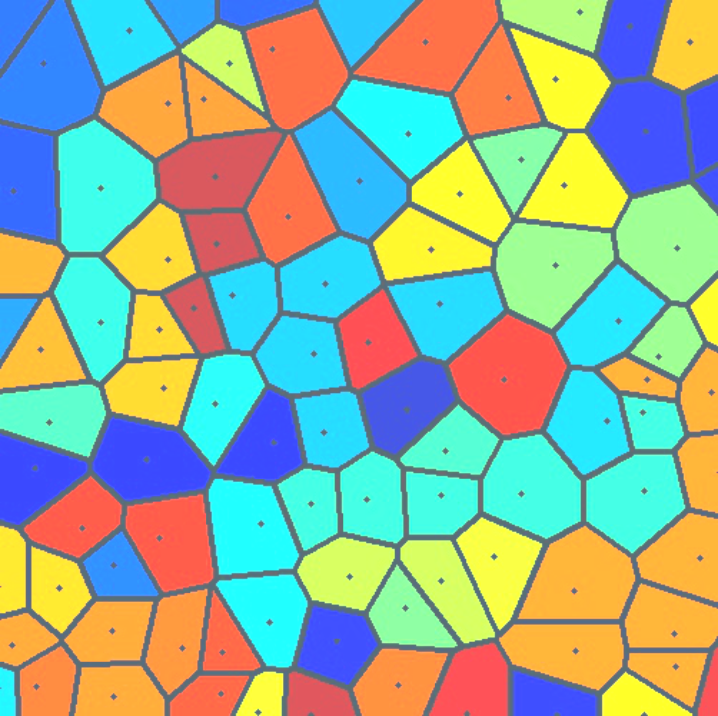
\includegraphics[width=0.3\textwidth]{fig7}
\end{figure}
Para finalizar o argumento pegue \(D\) como a  Voronoi cell da  órbita de qualquer ponto \(p \in M\). Note que pode sim ter dois elementos na mesma classe de equivalência dentro de \(D\). Porém, nesse caso eles devem ficar na fronteira \(\partial D\) já que \(G\) age por isometrias. Para concluir note que \(\pi|_{\operatorname{Int}D}\) é uma isometria, e portanto \(\operatorname{Vol}D=\operatorname{Vol}S^3/G\) como queriamos.
\item Lembre a pergunta: \textit{exibir uma sequência de variedades Riemannianas completas com curvatura constante igual a 1 de modo que a sequência dos volumes seja uma sequencia que converge a zero}. A resposta natural é \(S^3/G_q\) onde \(G_q\) é o grupo que determina o espaço lenticular, pudendo mudar o valor de \(r\) livremente desde que para cada \(q\) fique \(r\) primo relativo com \(q\).

	Então só falta mostrar que a curvatura secional de \(S^3/G\) é constante igual a 1, e que é completa. O último é imediato porque \(S^3\) é completa. Para ver o primeiro usamos de novo o exercício 10(b) que diz que para \(X,Y \in \mathfrak{X}(S^3/G)\), \(\sigma=\operatorname{span}\{X,Y\}\) e \(\overline{\sigma}=\operatorname{span}\{\overline{X}, \overline{Y}\}\),
\[\boxed{K(\sigma)=\overline{K}(\overline{\sigma})+\frac{3}{4}\left|\left[ \overline{X},\overline{Y} \right]^v\right|^2}\]
onde \(\overline{K}\) é a curvatura de \(S^3\), que \(1\). Ou seja, queremos ver que
\[\left[ \overline{X},\overline{Y} \right]^v=0.\]
Mas isso segue de que a ação é discreta! Temos uma descomposição \(TS^3 \cong \kappa \oplus  \pi^*T(S^3/G)\), onde \(\kappa\) é o kernel de \(\pi_*\). Como a dimensão do grupo é zero, a dimensão do espaço lenticular é 3, e o kernel dever ter dimensão zero. Então não tem componentes verticais em geral. (Então aprendi que a curvatura seccional é preservada em quocientes sob ações discretas.)
\end{enumerate}
\end{proof}

\begin{thing6}{Exercício 3}\label{exer:3}\leavevmode
Encontre um exemplo de variedade suave que admite uma métrica Riemanniana com curvatura escalar positiva, mas não admite uma métrica Riemanniana com Ricci positivo.
\end{thing6}

\begin{proof}[Solução]\leavevmode
	É parecida à solução de ``Hadamard não vale para curvatura escalar" que o Rafael diu na monitoria: pegue \(\mathbb{H}^{2}_{\frac{1}{100}}\), i.e. espaço de curvatura seccional constante negative e pequeníssima, e faça produto com uma esfera. Então a curvatura escalar é positiva porque é a suma dos pullbacks das curvaturas escalares, que coincidem com as curvaturas seccionais. Porém, a curvatura de Ricci, que também é a soma dos pullbacks das curvaturas de Ricci, não pode ser positiva porque em qualquer ponto podemos pegar um vetor cuja componente em \(S^2\) é zero, e a componente hiperbólica vai dar um número negativo. Para confirmar isso último 
	\iffalse é fácil de comprovar usando a fórmula de \(R\) para curvatura constante
\[\left<R(X,Y)Z,W\right>=c\Big(\left<X,W\right>\left<Y,Z\right>-\left<X,Z\right>\left<Y,W\right>\Big)\]
pois segue dela que
\begin{align*}
\operatorname{Ric}_{\mathbb{H}}(X,Y)&=\operatorname{tr}\Big(Z \mapsto R(Z,X)Y\Big)\\
&=\sum \left<R(E_i,X)Y,E_i\right>\\
&=\sum c \Big(\left<E_i,E_i\right>\left<X,Y\right>-\left<E_i,X\right>\left<Y,E_i\right>\\
&=c\sum \Big(n \left<X,Y\right>-\left<X,Y\right>\Big)\\
&=c(n-1)\left<X,Y\right>
\end{align*}
E aí lembrei\fi lembre a definição de \(\operatorname{Ric}\) negativo ou positivo: é a definição para uma forma bilinear, que está dada como o signo da forma avaliada no mesmo vetor nas duas entradas. Então só note que \(\operatorname{Ric}(X,X)=\sum K(E_i,X)<0\).

\end{proof}

\begin{thing6}{Exercício 4}\label{exer:4}\leavevmode
Encontre um exemplo de variedade suave que admite uma métrica Riemanniana com Ricci positivo, mas não admite uma métrica Riemanniana com curvatura seccional positiva.
\end{thing6}

\begin{proof}[Solução]\leavevmode
\(S^2\times S^1\), porque pelo teorema de Synge, se \(S^2\times S^1\) admitisse uma métrica com \(K>0\), teria que ter \(\pi_{1}(S^2 \times S^1)=\mathbb{Z}_2\) porque tem dimensão ímpar e é orientável. A métrica produto tem Ricci positivo já que \(\operatorname{Ric}S^2>0\), e, como no exercício anterior, sabemos que Ricci de um produto é a soma dos pullbacks das Ricci's em cada componente.
\iffalse
Então quero ver que o toro admite uma métrica com \(\operatorname{Ric}>0\). Pego a métrica plana, não porque todo se anula. Mas que tal a métrica como imersão dentro de \(\mathbb{R}^3\)? Uso Gauss… quero saber como é a segunda forma fundamental do toro… Ah, não! Uso o exercício 1 da lista 5… que ainda não resolvi… que diz que
\[\operatorname{Ric}(M_1 \times M_2)=\pi_1^*\operatorname{Ric}_1 + \pi_2^*\operatorname{Ric}2\]
e com isso acaba porque \(\operatorname{Ric}_{S^1}>0\).\fi
\end{proof}


\section{Variações de Energia}

\begin{thing6}{Exercício 5}\label{exer:5}\leavevmode
Sejam \((M^n,g)\) completa, conexa e com curvatura positiva e \(A,B\) subvariedades totalmente geodésicas e compactas tais que \(\dim A + \dim B \geq  n\). Mostre que \(A \cap B \neq  \varnothing\).
\end{thing6}

\begin{proof}[Solução]\leavevmode
	Suponha que a interseção não é vazia. Então existe uma geodésica minimizante não trivial que minimiza a distância entre \(A\) e \(B\). Sabemos que essa geodésica intersecta tanto \(A\) quanto \(B\) ortogonalmente. Queremos ver que \(E''(0)<0\), ou seja que \(\gamma\) não pode ser minimizante, uma contradição.

	Suponha que conseguimos construir uma variação de \(\gamma\) tal que todos os pontos iniciais \(f(s,0)\) estão em \(A\), e o mesmo acontece com os pontos finais, i.e. \(f(s,\ell) \in B\). Então as derivadas das curvas \(f(s,0)\) e \(f(s,\ell)\) em \(s=0\) são perpendiculares a  \(\gamma'(0)\) e \(\gamma'(\ell)\). Ou seja, temos que \(\left<\gamma'(0),\nabla_{\partial_s}V\right>|_{0}^\ell=0\).

	Suponha ainda que essa variação tem campo variacional paralelo. Então acabou porque a segunda fórmula da variação diz que
\[E''(0)=-\int_0^\ell \left<R_{\gamma'}V,V\right><0\]

Vamos construir essa variação. O passo inicial é fácil: pegamos qualquer vetor \(v \in T_a A\) e transportamos paralelamente ao longo de \(\gamma\) para obter o campo paralelo \(V \in \mathfrak{X}_\gamma\). Como \(A\) é totalmente geodésica, a variação \(f(s,t):=\operatorname{exp}_{\gamma(0)}(sV(0))\) fica dentro de \(A\).

Para concluir basta ver que \( V(\ell) \in T_bB\), já que \(B\) também é totalmente geodésica. Isso segue da última hipótese. Podemos realizar esse processo para cada vetor básico de  \(T_a A\), obtendo \(\dim A\) vetores linearmente independentes em \(T_bB\) (já que o transporte paralelo é uma isometria). Se nenhum deles ficasse em \(T_bB\), poderíamos construir um espaço de dimensão \(\dim A\) estritamente contido em \(T_b M\setminus T_b B\), absurdo pois isso implicaria que \(\dim A< \operatorname{codim} B\), porém, \(\dim A+ \dim B \geq n\).


\textbf{Edit.} Depois de reler a prova do exercício seguinte, parece que não era necessário usar que \(\gamma\) intersecta ortogonalmente \(A\) e \(B\), pois a variação que usei foi por geodésicas, então \(\nabla_{\partial_s}V=0\). Então fiquei com a dúvida de que parece que não usei compacidade de \(A\) e \(B\).
\iffalse
A segunda fórmula da variação da energia para variações próprias diz que
\[0<E''(0)=\int_0^\ell|V'|^2-\int_0^\ell \left<R_{\gamma'}V,\gamma'\right>\]
ou seja,
\[0<\int_0^\ell\left<R_{\gamma'}V,\gamma'\right><\int_0^\ell |V'|^2\]


	Vamos de novo. Pegue \(a\in A\) e uma geodésica \(\gamma\) com \(\gamma'(0) \in T_a A\). Então \(\gamma \subset A\). Vamos ver se consigo uma variação de \(\gamma\) que atinja \(B\). Pegue uma variação de \(\gamma\) fixando o ponto inicial. Obtemos
\[E''(0)=\int_0^d |V'|-\int_0^d\left<R_{\gamma'}V,\gamma'\right>+\left<\gamma',\nabla_{\partial_s}V\right>(d)\]



	Pegue \(a \in A\) e \(b \in B\), e \(\gamma\) geodésica minimizante que liga \(a\) a \(b\). O exercício acaba se mostramos que \(\gamma'(0)\in T_aA\). Suponha que \(\gamma'(0)\not \in T_aA\) e construamos uma variação própria de \(\gamma\) com menor energia que \(\gamma\)---uma contradição, pois \(\gamma\) é minimizante.

A segunda fórmula da variação da energia para variações próprias diz que
\[0<E''(0)=\int_0^\ell|V'|^2-\int_0^\ell \left<R_{\gamma'}V,\gamma'\right>\]
ou seja,
\[0<\int_0^\ell\left<R_{\gamma'}V,\gamma'\right><\int_0^\ell |V'|^2\]
Significa que \(V'\) não pode ser nulo. 
%Aqui tem uma ideia. Pegue um vetor \(v \in T_pM\) (ou \(T_pA\)?). Considere o transporte paralelo dele ao longo de \(\gamma\). A segunda fórmula da variação mostra que \(\gamma\) não é minimizante com respeito as curvas associadas a essa variação.
\end{proof}

\begin{proof}[Solução erradíssima]\leavevmode
	\textbf{Ideia.} Suponha que a interseção não é vazia e pegue um ponto nela e um vetor tangente a \(M\) nesse ponto. A geodésica associada ficara dentro de \(A\) quanto de \(B\). Agora considere uma variação por geodésicas dessa geodésica. O campo variacional é de Jacobi e concluímos que, se \(\gamma\) é minimizante,
	\begin{align*}
	E''(0)&\geq 0\\
0&\leq \int_0^a |\dot V|^2-\int_0^a\left<R_{\dot \gamma}V,V\right>\\
\int_0^a\left<R_{\dot \gamma}V,V\right>&\leq \int_0^a |\dot V|^2\\
-\int_0^a\left<\ddot V,V\right>&\leq \int_0^a |\dot V|^2\\
\int_0^a \left<\dot V,\dot V\right>-\int_0^a\left<\dot V,V\right>'&\leq \int_0^a |\dot V|^2\\
\left<\dot V(0),V(0)\right>& \leq \left<\dot V(a),V(a)\right>
	\end{align*}
	Como usar a curvatura sendo positiva? E como usar a hipótese da dimensão…
\fi\end{proof}

\begin{thing6}{Exercício 6}\label{exer:6}\leavevmode
Seja \(M^{2n}\) uma variedade Riemanniana de dimensão par, completa, orientável e com curvatura seccional \(K>0\). Seja \(\gamma\) uma geodésica fechada em \(M\) de comprimento \(\ell(\gamma)\). Mostre que existem curvas livremente homotópicas a \(\gamma\) em \(M\), arbitrariamente próximas de \(\gamma\), que possuem comprimento menor que \(\ell(\gamma)\).

\textbf{Sugestão.} Estude variações de \(\gamma\) com campo variacional paralelo ao longo de \(\gamma\).
\end{thing6}

\begin{proof}[Solução]\leavevmode
Considere qualquer vector unitário ortogonal a \(\dot \gamma\), defina \(V\in \mathfrak{X}_{\gamma}''\) como sendo o transporte paralelo de \(v\) ao longo de \(\gamma\). Note que \(\dot V=0\). Defina a variação \(f(s,t)=\operatorname{exp}_{\gamma(t)}sV(t)\). Note que \(\nabla_{\partial_s}f_s=0\).

A segunda fórmula da variação nos diz que
\[E''(0)=-\int_0^a \left<R_{\dot \gamma}V,V\right>=-\int_0^a K<0\]
já que \(K>0\). Como \(\gamma\) é uma geodésica, temos que para \(s\) pequeno
\[\frac{1}{a}\ell^2(c^s)\leq E(s) < E(0)= \frac{1}{a}\ell^2(\gamma)\]
Note que essa variação pode não preservar o fechamento das curvas. Para resolver isso olhemos ao seguinte desenho:
\begin{figure}[H]
	\centering
	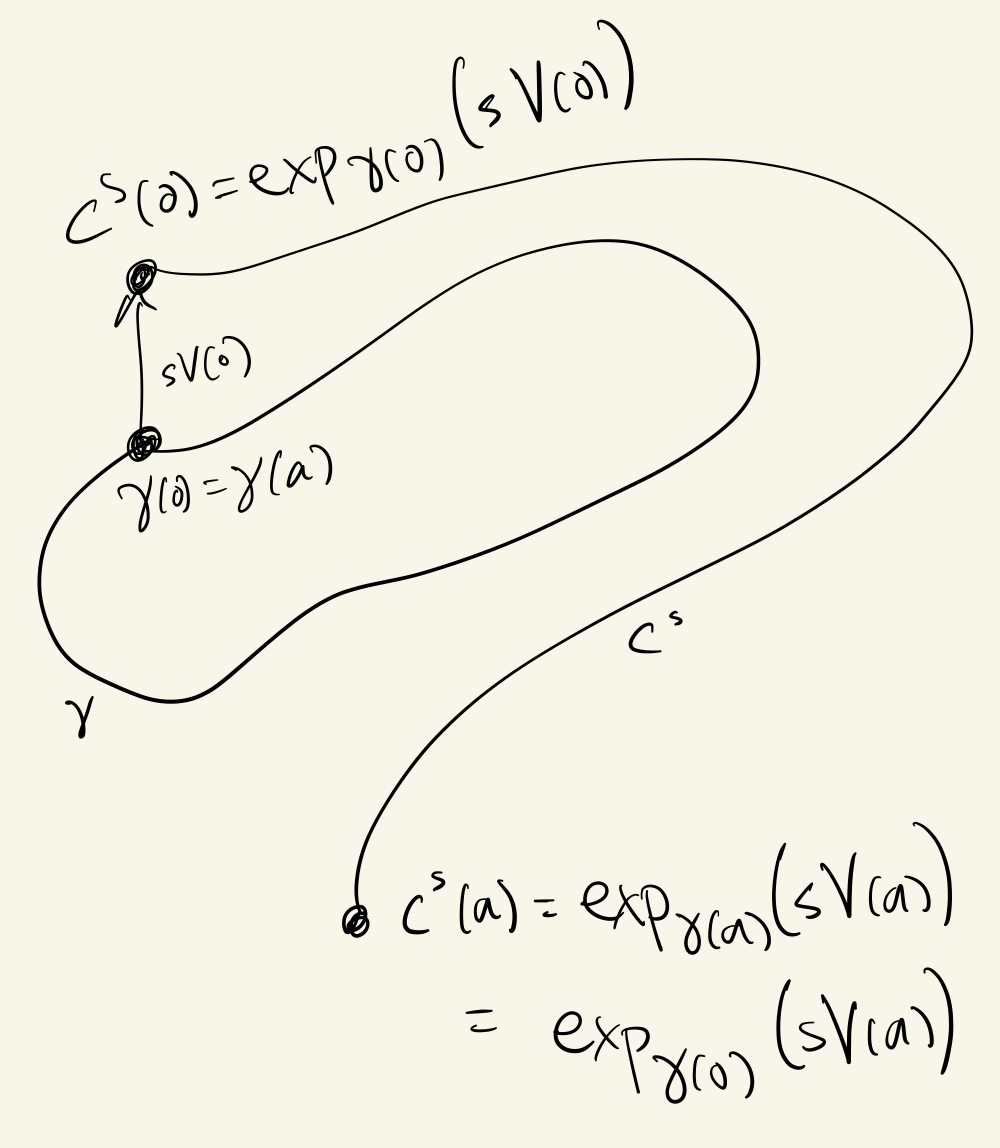
\includegraphics[width=0.5\textwidth]{fig6}
\end{figure}
Fica claro que se \(V(0)=V(a)\) as curvas \(c^s\) são fechadas para toda \(s\). Então a condição que precisamos é que
\[P^\gamma_{0,a}V(0)=V(a)\]
onde \(P\) é o transporte paralelo. Dito de outra forma, basta ver que \(P\) tem um ponto fixo---além de \(\gamma'(0)=\gamma'(a)\), que já é um ponto fixo. Esse argumento é uma imitação da prova do teorema de Weinstein: como \(P\) preserva orientação, o determinante dele deve ser positivo, ou seja, o produto dos seus autovalores deve ser positivo. Restringindo-nos ao subespaço \(\gamma'(0)^\perp\), que tem dimensão ímpar, concluímos que para que o produto dos autovalores de \(P\) seja positivo, deve ter pelo menos um que seja \(1\).
\end{proof}
\iffalse
\begin{proof}[Solução intento antes da aula de Weinstein]\leavevmode
Seguindo a sugestão pegue \(v \in T_pM\) unitário e ortogonal a \(\dot \gamma\), e considere o transporte paralelo dele \(V \in \mathfrak{X}'_\gamma\). Isso nos dá uma família de curvas livremente homotópicas a \(\gamma\) (sem fixar extremos). A segunda fórmula da variação nos diz que
\[\frac{d^2}{ds^2}E(s)\Big|_{s=0}=\cancelto{0}{\int_a^b |\dot V|^2}-\int_a^b \left<R(V,\dot \gamma)\dot \gamma,V\right>+\left<\nabla_{\partial_s}V,\dot \gamma\right>|_{a}^b\]
Note que como pegamos \(v \perp \dot \gamma\) e o transporte paralelo preserva o angulo, o termo com a curvatura é exatamente a curvatura seccional em \(\operatorname{span}\{V,\dot \gamma\}\), que deve ser positiva por hipótese.

%Para concluir o exercício bastaria argumentar que o termo \(\left<\nabla_{\partial_s}V,\dot \gamma\right>|_{a}^b\) se anula, já que sabemos que uma geodésica é minimizante se e somente se é um ponto mínimo de \(E\) ({\color{2}caveat:} realmente sabemos isso quando \(E\) está restringido ao subespaço de curvas diferenciáveis por partes fixando os extremos, que não é nosso caso).

Agora note que o termo \(\left<\nabla_{\partial_s}V,\dot \gamma\right>|_{a}^b\) se anula. Isso segue do lema de simetria:
\begin{align*}0=\partial_s\left<V,\dot \gamma\right>&=\left<\nabla_{\partial_s}V,\dot \gamma\right>+\left<V,\nabla_{\partial_s}\dot \gamma\right>\\
	&=\left<\nabla_{\partial_s}V,\dot \gamma\right>+\left<V, \nabla_{\partial_s}\nabla_{\partial_t}\Gamma(s,t)\right>\qquad \text{\(\Gamma\) é a variação} \\
&=\left<\nabla_{\partial_s}V,\dot \gamma\right>+\left<V,\nabla_{\partial_t}\nabla_{\partial_s}\Gamma(s,t)\right>\qquad \text{lema de simetría} \\
&=\left<\nabla_{\partial_s}V,\dot \gamma\right>+\cancelto{0}{\left<V,\dot V\right>}\qquad \qquad \qquad  \text{\(V\) paralelo} 
\end{align*}
{\color{2}Acho que tá errado! Porque essa função não está definida em todo o domínio da variação, e sim apenas sobre a curva!}

Então concluímos que
\[E''(0)<0\]
Isso implica que \(\gamma\) é um máximo da energia, ou seja, existe uma vizinhança de \(0\) tal que para todo \(s\) nessa vizinhança,
\[E(s)<E(0)\]
\end{proof}
\fi



\clearpage
\begin{minipage}{\textwidth}
	\begin{minipage}{1\textwidth}
		{\small Prof. Luis Florit\hfill Daniel González Casanova Azuela}
		
		{\small Monitor. Ivan Miranda\hfill\href{https://github.com/danimalabares/rg}{github.com/danimalabares/rg}}
	\end{minipage}
\end{minipage}\vspace{.2cm}\hrule

\vspace{10pt}
{\huge Lista 7}
\addcontentsline{toc}{section}{Lista 7}
\begin{thing6}{Exercício 1}[Lema de Klingenberg, \cite{doc}, Cap. X, Exer. 1]\label{exer:1}\leavevmode
	Seja \(M\) uma variedade Riemanniana completa com curvatura seccional \(K \leq  K_0\) onde \(K_0\) é uma constante positiva. Sejam \(p,q \in M\) e seja \(\gamma_0\) e \(\gamma_1\) duas geodésicas distinas unindo \(p\) a \(q\) com  \(\ell(\gamma_0) \leq  \ell(\gamma_1)\). Admita que \(\gamma_0\) é homotópica a \(\gamma_1\), isto é, existe uma família contínua de curvas \(\alpha_t\), \(t \in [0,1]\) tal que \(\alpha_0 = \gamma_0\) e \(\alpha_1=\gamma_1\). Prove que existe \(t_0 \in [0,1]\) tal que
	\[\ell(\gamma_0)+\ell(\alpha_{t_0}) \geq  \frac{2\pi}{\sqrt{K_0} }\]
\end{thing6}

\begin{proof}[Solução]\leavevmode
Primeiro vou mostrar como usar o teorema de Rauch para assegurar que para qualquer \(p \in M\), a exponencial em \(p \in M\) não possui pontos críticos na bola de raio \(\pi/\sqrt{K_0}\) centrada em \(0 \in T_pM\).

O seguinte argumento mostra que qualquer geodésica \(\gamma\) com velocidade unitária partindo de \(p\) não possui pontos conjugados antes de alcançar comprimento \(\pi/\sqrt{K_0}\). Fixe um campo de Jacobi \(J \in \mathfrak{X}_\gamma^J\) tal que \(J(0)=0\) e \(\left<J,\gamma'\right>=0\). Para aplicar Rauch, considere uma geodésica unitária \(\tilde{\gamma}\) em \(S^n_{K_0}\), a esfera de curvatura constante \(K_0\), e um campo de Jacobi  \(\tilde{J}\in\mathfrak{X}_{\tilde{\gamma}}^J\) tal que \(\tilde{J}(0)=0\), \(\left<\tilde{J},\tilde{\gamma}'\right>=0\) e \(|J'(0)|=|\tilde{J}'(0)|\). (\(\tilde{J}\) existe por ser a solução da equação de Jacobi junto com a condição de ortogonalidade com \(\tilde{\gamma}'\).) Como \(K \leq K_0\), pelo lema de Rauch concluímos que \(0 \leq  |\tilde{J}|\leq |J|\) para \(t <\pi/\sqrt{K_0}\).

	Agora vou argumentar por que isso assegura que \(\operatorname{exp}_p\) não pode ter pontos críticos em \(p \in M\). Por contrapositiva, suponha que \(\operatorname{exp}_p\) tem um ponto crítico em \(v \in T_pM\) e vamos mostrar que existe um ponto conjugado  \(q\) a \(p\) ao longo de \(\gamma\). Como \(v\) é um ponto crítico de \(\operatorname{exp}_p\), existe um vetor não nulo \(w \in \ker d_v \operatorname{exp}_p\). Considere uma curva \(c(s)\) tal que \(c(0)=v\) e \(c'(0)=w\). Temos a seguinte variação por geodésicas de \(\gamma\): \(\gamma_{c(s)}(t)=\operatorname{exp}_{p}(tc(s))\). Note que em \(t=0\) todas as geodésicas ficam em \(p\), pelo que o campo variacional \(J\) se anula em \(p\). O fato de que \(d_v \operatorname{exp}_p(w)=\frac{d}{ds}\Big|_{s=0}\operatorname{exp}_p(c(s))=0\), é exatamente o fato de que o campo variacional \(J\) se anula em \(q=\gamma_v(1)\).

\begin{figure}[H]
	\centering
	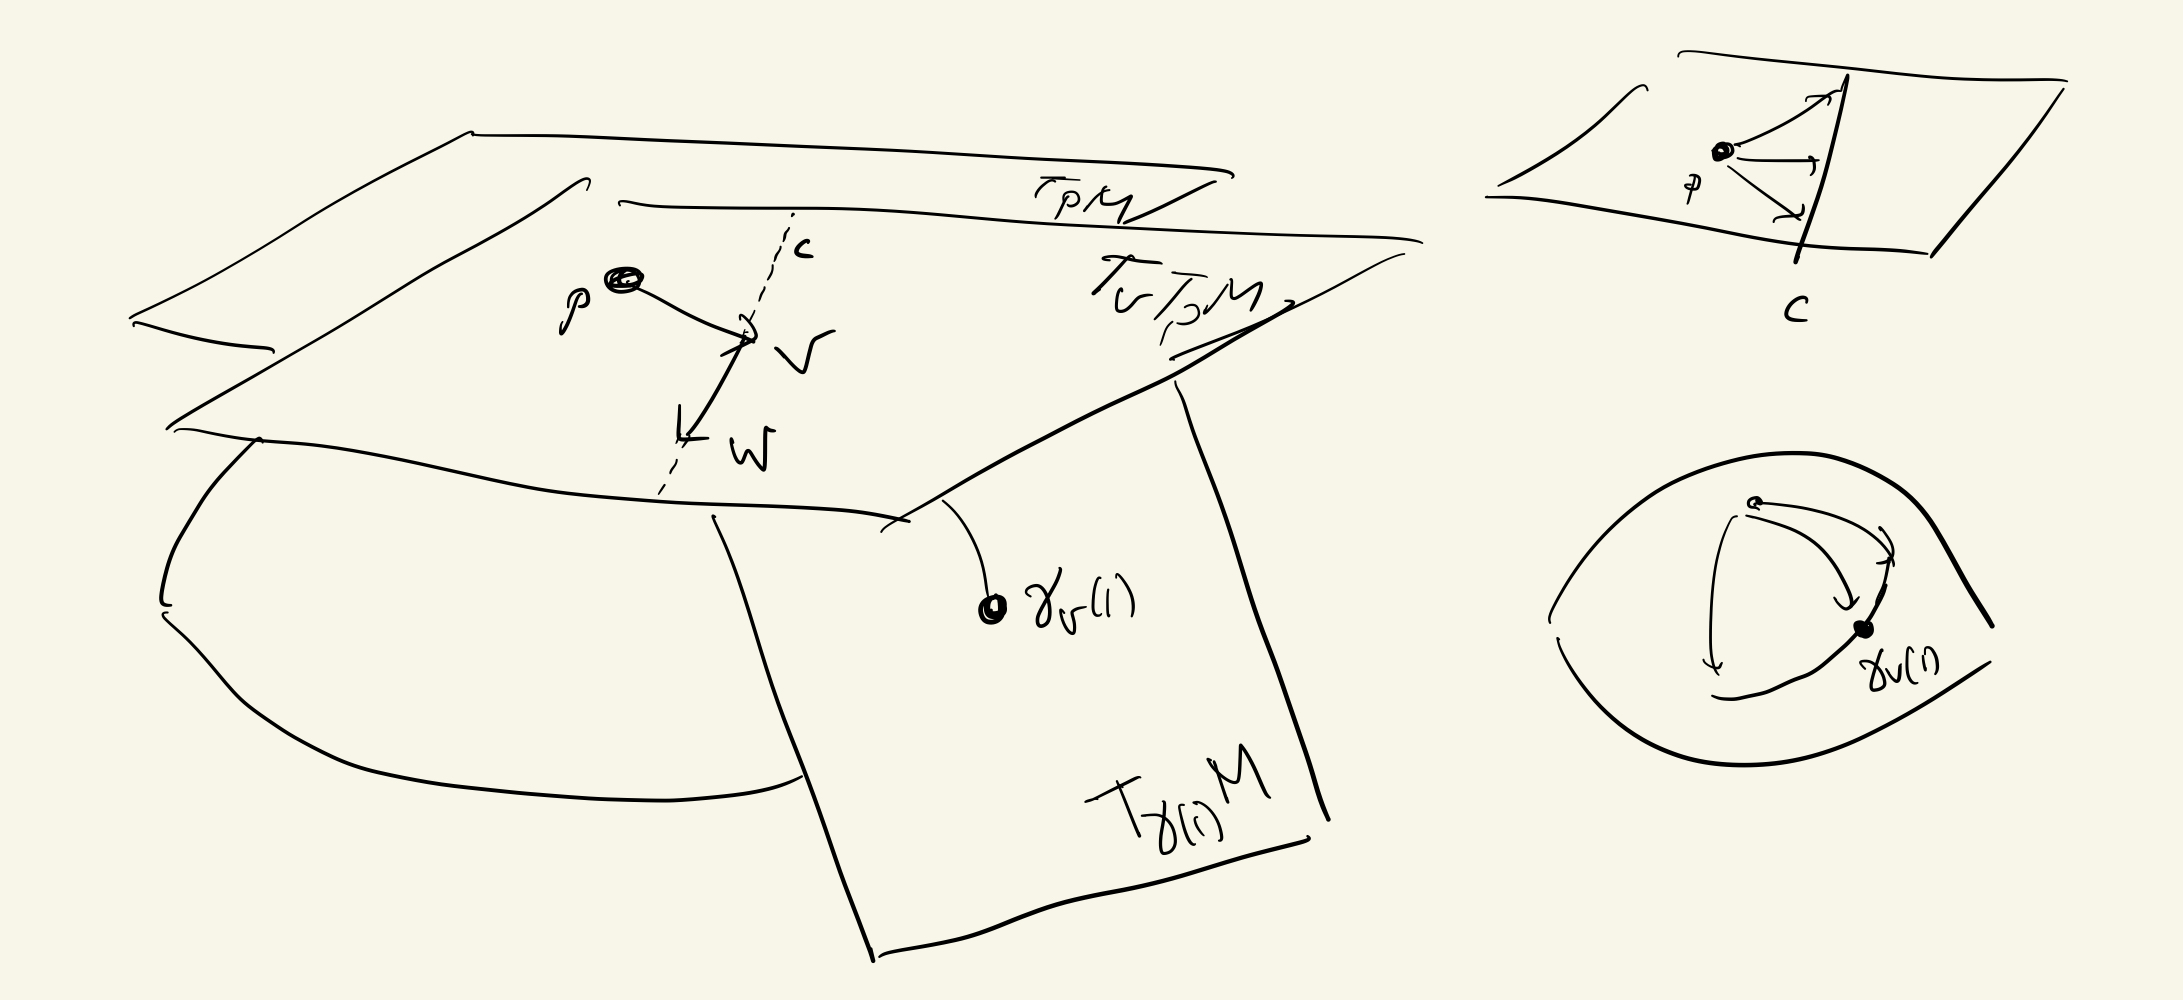
\includegraphics[width=0.75 \textwidth]{fig8}
\end{figure}
Portanto, \(\operatorname{exp}_p\) é um difeomorfismo local sobrejetivo em \(B_{\pi/\sqrt{K_0}}\), mas pode não ser injetivo:
\begin{figure}[H]
	\centering
	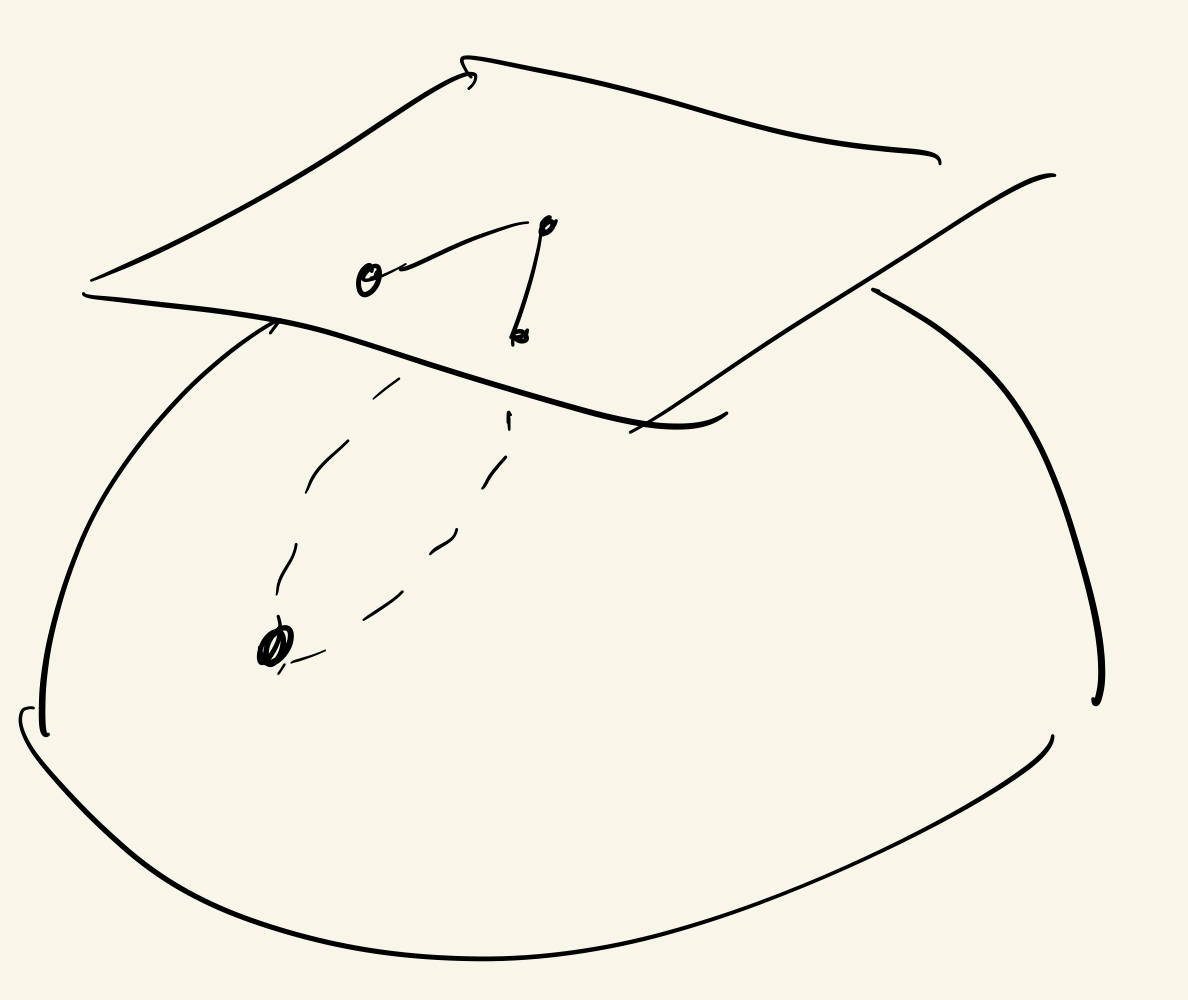
\includegraphics[width=0.4\textwidth]{fig10}
\end{figure}
Note que podemos levantar tanto \(\gamma_0\) quanto \(\gamma_1\) por ser geodésicas, i.e. pegamos os vetores velocidade de cada uma e as linhas que eles geram no espaço tangente a \(p\); é claro que essas curvas são levantamentos de \(\operatorname{exp}_p\). Note que se levantássemos a homotopia completa, necessariamente \(\gamma_0=\gamma_1\). Isso segue simplesmente de que não pode ter uma família contínua de curvas começando em um ponto e terminando em outro.

\begin{thing7}{Dúvida}\leavevmode
Como estão construídos os levantamentos das curvas perto de \(\gamma_0\)? Em \cite{doc} simplesmente se afirma que é claro que podemos levantar as curvas perto de \(\gamma_0\), mas que não será possível levantar a homotopia completa.

Eu só sei que podemos levantar \(\gamma_0\) e \(\gamma_1\) usando as velocidades delas e o fato de que \(\operatorname{exp}_p\) manda esses vetores em essas curvas; mas as outras curvas da homotopia não são geodésicas e esse argumento não aplica.
\end{thing7}

Para entender melhor a construção consultei \cite{docsu}. Cap. 5., sec. 6. Prop. 2, que estabelece a existência e unicidade dos levantamentos de curvas (ou ``caminhos") \textit{no caso das aplicações de recobrimento}. A prova da unicidade parece válida para homeomorfismos locais, e como é parecida ao argumento de achar um conjunto aberto e fechado dentro do intervalo (como na sugestão do nosso exercício), achei bom passar em limpo. Mas \textbf{pode pular}, essa prova não é importante para a discussão que segue.

\begin{thing7}{Unicidade de levantamentos para aplicações de recobrimentos}\leavevmode
	Seja \(\pi:\tilde{B}\to B\) é homeomorfismo local, \(\alpha:[0,\ell] \to B\) um caminho em \(B\) e \(\tilde{p}_0 \in \tilde{B}\) um ponto de \(\tilde{B}\) tal que \(\pi(\tilde{p}_0)=\alpha(0)=p_0\). Se existe um levantamento \(\tilde{\alpha}:[0,\ell] \to \tilde{B}\) de \(\alpha\) com origem em \(\tilde{p}_0\), \textbf{ele é único}.
\end{thing7}

\begin{proof}\leavevmode
	Suponha que existe outro levantamento \(\tilde{\beta}:[0,\ell] \to \tilde{B}\) de \(\alpha\) com origem em \(\tilde{p}_0\). Seja \(A \subset[0,\ell]\) o conjunto de pontos onde \(\tilde{\alpha}\) e \(\tilde{\beta}\) coincidem. Ele é fechado porque se pegamos uma sequência de pontos dentro de ele, por continuidade tanto de \(\tilde{\alpha}\) quanto de \(\tilde{\beta}\) o ponto limite irá ficar dentro de \(A\).

	Para ver que é aberto considere um ponto \(t \in A \subset I\). Vamos mostrar que existe uma vizinhança dele totalmente contida em \(A\). Defina \(\tilde{p}:=\tilde{\alpha}(t)=\tilde{\beta}\) (que vale porque pegamos \(t \in A\)). Pegue uma vizinhança \(V\) de \(\tilde{p}\) onde \(\pi\) seja um homeomorfismo. Como \(\tilde{\alpha}\) e \(\tilde{\beta}\) são contínuas, as imagens inversas de \(V\) sob \(\tilde{\alpha}\) e \(\tilde{\beta}\) podem ser intersectadas para produzir uma vizinhança \(I_t\) de \(t\).

	Só falta ver que \(\tilde{\alpha}\) e \(\tilde{\beta}\) coincidem em \(I_t\). Como \(\tilde{\alpha}\) e \(\tilde{\beta}\) são levantamentos, sabemos que \(\pi \circ \tilde{\alpha}=\pi \circ \tilde{\beta}\). Como \(\pi\) é um homeomorfismo em \(V\), podemos inverter ele para concluir que \(\tilde{\alpha}=\tilde{\beta}\) nessa vizinhança.

	\begin{figure}[H]
		\centering
		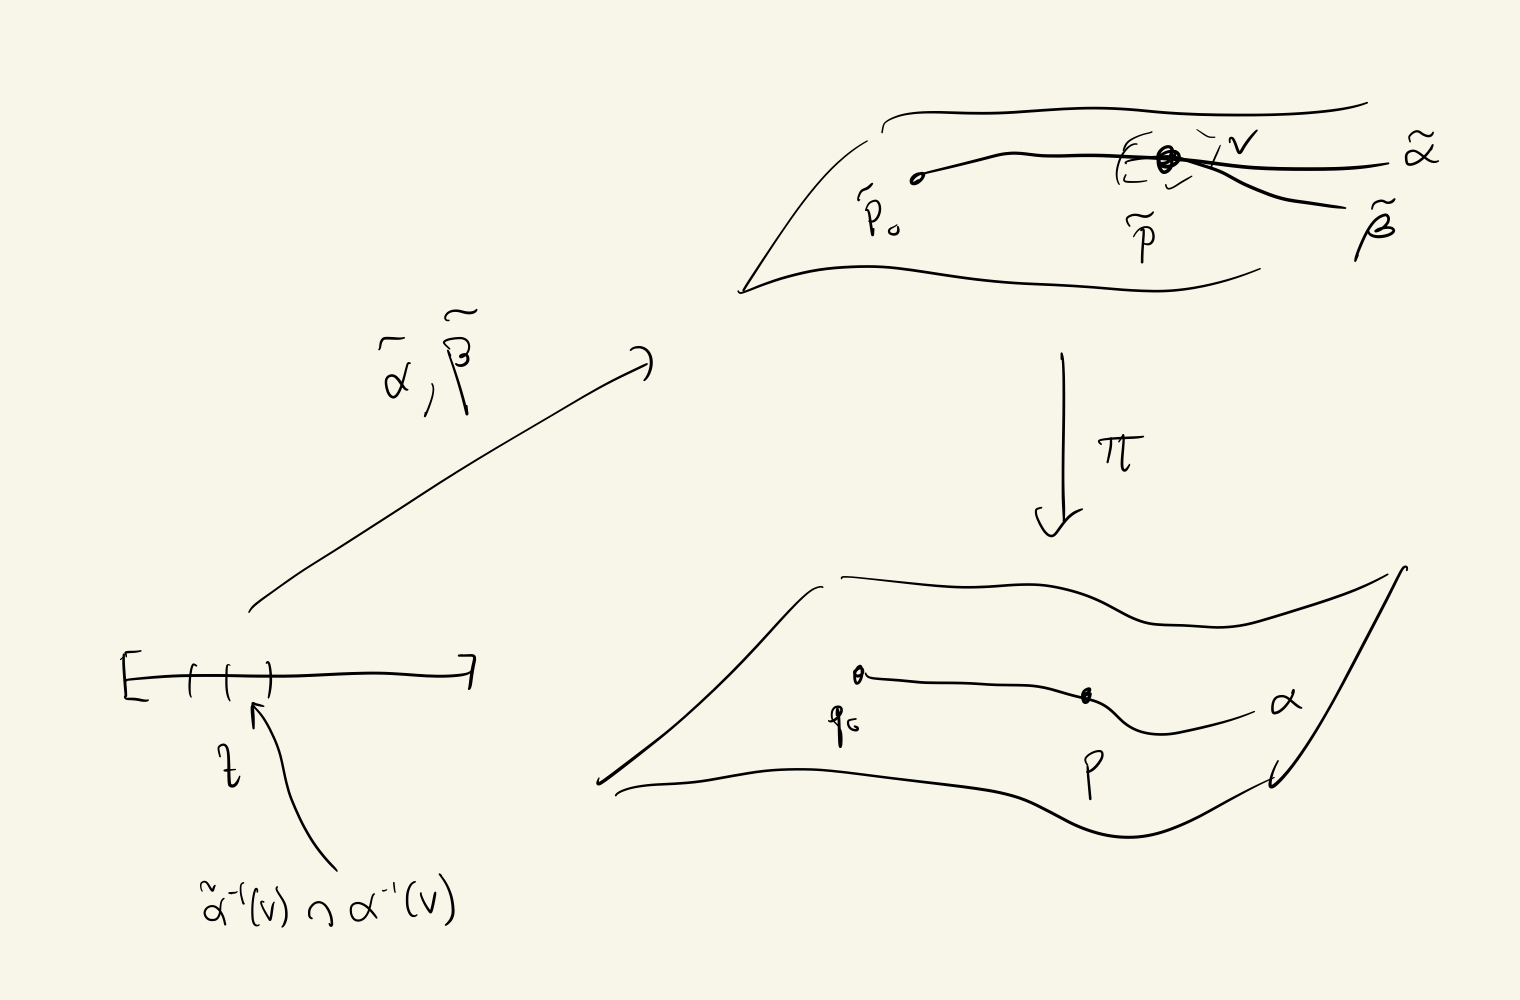
\includegraphics[width=0.7\textwidth]{fig13}
		\caption*{}
	\end{figure}
\end{proof}

Porém o que realmente nos compete aqui é a existência dos levantamentos. O problema é que isso não vale para difeomorfismos (ou homeomorfismos) locais arbitrários. A prova de existência de levantamentos em \cite{docsu} para aplicações de recobrimento pode ser resumida assim:
\begin{enumerate}[label=(\alph*)]
\item Para cada \(t \in I\) podemos considerar uma \textbf{vizinhança distinguida} de \(\alpha(t)\). Ou seja, uma vizinhança de \(V_t \ni \alpha(t)\) tal que \(\pi^{-1}(U_t)\) é uma união disjunta de abertos de \(\tilde{M}\) onde \(\pi\) se restringe a um homeomorfismo. Note que isso não existe em nosso caso; apenas podemos garantir a existência de uma vizinhança de \(\alpha(t)\) onde \(\pi\) se restringe a um difeomorfismo.
\item Usando a compacidade do intervalo junto com a continuidade de \(\alpha\) podemos cobrir o caminho \(\alpha(I)\) com uma quantidade finita de abertos.
\item Considere o primeiro deles, \(I_0\). Como \(\pi\) se restringe a um homeomorfismo nessa vizinhança, podemos levantar esse pedacinho da curva \(\alpha\) como sendo simplesmente a preimagem de \(\alpha(I_0)\) sob \(\pi\) a algum dos abertos disjuntos que são a preimagem da vizinhança distinguida. Isso vale para nosso difeomorfismo local na preimagem do aberto em que \(\operatorname{exp}_p\) é um difeomorfismo.
\item Considere agora \(I_1\), o seguinte intervalo. Deve existir um ponto \(t \in I_1 \cap I_0\). A imagem inversa de \(\pi\) em \(V_1\) é uma união disjunta de abertos distinguidos, \textbf{um dos quais deve intersectar \(V_0\)} simplesmente por definição de conjunto. O lance é que \textbf{toda}  a imagem inversa de \(V_0\) é uma união de abertos distinguidos e por isso podemos garantir que um deles intersecta o aberto distinguido onde começamos nosso levantamento.

	No caso de \(\operatorname{exp}_p\), embora podemos garantir que existe um aberto onde \(\operatorname{exp}_p\) se restringe a um homeomorfismo, não temos como garantir que essa vizinhança intersecta vizinhança onde começou o levantamento. 

Continuando com a construção, como \( \pi\) se restringe a um homeomorfismo em \(V_1\) podemos definir um levantamento novamente como a imagem inversa sob \(\pi\).

Como já provamos unicidade e \textbf{os levantamentos coincidem num ponto}, o segundo levantamento coincide com o primeiro na interseção \(I_0 \cap I_1\).
\item Podemos fazer esse processo para o número de intervalos, que é finito, obtendo um único levantamento de \(\alpha\).
\end{enumerate}

Finalmente vamos dar uma olhada à prova do levantamento de homotopias para homeomorfismos locais com a propriedade de levantamento de curvas, Prop. 3 em \cite{docsu}, Cap. 5, Sec. 6. A estratégia é clara: dada uma homotopia no espaço base, definimos a homotopia no espaço total como sendo o levantamento de cada uma das curvas na base usando fortissimamente a propriedade de levantamento de curvas. A prova consiste em provar unicidade (análoga à unicidade de levantamentos de curvas) e a continuidade da homotopia levantada.

Então parece que essa prova não vai ajudar no nosso caso: \textbf{não vejo como garantir o levantamento de nenhuma curva além de \(\gamma_0\) ou \(\gamma_1\), mesmo que esteja perto de \(\gamma_0\) com respeito ao parâmetro da homotopia}.

Por fim, esse problema queda resolvido se fixamos nossa atenção só nos abertos que obtemos usando que \(\operatorname{exp}_p\) é um difeomorfismo local ao longo de \(\gamma_0\). Desse jeito conseguimos construir por pedaços, usando que \(\operatorname{exp}_p\) é um homeomorfismo em cada aberto e a unicidade dos levantamentos em cada interseção, um levantamento de qualquer curva que esteja completamente contida na união dos abertos gerados ao longo de \(\gamma_0\).

Note que esse processo pode ser feito de novo para qualquer curva que já tenhamos conseguido levantar. De fato, se todas as curvas da homotopia estivessem contidas em \(B_{\pi/\sqrt{K_0}}(p) \subset M\), poderíamos levantar toda a homotopia como mostrarei a seguir.

%Considere o conjunto \(C\) de todas as curvas levantáveis em \(M\), i.e. a união dos ``traços" \(\alpha_t(I)\) para cada \(t \in A\). Vamos mostrar que é um conjunto fechado. Considere uma sequência \(\gamma(t_n) \subset C\) convergente a \(\gamma(t_0) \in M\). Como a homotopia  \(H\) é uma função contínua e \(\{t_n\}\cup  \{t_0\}\) é um conjunto fechado …?

Usando o esquema usado multiples vezes por Manfredo, defina \(A \subset I\) como sendo o conjunto de parâmetros de curvas que podem ser levantadas. Vamos mostrar que esse conjunto é aberto e fechado, e portanto é todo \(I\).

Fiz uma tentativa de mostrar que \(A\) é fechado pegando uma sequência \(t_n \subset A\) convergente a \(t_0 \in I\). Mas não funcionou porque ter pontos perto do parâmetro limite não assegura que as curvas na imagem estejam perto; a homotopia não é uma função contínua definida no intervalo, e projetar do quadrado \(I \times I\) ao intervalo perde informação.

Então voltei à sugestão de \cite{doc}. Suponha ainda que existe um \(\varepsilon>0\) que tal que o levantamento de toda curva que consiga ser levantada esteja a distância \(\geq \varepsilon\) do bordo de \(B_{\pi/\sqrt{K_0}}\subset T_pM\). Mas… \textbf{mesmo supondo isso não sei como levantar cada curva} 


Agora o plano é usar a continuidade da homotopia \(H\) via ``preimagem de fechado é fechado".


Mas isso está malíssimo porque fica no \(T_pM\). Então melhor suponha que existe \(\varepsilon\) toda curva que consiga ser levantada esteja a distância \(\geq \varepsilon\) de \(B_{\pi/\sqrt{K_0}}\subset M\). Então as curvas levantáveis estão dentro de um 

O conjunto de curvas levantadas está 


Como a homotopia \(H:[0,1]\times[0,1]=I^2 \to M\) é uma função contínua, a imagem inversa de qualquer aberto de \(M\) é um aberto de \(I^2\). Considere para cada curva em \(A\), i.e. cada curva que já conseguimos levantar, uma coberta aberta finita por abertos onde \(\operatorname{exp}_p\) é um difeomorfismo. Pegue a preimagem sob \(H\) da união de todos esses abertos, que é um aberto de \(I^2\). Agora projete esse aberto ao intervalo de parâmetros que varia as curvas da homotopia. Esse é um aberto \(V\) de \(I\) que contém \(A\).

 Considere a curva \(\alpha_{t_0}\) e uma vizinhança dela 





Agora podemos continuar seguindo a sugestão dada em \cite{doc}. Agora queremos provar que para qualquer \(\varepsilon\) existe um levantamento \(\alpha_\varepsilon\) que contém pontos a distância menor que \(\varepsilon\) do bordo da bola \(B_{\pi/\sqrt{K_0}}(0)\subset T_pM\) .

Suponha que existe um \(\varepsilon\) tal que todo levantamento \(\tilde{\alpha}_t\) está a distância \(\geq \varepsilon\) desse bordo. Como na prova da unicidade dos levantamentos, defina \(A \subset [0,1]\) como sendo o conjunto de parâmetros \(t\) para os quais existe um levantamento de \(\alpha_t\).

Sabemos que \(A\) é não vazio e contém uma vizinhança aberta \(V\) de 0. Considere uma sequência \(t_n\) dentro de \(V\) que convirja a \(t_0 \in I\). Considere uma vizinhança aberta de \(t_0\) e um ponto 


\iffalse
\begin{figure}[H]
	\centering
	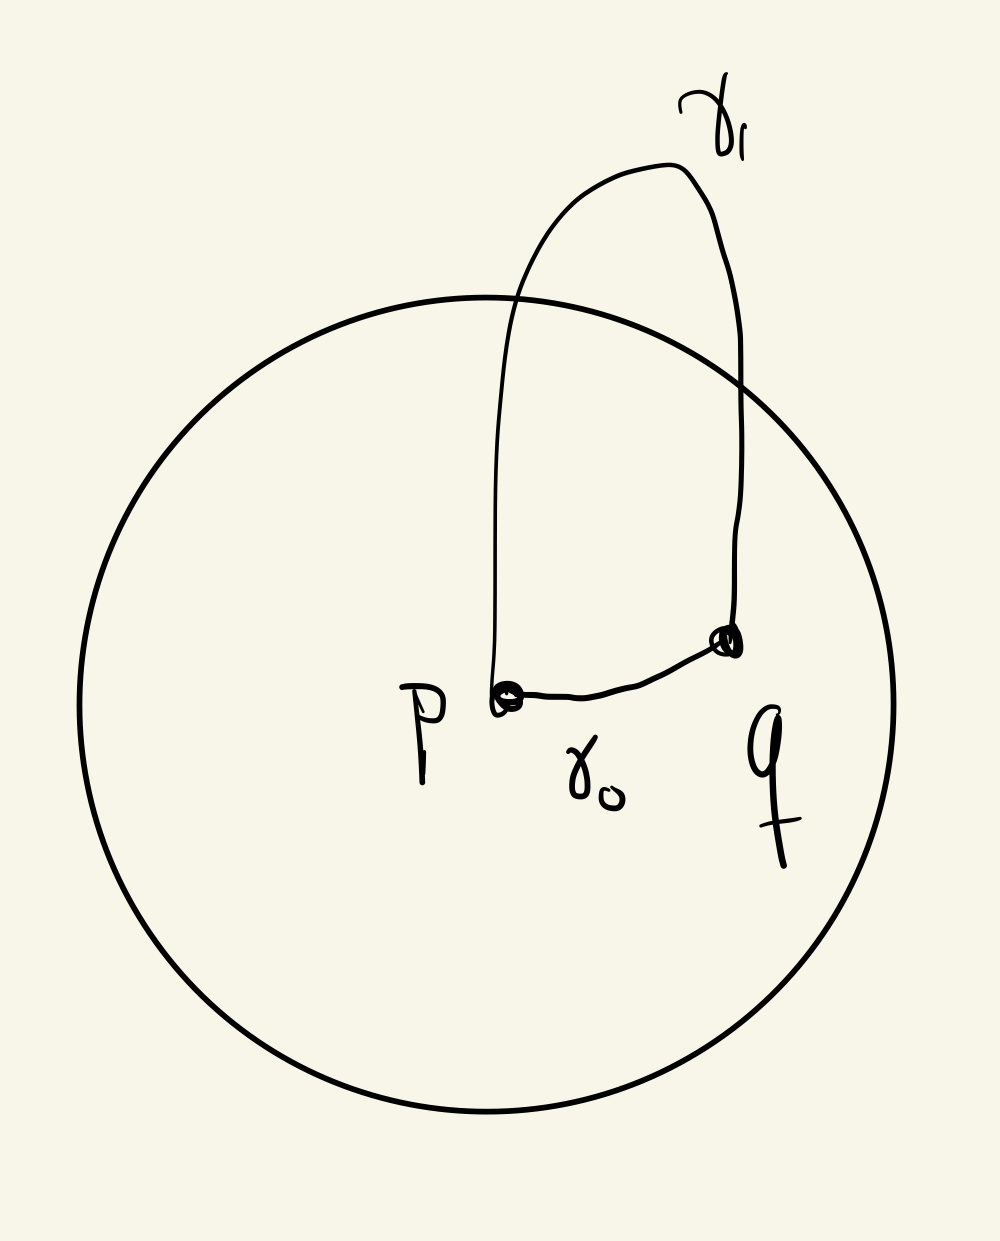
\includegraphics[width=0.3\textwidth]{fig9}
\end{figure}

Note que esse processo pode ser feito de novo para qualquer curva que já conseguimos levantar. De fato, se todas as curvas da homotopia estivessem contidas em \(B_{\pi/\sqrt{K_0}}(p) \subset M\), poderíamos levantar toda a homotopia como mostrarei a seguir.

Usando o esquema usado multiples vezes por Manfredo, defina \(A \subset I\) como sendo o conjunto de parâmetros de curvas que podem ser levantadas. Vamos mostrar que esse conjunto é aberto e fechado, e portanto é t odo \(I\).

Como a homotopia \(H:[0,1]\times[0,1]=I^2 \to M\) é uma função contínua, a imagem inversa de qualquer aberto de \(M\) é um aberto de \(I^2\). Considere para cada curva em \(A\), i.e. cada curva que já conseguimos levantar, uma coberta aberta finita por abertos onde \(\operatorname{exp}_p\) é um difeomorfismo. Pegue a preimagem sob \(H\) da união de todos esses abertos, que é um aberto de \(I^2\). Agora projete esse aberto ao intervalo de parâmetros que varia as curvas da homotopia. Esse é um aberto \(V\) de \(I\) que contém \(A\).

Pegue uma sequência \(t_n \subset A\) convergente a \(t_0 \in I\). Considere a curva \(\alpha_{t_0}\) e uma vizinhança dela 



\fi

\end{proof}

\begin{thing6}{Exercício 2}[\cite{doc}, Cap. X, Exer. 2]\label{exer:2}\leavevmode
Use o lema de Klingenberg do exercício anterior para provar o Teorema de Hadamard.
\end{thing6}

\begin{proof}[Solução]\leavevmode
	Suponha que \(M\) é uma variedade completa, simplesmente conexa e com curvatura positiva. Por completitude, sabemos que para qualquer \(p \in M\) o domínio de \(\operatorname{exp}_p\) é todo \(T_pM\). Como \(K \leq 0\) sabemos que \(M\) não pode ter pontos conjugados, de modo que  \(\operatorname{exp}_p\) é um difeomorfismo local. Também por completitude sabemos que \(\operatorname{exp}_p\) é sobrejetiva: qualquer ponto \(q\) está ligado a \(p\) mediante uma geodésica, e essa geodésica coincide com uma geodésica partindo de \(p\) dada como a imagem de uma reta em \(T_pM\) sob \(\operatorname{exp}_p\).

	Portanto, o desafio é provar que \(\operatorname{exp}_p\) também é injetiva. Suponha que não é o caso, i.e. considere dois pontos \(v_1\) e \(v_2\) em \(T_pM\) tais que \(\operatorname{exp}_pv_1=\operatorname{exp}_pv_2:=q\). As imagens das retas geradas por \(v_1\) e \(v_2\) sob \(\operatorname{exp}_p\) são duas geodésicas \(\gamma_1\) e \(\gamma_2\) em \(M\) ligando \(p\) e \(q\).

	Como \(M\) é simplesmente conexa, existe uma homotopia entre \(\gamma_1\) e \(\gamma_2\). Podemos aplicar o lema de Klinenberg para obter uma curva \(\alpha_{K_0}\) tal que
	\[\ell(\gamma_1)+\ell(\alpha_{K_0}) \geq 2\pi/\sqrt{K_0}\]
para qualquer \(K_0>0\). Isso mostra que o comprimento das curvas na homotopia não está limitado, o que não é possível já que a homotopia é uma função contínua definida em um compacto, pelo qual a sua imagem debe ser compacto e portanto limitado.
\end{proof}

\begin{thing7}{Dúvida}\leavevmode
Teve um comentário discutido na monitoria com respeito à necessidade de usar o teorema de Whitney para assegurar que a homotopia seja suave: não usei esse fato.
\end{thing7}

\begin{thing6}{Exercício 3}[\cite{doc}, Cap. X, Exer. 3]\label{exer:3}\leavevmode
Seja \(M\) uma variedade Riemanniana completa com curvatura seccional não positiva. Prove que
\[|(d \operatorname{exp}_p)_v(w)|\geq |w|\]
para todo \(p \in M\), \(v \in T_pM\) e \(w \in T_v(T_pM)\).
\end{thing6}

\begin{proof}[Solução]\leavevmode
	Considere novamente a figura que usei no exercício 1:
	\begin{figure}[H]
		\centering
		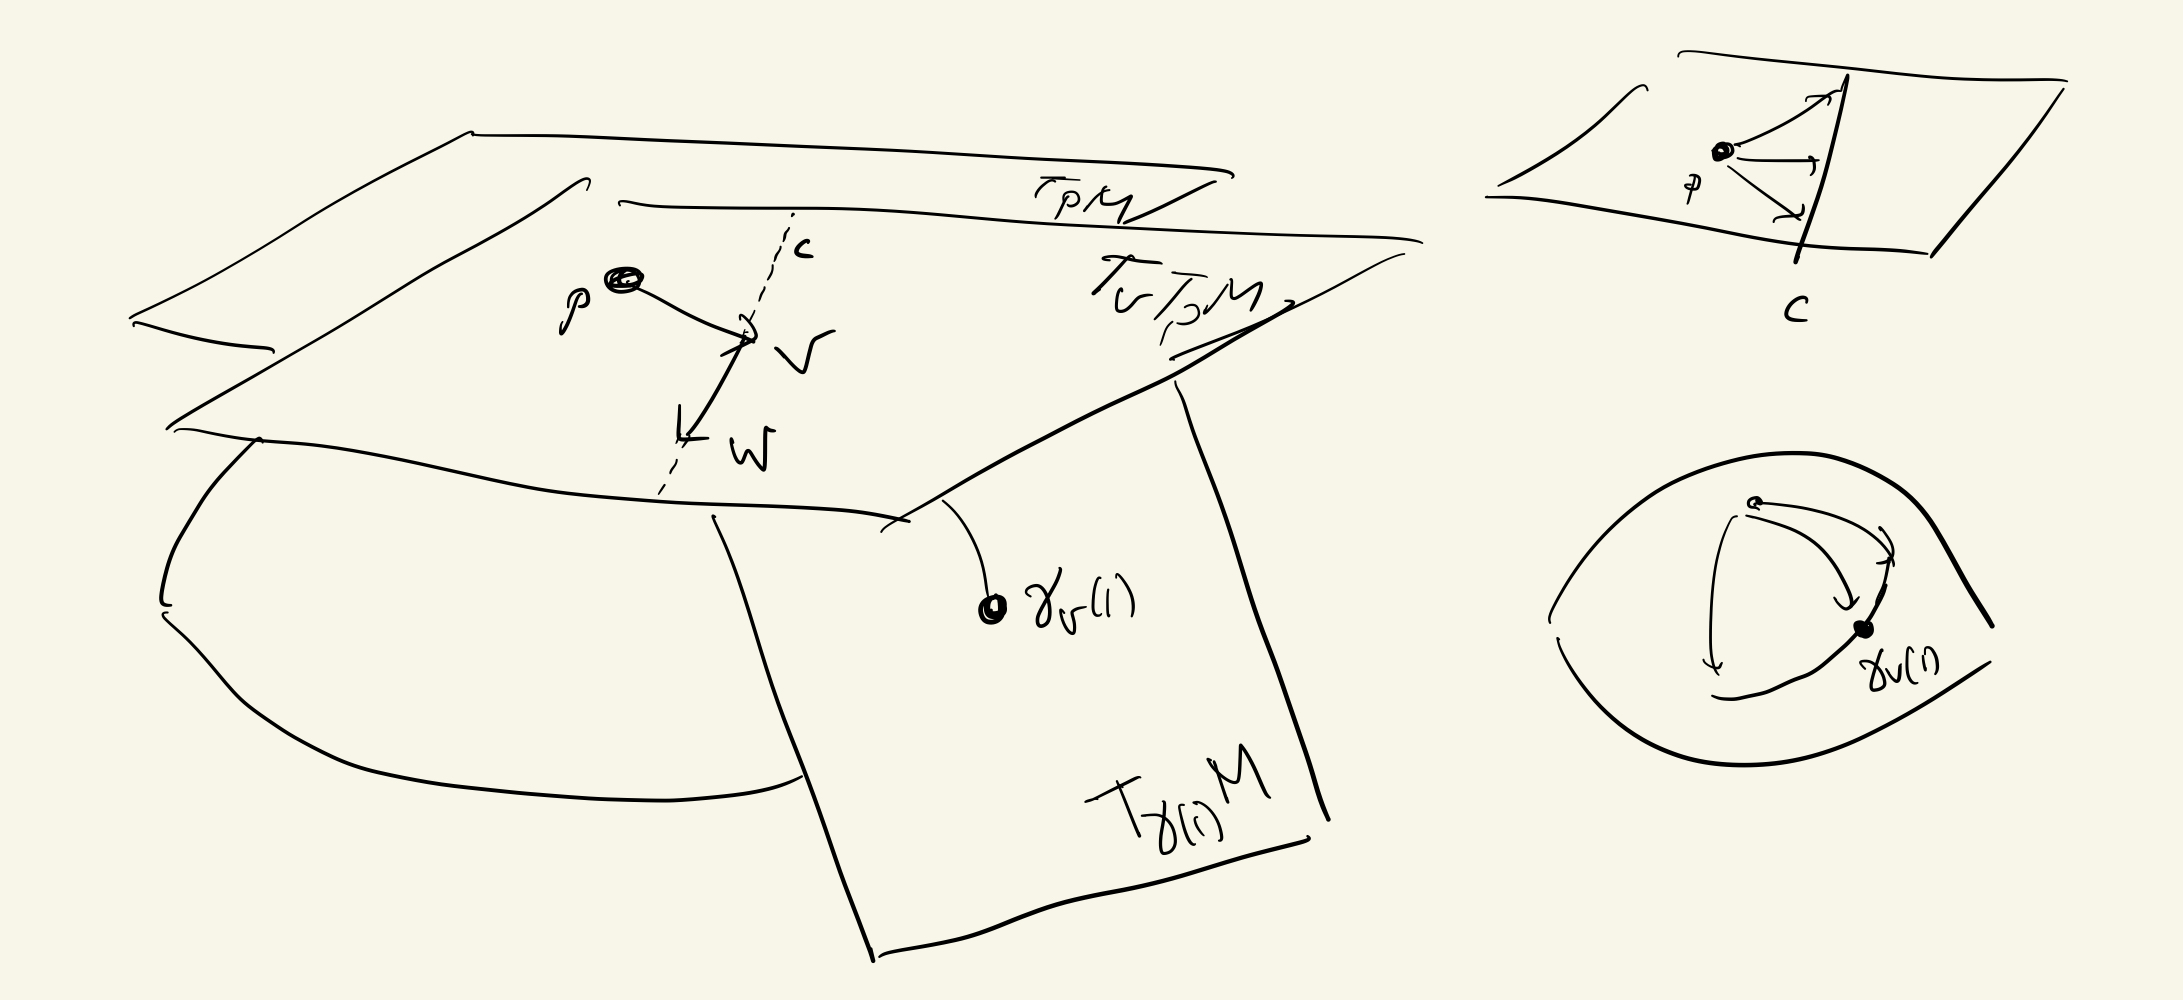
\includegraphics[width=\textwidth]{fig8}
	\end{figure}
Vamos usar o teorema de Rauch para comparar um campo de Jacobi ao longo de \(\gamma(t)=tv\) no \(T_pM\) com um campo de Jacobi ao longo da curva  \(\tilde{\gamma}(t):=\operatorname{exp}_p(tv)\). Pegue a variação no \(T_pM\) dada por \(f(t):=t(v+sw)\) onde estamos identificando \(T_vT_pM\) com \(T_pM\). É immediato que o campo variacional \(J\) é de Jacobi. De forma parecida, defina a variação \(\tilde{f}(s,t):=\operatorname{exp}_{p}(t(v+sw))\). Note que \(\tilde{f}\) é uma variação por geodésicas e portanto o campo variacional \(\tilde{J}\) é de Jacobi. Mais explicitamente, os campos de Jacobi são dados por
\[J(t)=tw,\qquad \qquad \tilde{J}(t)=d_{tv}\operatorname{exp}_{p}(tw)\]
Agora note que estamos nas condições do teorema de Rauch. Em primeiro lugar, é imediato que \(J(0)=0\) e \(\tilde{J}(0)=0\). Depois, \(|J'(0)|=|w|\) e \(|\tilde{J}'(0)|=|d_0\operatorname{exp}_p(w)|=|w|\). Por último, a condição de ortogonalidade é consequência do lema de Gauss, pois as curvas ``verticais" da variação em \(M\) percorrem esferas geodésicas.

Como a curvatura seccional de \(M\) é não negativa, concluímos que \[|tw|=|\tilde{J}|\leq |J|=|d_{tv}\operatorname{exp}_ptw|\]
para toda \(t\), incluindo \(t=1\).
\end{proof}

\begin{thing6}{Complemento}\leavevmode
Suponha adicionalmente que \(M\) é simplesmente conexa e prove que o mapa exponencial é uma expansão métrica, i.e. aumenta distâncias. Além disso, se \(M\) não é simplesmente conexa, o mapa exponencial pode não ser uma expansão métrica.
\end{thing6}

\begin{proof}[Solução]\leavevmode
	Considere um ponto arbitrário \(p \in M\), dos vetores \(v,v' \in T_pM\) e as imagens deles sob \(\operatorname{exp}_p\), digamos \(q\) e \(q'\). A distância entre \(q\) e \(q'\) é a norma do vetor velocidade de alguma geodésica minimizante \(\sigma\) tal que \(\sigma(0)=q\) e \(\sigma(1)=q'\). (Essa geodésica existe porque \(M\) é completa.)
\begin{figure}[H]
	\centering
	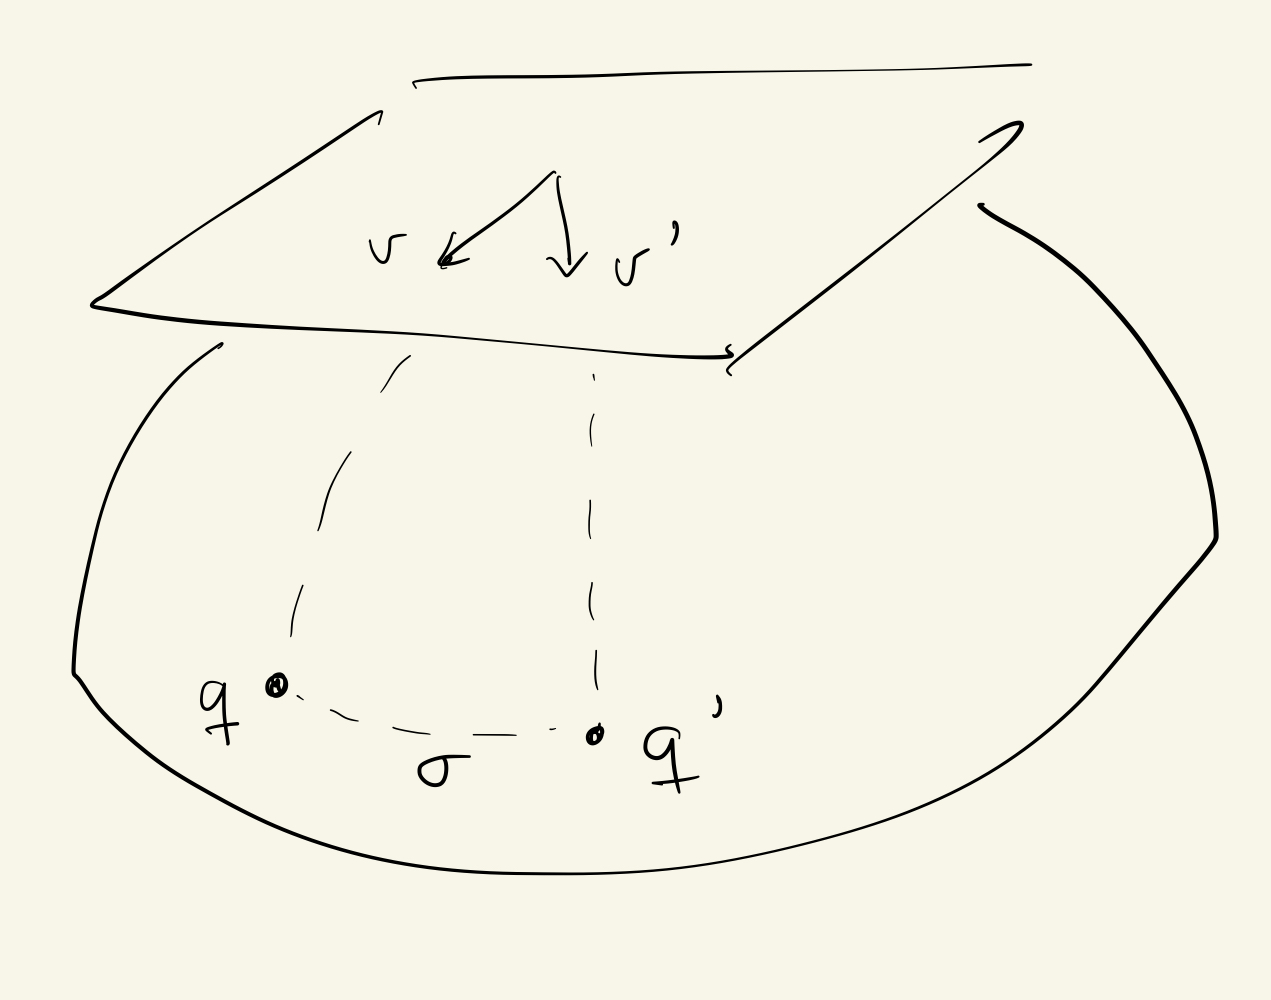
\includegraphics[width=0.5\textwidth]{fig11}
\end{figure}
Queremos comprovar que essa curva \(\sigma\) é a curva ``vertical" da variação por geodésicas do exercício anterior pegando \(w:=v'-v\). Essa curva que chamo de vertical é
\[\sigma(s):=\operatorname{exp}_p(v+sw)=\operatorname{exp}_p(v+s(v'-v))\]
(Ou seja, fixamos \(t=1\) e variamos \(s\).) Então é claro que ela chega em \(q'\) no tempo \(s=1\). Então a construção do exercício anterior aplica, e para concluir só basta mostrar que \(\sigma\) é minimizante.

Se \(\sigma\) não for minimizante, teria que existir uma outra geodésica \(\tilde{\sigma}\) ligando \(q\) e \(q'\) com comprimento menor. Como \(M\) é simplesmente conexa, essas duas curvas são homotópicas. Com um argumento análogo ao que usei no exercício 2, usando o lema de Klinenberg obtemos uma contradição usando que a curvatura de \(M\) é não positiva.


%o funcional de energia teria segunda derivada negativa em \(\sigma\) para alguma variação \(V\) de \(\sigma\). Isso diz que \(I_1(V,V)<0\) e portanto o índice de \(I_1\) não é zero, i.e. existe algum ponto conjugado pelo teorema do índice de Morse. Como mostrei no exercício 1, isso implica que \(\operatorname{exp}_p\) tem um ponto crítico, mas isso é impossível porque \(\operatorname{exp}_p\) é um difeomorfismo global já que \(M\) é simplesmente conexa (usando Hadamard).
Para um contraexemplo simples podemos usar o toro plano, que tem curvatura não positiva. É claro que a exponencial não é uma expansão métrica porque não é injetiva.
\begin{figure}[H]
	\centering
	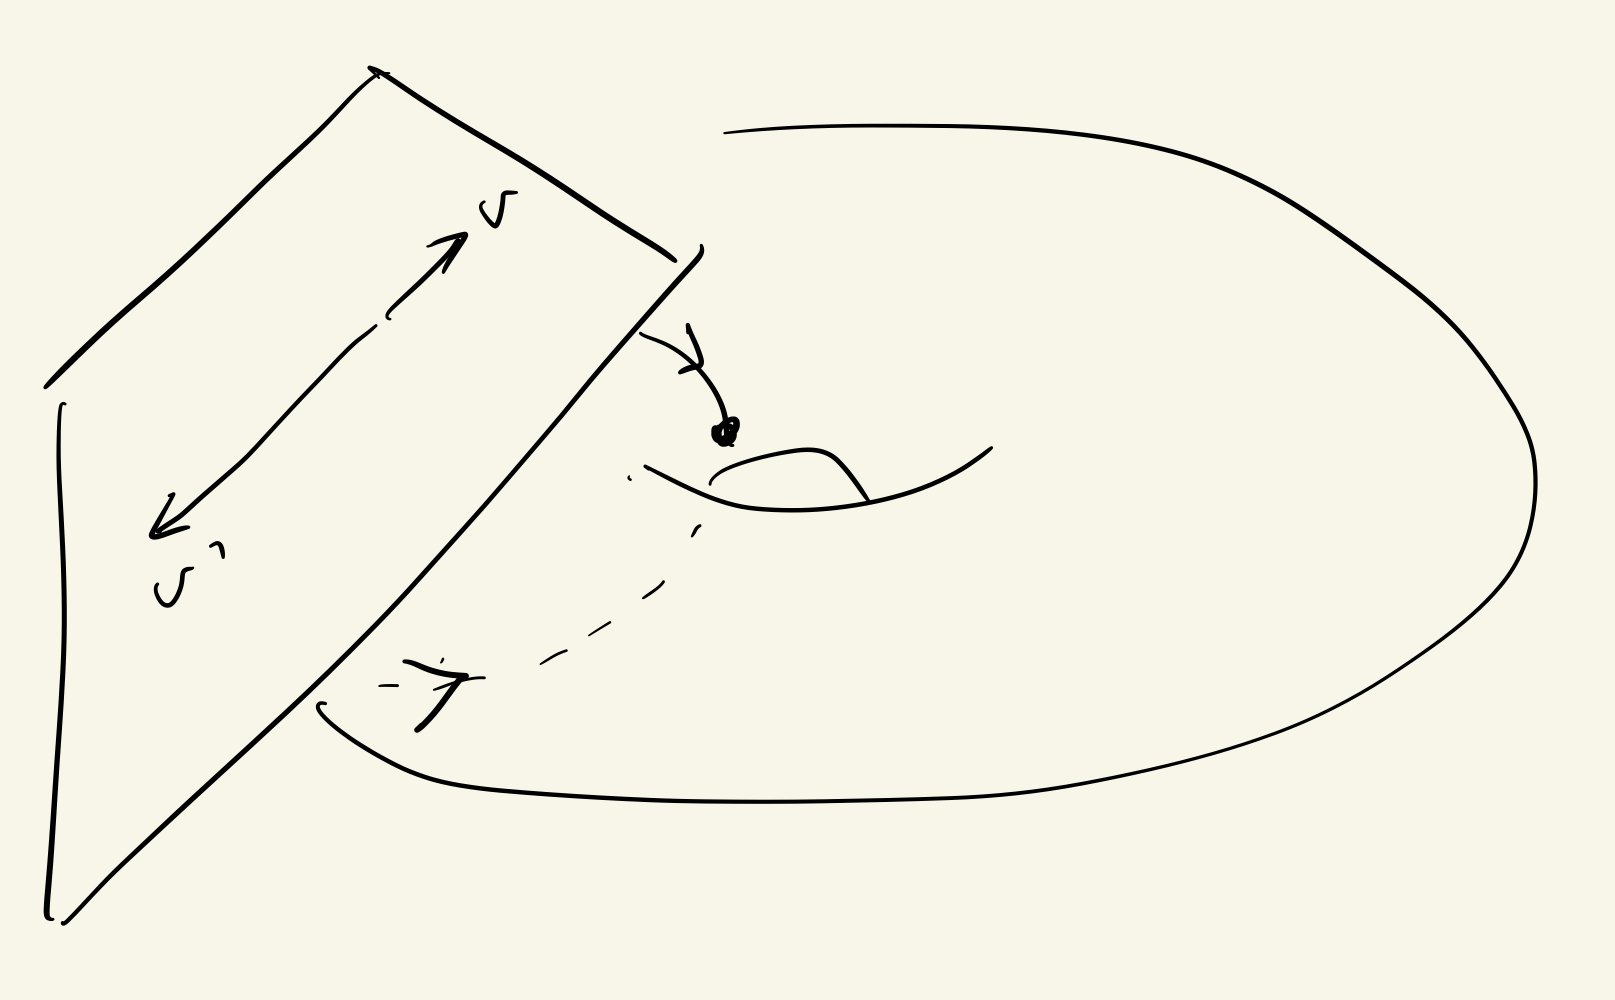
\includegraphics[width=0.6\textwidth]{fig12}
\end{figure}
\end{proof}

\begin{thing6}{Exercício 4}\label{exer:4}\leavevmode
	Seja \(\gamma:[0,a] \to M\) uma geodésica em uma variedade Riemanniana \(M\). Prove que se \(\gamma\) é minimizante, então \(\gamma\) não possui pontos conjugados em \((0,a)\). Encontre um exemplo de geodésica \(\gamma:[0,a] \to M\) sem pontos conjugados que não é minimizante.
\end{thing6}

\begin{proof}[Solução]\leavevmode
Primeiro mostro um exemplo de geodésica sem pontos conjugados que não é minimzante. Considere o cilindro \(S^1 \times \mathbb{R}\). Ele tem curvatura seccional constante igual a zero por ser um quociente de \(\mathbb{R}^2\). Isso significa que a equação de Jacobi vira \(J''+ \cancelto{0}{R_{\gamma'}J}=0\). Pegando um marco referencial paralelo \(E_i \in \mathfrak{X}_\gamma\), vemos que as funções coordenadas de \(J\) são lineares:
\[J''=(J^iE_i)''=(J^i)''E_i\]
ou seja, \(J^i=tu^i+v^i\). Agora sim, como \(J(t)=0\) então \(v^i=0\) para toda \(i\), e como \(J(t_{\operatorname{final}})=0\), também \(u^i=0\) e portanto \(J=0\). Isto é: não tem pontos conjugados em espaços de curvatura constante igual a zero.

Porém, tem geodésicas se intersectam em \(S^1\times \mathbb{R}\), que portanto não são minimizantes depois dos pontos de interseção.

\vspace{.5em}
Agora vamos mostrar que se \(\gamma\) é uma geodésica minimizante, não possui pontos conjugados em \((0,a)\). Suponha que \(b \in (0,a)\) é tal que \(\gamma(b)\) é conjugado a \(\gamma(0)\). Seguindo a prova do teorema de Jacobi dada em aula, vamos mostrar que existe uma variação própria diferenciável por partes de \(\gamma\) tal que \(E''(0)<0\) onde \(E\) denota o funcional de energia.

Considere o campo de Jacobi \(J\) tal que \(J(0)=0, J(b)=0\) que existe porque \(\gamma(b)\) é conjugado a \(\gamma(0)\). Estenda esse campo a \(\overline{J}\) como sendo 0 depois de \(b\). Considere um outro campo \(Z \in \mathfrak{X}_\gamma\). Temos que
\begin{equation}\label{eq:conju}I_a(\overline{J}+Z,\overline{J}+Z)=\cancelto{0}{I_a(\overline{J},\overline{J})}+2I_a(\overline{J},Z)+I_a(Z,Z)\end{equation}
onde a primeira parcela se anula porque \(\overline{J}\) satisfaz a equação de Jacobi antes de \(b\) e é constante zero depois de \(b\). (E usamos que \(I_a\) é simétrica, que segue das simetrias de \(R\).)

Agora vou fazer uma pausa para lembrar como se escreve a forma do índica em geral. Por definição, a forma de índice é
\[I_a(V,W):=\int_0^a \left<V'W'\right>-\int_0^a\left<R_{\gamma'}V,W\right>\]
para quaisquer campos \(V,W \in \mathfrak{X}_\gamma\).

Então reescrevemos isso usando que a conexão ao longo de \(\gamma\) é métrica:
\begin{align*}
\left<V,W'\right>'&=\left<V',W'\right>+\left<V,W''\right>\\
\implies  \left<V',W'\right>&=\left<V,W'\right>'- \left<V,W''\right>
\end{align*}
Substituindo obtemos que
\begin{align*}
I_a(V,W)&=\int_0^a\left<V,W'\right>'-\int_0^a \left<V,W''\right>-\int_0^a \left<R_{\gamma'}V,W\right>\\
&=\left<V,W'\right>|_{0}^a-\int_0^a \left<V,W''\right>-\int_0^a\left<R_{\gamma'}W,V\right>\\
&=\left<V,W'\right>|_{0}^a-\int_0^a \left<V,R_{\gamma'}W\right>
\end{align*}
Voltando ao nosso exercício, fixemos nossa atenção na parcela que está no meio em \cref{eq:conju}. Pegando \(V=Z\) e \(W=\overline{J}\) obtemos
\begin{align*}
I_a(\overline{J},Z)&=\int_0^a \cancelto{0}{\left< Z, \overline{J}'' + R_{\gamma'}\overline{J}\right>}+\int_0^a \left<Z,\overline{J}'\right>'\\&=\int_0^b\left<Z,\overline{J}'\right>'+\int_b^a \left< Z,\overline{J}'\right>'=\left<Z(b),\overline{J}'(b)\right>
\end{align*}
Agora pegue \(\delta>0\) arbitrário e considere a vizinhança de \(b\) dada por \((b-\delta,b+\delta)\). Defina \(Z\) como sendo \[Z:=\overline{J} \varphi\] onde \(\varphi\) é uma função suave que vale \(1\) em \(b\) e zero fora de \((b-\delta,b+\delta)\).

Então fica claro que \(I_a(Z,Z)\) vai ser tão pequena quanto quisermos. Note ainda que a conta que já fizemos com a quantidade  \(I_a(\overline{J},Z)\) fica inalterada com essa restrição em \(Z\); não temos problemas de diferenciabilidade e as fórmulas continuam validas.

Concluímos que
\[I_a(\overline{J}+Z,\overline{J}+Z)=-\left<\overline{J}(b)',\overline{J}(b)'\right>+\text{constante pequena} \]
Segue que \(\gamma\) não é um ponto mínimo da energia, e portanto não minimiza distância.
\end{proof}

\begin{thing6}{Exercício 6}[\cite{doc}, Exer. 1, Cap XI]\label{exer:6}\leavevmode
Prove a seguinte versão do Teorema de Bonnet-Myers: \textit{se \(M\) é completa e a curvatura seccional \(K\) satisfaz \(K \geq  \delta>0\), então \(M\) é compacta e \(\operatorname{diam}M \leq \pi/\sqrt{\delta}\)}, usando o Teorema de Comparação de Rauch e o teorema de Jacobi.
\end{thing6}

\begin{proof}[Solução]\leavevmode
	Vamos mostrar que nenhuma geodésica pode ser minimizante depois de alcançar comprimento \(\pi/\sqrt{\delta}\). Buscando uma contradição, suponha que \(\gamma\) é uma geodésica parametrizada por comprimento de arco até algum tempo maior que \(\pi/\sqrt{\delta}\). Escolha um campo de Jacobi \(J\) ao longo de \(\gamma\) ortogonal a  \(\gamma'\) e tal que \(J(0)=0\). Compare esse campo com um outro campo \(\tilde{J}\) ao longo de alguma geodésica \(\tilde{\gamma}\) em \(S^n_\delta\) satisfazendo que \(\tilde{J}(0)\), \(\tilde{J} \perp \tilde{\gamma}'\) e \(|J|=|\tilde{J}|\). (De novo, esse campo existe porque é a solução da equação de Jacobi em \(S^n_\delta\) junto com a condição de ortogonalidade.)

Como \(K \geq  \delta\) e \(\tilde{\gamma}\) não tem pontos conjugados, concluímos que \(|J|\leq |\tilde{J}|\). Mas \(\tilde{J}(\pi/\sqrt{\delta})=0\), de modo que também  \(J\) se anula quando \(\gamma\) nesse tempo. Então \(J\) é um campo de Jacobi ao longo de \(\gamma\), e pelo exercício anterior não é minimizante depois desse tempo. Como \(\gamma\) é parametrizada por comprimento de arco, segue o resultado. (O fato de \(M\) ser compacta segue de que ela tem um diâmetro finito, pois ela é um conjunto fechado e limitado.)
\end{proof}

\begin{thing7}{Observação}\leavevmode
A diferença com o teorema de Bonnet-Myers é que aquele é para \(\operatorname{Ric}\).
\end{thing7}

\begin{thing6}{Exercício 7}\label{exer:7}\leavevmode
Suponha \(M^n\) uma variedade Riemanniana com curvatura seccional \(K_M \geq 1\). Suponha que \(\gamma\) é uma geodésica em \(M\) de comprimento \(\ell(\gamma)>\pi\). Prove que \(i(\gamma)\geq n-1\), onde  \(i(\gamma)\) denota o índice de Morse de  \(\gamma\).
\end{thing6}

\begin{proof}[Solução]\leavevmode
	%Como o índice de Morse é definido como sendo o supremo das dimensões dos subespaços de \(\mathfrak{X}_\gamma\) onde \(I_\gamma\) é negativa definida, devemos mostrar que existem pelo menos \(n-1\) campos em \(\mathfrak{X}_\gamma\) linearmente independentes tais que \(I_a\) seja negativa definida no espaço vetorial gerado por esses campos.
Lembre o seguinte fato geral mostrado em aula:
	\begin{equation}\label{eq:segue}\dim\{J \in \mathfrak{X}^J_\gamma:J(0)=0, J \perp \gamma\}=n-1\end{equation}
Isso segue das seguintes observações:
\begin{enumerate}[label=(\alph*)]
\item \(\dim\mathfrak{X}^J_\gamma=2n\) porque são soluções de \(n\) equações diferenciais ordinárias de segunda ordem, i.e. cada campo de Jacobi está determinado pelas condições iniciais \(J(0)\) e \(J'(0)\). 
\item \(\dim \{J \in \mathfrak{X}^J_\gamma:J(0)=0\}=n\).
\item \(\dim \{J \in \mathfrak{X}^J_\gamma:J\perp \gamma'\}=2n-2\). Para confirmar isso note que pelas simetrias de \(R\) e a equação de Jacobi tem-se que \(\left<J,\gamma'\right>''=0\), pelo que \(\left<J,\gamma'\right>=a+bt\) para dois números reais \(a,b\). Segue que qualquer \(J \in \mathfrak{X}^J_\gamma\) se escreve como \(J(t)=a\gamma'(t)+bt\gamma'(t)+\hat{J}(t)\) para algum \(\hat{J}\) perpendicular a  \(\gamma'\). (Supondo que \(|\gamma'|=1\).) Então se \(J \perp \gamma\), temos que  \(a=b=0\), então tiramos dois números do \(2n\) que tínhamos.
\item Segue \cref{eq:segue}.
\end{enumerate}
Lembre também que o teorema do índice de Morse (cf. \cite{doc}) diz que o índice \(i(\gamma)\) é igual ao numero de pontos \(\gamma(t)\), \(0<t<a\) conjugados a \(\gamma(0)\) ao longo de \(\gamma\) contando a multiplicidade (a multiplicidade de um ponto conjugado é a dimensão do espaço de campos de Jacobi que se anulam nos extremos).

Portanto para nosso exercício basta achar \(n-1\) pontos conjugados a \(\gamma(0)\). Isso fica resolvido tomando \(n-1\) campos de Jacobi ortogonais a \(\gamma'\), que sabemos que existem pelo comentário anterior. Aplicando para cada um deles o teorema de comparação de Rauch como no exercício anterior comprovamos que eles se anulam quando \(\gamma\) atinge comprimento \(\pi\), obtendo assim os \(n-1\) pontos conjugados que buscávamos.

Note que \(\gamma\) pode ter ainda mais pontos conjugados depois de \(\gamma(\pi)\), de modo que o índice \(i(\gamma)\) pode ser ainda maior.
\end{proof}

\begin{thing7}{Dúvida}\leavevmode
Estudando a prova do teorema do índice de Morse, usamos que kernel da forma do índice \(I_\gamma\) consiste exatamente dos campos de Jacobi (usando conta que fiz no exercício 4, e graças à simetria de  \(I_\gamma\)). Então \textit{parece} que não estamos buscando \(n-1\) campos de campos de Jacobi linearmente independes: estamos buscando \(n-1\) campos linearmente independentes tais que \(I_a\) restrita ao espaço gerado por esses campos seja negativa definida.
\end{thing7}

\bibliography{bib.bib}


\end{document}
